% Options for packages loaded elsewhere
\PassOptionsToPackage{unicode}{hyperref}
\PassOptionsToPackage{hyphens}{url}
%
\documentclass[
]{book}
\usepackage{amsmath,amssymb}
\usepackage{lmodern}
\usepackage{iftex}
\ifPDFTeX
  \usepackage[T1]{fontenc}
  \usepackage[utf8]{inputenc}
  \usepackage{textcomp} % provide euro and other symbols
\else % if luatex or xetex
  \usepackage{unicode-math}
  \defaultfontfeatures{Scale=MatchLowercase}
  \defaultfontfeatures[\rmfamily]{Ligatures=TeX,Scale=1}
\fi
% Use upquote if available, for straight quotes in verbatim environments
\IfFileExists{upquote.sty}{\usepackage{upquote}}{}
\IfFileExists{microtype.sty}{% use microtype if available
  \usepackage[]{microtype}
  \UseMicrotypeSet[protrusion]{basicmath} % disable protrusion for tt fonts
}{}
\makeatletter
\@ifundefined{KOMAClassName}{% if non-KOMA class
  \IfFileExists{parskip.sty}{%
    \usepackage{parskip}
  }{% else
    \setlength{\parindent}{0pt}
    \setlength{\parskip}{6pt plus 2pt minus 1pt}}
}{% if KOMA class
  \KOMAoptions{parskip=half}}
\makeatother
\usepackage{xcolor}
\usepackage{color}
\usepackage{fancyvrb}
\newcommand{\VerbBar}{|}
\newcommand{\VERB}{\Verb[commandchars=\\\{\}]}
\DefineVerbatimEnvironment{Highlighting}{Verbatim}{commandchars=\\\{\}}
% Add ',fontsize=\small' for more characters per line
\usepackage{framed}
\definecolor{shadecolor}{RGB}{248,248,248}
\newenvironment{Shaded}{\begin{snugshade}}{\end{snugshade}}
\newcommand{\AlertTok}[1]{\textcolor[rgb]{0.94,0.16,0.16}{#1}}
\newcommand{\AnnotationTok}[1]{\textcolor[rgb]{0.56,0.35,0.01}{\textbf{\textit{#1}}}}
\newcommand{\AttributeTok}[1]{\textcolor[rgb]{0.77,0.63,0.00}{#1}}
\newcommand{\BaseNTok}[1]{\textcolor[rgb]{0.00,0.00,0.81}{#1}}
\newcommand{\BuiltInTok}[1]{#1}
\newcommand{\CharTok}[1]{\textcolor[rgb]{0.31,0.60,0.02}{#1}}
\newcommand{\CommentTok}[1]{\textcolor[rgb]{0.56,0.35,0.01}{\textit{#1}}}
\newcommand{\CommentVarTok}[1]{\textcolor[rgb]{0.56,0.35,0.01}{\textbf{\textit{#1}}}}
\newcommand{\ConstantTok}[1]{\textcolor[rgb]{0.00,0.00,0.00}{#1}}
\newcommand{\ControlFlowTok}[1]{\textcolor[rgb]{0.13,0.29,0.53}{\textbf{#1}}}
\newcommand{\DataTypeTok}[1]{\textcolor[rgb]{0.13,0.29,0.53}{#1}}
\newcommand{\DecValTok}[1]{\textcolor[rgb]{0.00,0.00,0.81}{#1}}
\newcommand{\DocumentationTok}[1]{\textcolor[rgb]{0.56,0.35,0.01}{\textbf{\textit{#1}}}}
\newcommand{\ErrorTok}[1]{\textcolor[rgb]{0.64,0.00,0.00}{\textbf{#1}}}
\newcommand{\ExtensionTok}[1]{#1}
\newcommand{\FloatTok}[1]{\textcolor[rgb]{0.00,0.00,0.81}{#1}}
\newcommand{\FunctionTok}[1]{\textcolor[rgb]{0.00,0.00,0.00}{#1}}
\newcommand{\ImportTok}[1]{#1}
\newcommand{\InformationTok}[1]{\textcolor[rgb]{0.56,0.35,0.01}{\textbf{\textit{#1}}}}
\newcommand{\KeywordTok}[1]{\textcolor[rgb]{0.13,0.29,0.53}{\textbf{#1}}}
\newcommand{\NormalTok}[1]{#1}
\newcommand{\OperatorTok}[1]{\textcolor[rgb]{0.81,0.36,0.00}{\textbf{#1}}}
\newcommand{\OtherTok}[1]{\textcolor[rgb]{0.56,0.35,0.01}{#1}}
\newcommand{\PreprocessorTok}[1]{\textcolor[rgb]{0.56,0.35,0.01}{\textit{#1}}}
\newcommand{\RegionMarkerTok}[1]{#1}
\newcommand{\SpecialCharTok}[1]{\textcolor[rgb]{0.00,0.00,0.00}{#1}}
\newcommand{\SpecialStringTok}[1]{\textcolor[rgb]{0.31,0.60,0.02}{#1}}
\newcommand{\StringTok}[1]{\textcolor[rgb]{0.31,0.60,0.02}{#1}}
\newcommand{\VariableTok}[1]{\textcolor[rgb]{0.00,0.00,0.00}{#1}}
\newcommand{\VerbatimStringTok}[1]{\textcolor[rgb]{0.31,0.60,0.02}{#1}}
\newcommand{\WarningTok}[1]{\textcolor[rgb]{0.56,0.35,0.01}{\textbf{\textit{#1}}}}
\usepackage{longtable,booktabs,array}
\usepackage{calc} % for calculating minipage widths
% Correct order of tables after \paragraph or \subparagraph
\usepackage{etoolbox}
\makeatletter
\patchcmd\longtable{\par}{\if@noskipsec\mbox{}\fi\par}{}{}
\makeatother
% Allow footnotes in longtable head/foot
\IfFileExists{footnotehyper.sty}{\usepackage{footnotehyper}}{\usepackage{footnote}}
\makesavenoteenv{longtable}
\usepackage{graphicx}
\makeatletter
\def\maxwidth{\ifdim\Gin@nat@width>\linewidth\linewidth\else\Gin@nat@width\fi}
\def\maxheight{\ifdim\Gin@nat@height>\textheight\textheight\else\Gin@nat@height\fi}
\makeatother
% Scale images if necessary, so that they will not overflow the page
% margins by default, and it is still possible to overwrite the defaults
% using explicit options in \includegraphics[width, height, ...]{}
\setkeys{Gin}{width=\maxwidth,height=\maxheight,keepaspectratio}
% Set default figure placement to htbp
\makeatletter
\def\fps@figure{htbp}
\makeatother
\setlength{\emergencystretch}{3em} % prevent overfull lines
\providecommand{\tightlist}{%
  \setlength{\itemsep}{0pt}\setlength{\parskip}{0pt}}
\setcounter{secnumdepth}{5}
\ifLuaTeX
  \usepackage{selnolig}  % disable illegal ligatures
\fi
\usepackage[]{natbib}
\bibliographystyle{apalike}
\nocite{*}
\IfFileExists{bookmark.sty}{\usepackage{bookmark}}{\usepackage{hyperref}}
\IfFileExists{xurl.sty}{\usepackage{xurl}}{} % add URL line breaks if available
\urlstyle{same} % disable monospaced font for URLs
\hypersetup{
  pdftitle={Supplemental Material for Phylogeny-informed fitness estimation},
  pdfauthor={Alexander Lalejini, Matthew Andres Moreno, Jose Guadalupe Hernandez, and Emily Dolson},
  hidelinks,
  pdfcreator={LaTeX via pandoc}}

\title{Supplemental Material for Phylogeny-informed fitness estimation}
\author{Alexander Lalejini, Matthew Andres Moreno, Jose Guadalupe Hernandez, and Emily Dolson}
\date{2023-05-15}

\begin{document}
\maketitle

{
\setcounter{tocdepth}{1}
\tableofcontents
}
\hypertarget{introduction}{%
\chapter{Introduction}\label{introduction}}

This is the supplemental material for our submission to Genetic Programming Theory and Practice XX.
This is not intended as a stand-alone document, but as a companion to our manuscript.

\hypertarget{about-our-supplemental-material}{%
\section{About our supplemental material}\label{about-our-supplemental-material}}

As you may have noticed (unless you're reading a pdf version of this), our supplemental material is hosted using \href{https://pages.github.com/}{GitHub pages}.
We compiled our data analyses and supplemental documentation into this nifty web-accessible book using \href{https://bookdown.org}{bookdown}.

The source code/configuration files for this supplemental material can be found in \href{https://github.com/amlalejini/phylogeny-informed-evaluation}{this GitHub repository}.

Our supplemental material includes the following:

\begin{itemize}
\tightlist
\item
  Data availability (Section \ref{data-availability})
\item
  GP instruction set (Section \ref{signalgp-instruction-set})
\item
  Analysis notebooks for each experiment (including source code)

  \begin{itemize}
  \tightlist
  \item
    Selection scheme diagnostics (Section \ref{selection-scheme-diagnostic-experiments})
  \item
    Program synthesis problems (Section TODO)
  \end{itemize}
\end{itemize}

\hypertarget{contributing-authors}{%
\section{Contributing authors}\label{contributing-authors}}

\begin{itemize}
\tightlist
\item
  Alexander Lalejini
\item
  Matthew Andres Moreno
\item
  Jose Guadalupe Hernandez
\item
  Emily Dolson
\end{itemize}

\hypertarget{data-availability}{%
\chapter{Data Availability}\label{data-availability}}

\hypertarget{source-code}{%
\section{Source code}\label{source-code}}

The source code for this work is publicly accessible on GitHub: \url{https://github.com/amlalejini/phylogeny-informed-evaluation}.

\hypertarget{experiment-software-dependencies}{%
\subsection{Experiment software dependencies}\label{experiment-software-dependencies}}

\begin{itemize}
\tightlist
\item
  SignalGP: \url{https://github.com/amlalejini/SignalGP}

  \begin{itemize}
  \tightlist
  \item
    commit hash: \texttt{8cc56a79aa6b2655bacefcc7b63ee6a859c730f3}
  \end{itemize}
\item
  Empirical: \url{https://github.com/devosoft/Empirical}

  \begin{itemize}
  \tightlist
  \item
    commit hash: \texttt{5955a1cae2a5de36aa3a65df060a56b38f575bd0}
  \end{itemize}
\end{itemize}

\hypertarget{training-and-testing-sets}{%
\section{Training and testing sets}\label{training-and-testing-sets}}

The training and testing sets used for program synthesis problems can be found on GitHub: \url{https://github.com/amlalejini/phylogeny-informed-evaluation/tree/main/experiments/2023-05-08-psynth/hpc/config}.

\hypertarget{experimental-results}{%
\section{Experimental results}\label{experimental-results}}

All of our experimental data is available online from our OSF respository: \url{https://osf.io/wxckn/}

\hypertarget{signalgp-instruction-set}{%
\chapter{SignalGP instruction set}\label{signalgp-instruction-set}}

Below, we document the instruction set used in our GP system for our 2023 GPTP experiments.

Abbreviations:

\begin{itemize}
\tightlist
\item
  EOP: End of program
\item
  Reg: local register

  \begin{itemize}
  \tightlist
  \item
    Reg{[}0{]} indicates the value at the register specified by an instruction's first \emph{argument}, Reg{[}1{]} indicates the value at the register specified by an instruction's second argument, and Reg{[}2{]} indicates the value at the register specified by the instruction's third argument.
  \item
    Reg{[}0{]}, Reg{[}1{]}, \emph{etc}: Register 0, Register 1, \emph{etc.}
  \end{itemize}
\item
  Input: input buffer

  \begin{itemize}
  \tightlist
  \item
    Follows same scheme as Reg
  \end{itemize}
\item
  Output: output buffer

  \begin{itemize}
  \tightlist
  \item
    Follows same scheme as Reg
  \end{itemize}
\item
  Global: global memory buffer

  \begin{itemize}
  \tightlist
  \item
    Follows same scheme as Reg
  \end{itemize}
\item
  Arg: Instruction argument

  \begin{itemize}
  \tightlist
  \item
    Arg{[}i{]} indicates the i'th instruction argument (an integer encoded in the genome)
  \item
    E.g., Arg{[}0{]} is an instruction's first argument
  \end{itemize}
\end{itemize}

Instructions that would produce undefined behavior (e.g., division by zero) are treated as no operations.

\hypertarget{default-instructions}{%
\section{Default Instructions}\label{default-instructions}}

I.e., instructions used across all diagnostic tasks.

\begin{longtable}[]{@{}
  >{\raggedright\arraybackslash}p{(\columnwidth - 4\tabcolsep) * \real{0.3077}}
  >{\centering\arraybackslash}p{(\columnwidth - 4\tabcolsep) * \real{0.3846}}
  >{\raggedright\arraybackslash}p{(\columnwidth - 4\tabcolsep) * \real{0.3077}}@{}}
\toprule()
\begin{minipage}[b]{\linewidth}\raggedright
Instruction
\end{minipage} & \begin{minipage}[b]{\linewidth}\centering
Arguments Used
\end{minipage} & \begin{minipage}[b]{\linewidth}\raggedright
Description
\end{minipage} \\
\midrule()
\endhead
\texttt{Nop} & 0 & No operation \\
\texttt{Not} & 1 & Reg{[}0{]} = !Reg{[}0{]} \\
\texttt{Inc} & 1 & Reg{[}0{]} = Reg{[}0{]} + 1 \\
\texttt{Dec} & 1 & Reg{[}0{]} = Reg{[}0{]} - 1 \\
\texttt{Add} & 3 & Reg{[}2{]} = Reg{[}0{]} + Reg{[}1{]} \\
\texttt{Sub} & 3 & Reg{[}2{]} = Reg{[}0{]} - Reg{[}1{]} \\
\texttt{Mult} & 3 & Reg{[}2{]} = Reg{[}0{]} * Reg{[}1{]} \\
\texttt{Div} & 3 & Reg{[}2{]} = Reg{[}0{]} / Reg{[}1{]} \\
\texttt{Mod} & 3 & Reg{[}2{]} = Reg{[}0{]} \% Reg{[}1{]} \\
\texttt{Nand} & 2 & Reg{[}2{]} = !(Reg{[}0{]} \& Reg{[}1{]}) \\
\texttt{TestEqu} & 3 & Reg{[}2{]} = Reg{[}0{]} == Reg{[}1{]} \\
\texttt{TestNEqu} & 3 & Reg{[}2{]} = Reg{[}0{]} != Reg{[}1{]} \\
\texttt{TestLess} & 3 & Reg{[}2{]} = Reg{[}0{]} \textless{} Reg{[}1{]} \\
\texttt{TestLessEqu} & 3 & Reg{[}2{]} = Reg{[}0{]} \textless= Reg{[}1{]} \\
\texttt{TestGreater} & 3 & Reg{[}2{]} = Reg{[}0{]} \textgreater{} Reg{[}1{]} \\
\texttt{TestGreaterEqu} & 3 & Reg{[}2{]} = Reg{[}0{]} \textgreater= Reg{[}1{]} \\
\texttt{SetMem} & 2 & Reg{[}0{]} = Arg{[}1{]} \\
\texttt{Terminal} & 1 & Reg{[}0{]} = double value encoded by instruction tag \\
\texttt{CopyMem} & 2 & Reg{[}0{]} = Reg{[}1{]} \\
\texttt{SwapMem} & 2 & Swap(Reg{[}0{]}, Reg{[}1{]}) \\
\texttt{InputToWorking} & 2 & Reg{[}1{]} = Input{[}0{]} \\
\texttt{WorkingToOutput} & 2 & Output{[}1{]} = Reg{[}0{]} \\
\texttt{If} & 1 & If Reg{[}0{]} != 0, proceed. Otherwise skip to the next \texttt{Close} or EOP. \\
\texttt{While} & 1 & While Reg{[}0{]} != 0, loop. Otherwise skip to next \texttt{Close} or EOP. \\
\texttt{Close} & 0 & Indicate the end of a control block of code (e.g., loop, if). \\
\texttt{Break} & 0 & Break out of current control flow (e.g., loop). \\
\texttt{Call} & 0 & Call a function, using this instruction's tag to determine which function is called. \\
\texttt{Routine} & 0 & Same as call, but local memory is shared. Sort of like a jump that will jump back when the routine ends. \\
\texttt{Return} & 0 & Return from the current function call. \\
\texttt{WorkingToGlobal} & 2 & Global{[}1{]} = Reg{[}0{]} \\
\texttt{GlobalToWorking} & 2 & Reg{[}1{]} = Global{[}0{]} \\
\texttt{FullGlobalToWorking} & 0 & Copy entire global memory buffer into working memory buffer \\
\texttt{FullWorkingToGlobal} & 0 & Copy entire working memory buffer into global memory buffer \\
\bottomrule()
\end{longtable}

Note that \texttt{Nand} performs a bitwise operation.

\hypertarget{problem-specific-instructions}{%
\section{Problem-specific instructions}\label{problem-specific-instructions}}

Each problem has problem-specific instructions for producing output.

\hypertarget{fizz-buzz}{%
\subsection{Fizz Buzz}\label{fizz-buzz}}

\begin{itemize}
\tightlist
\item
  SubmitFizz
\item
  SubmitBuzz
\item
  SubmitFizzBuzz
\item
  SubmitEcho
\end{itemize}

\hypertarget{median}{%
\subsection{Median}\label{median}}

\begin{itemize}
\tightlist
\item
  SubmitOutput
\end{itemize}

\hypertarget{grade}{%
\subsection{Grade}\label{grade}}

\begin{itemize}
\tightlist
\item
  SubmitA
\item
  SubmitB
\item
  SubmitC
\item
  SubmitD
\item
  SubmitF
\end{itemize}

\hypertarget{small-or-large}{%
\subsection{Small or large}\label{small-or-large}}

\begin{itemize}
\tightlist
\item
  SubmitSmall
\item
  SubmitLarge
\item
  SubmitNeither
\end{itemize}

\hypertarget{selection-scheme-diagnostic-experiments}{%
\chapter{Selection scheme diagnostic experiments}\label{selection-scheme-diagnostic-experiments}}

\begin{Shaded}
\begin{Highlighting}[]
\NormalTok{experiment\_slug }\OtherTok{\textless{}{-}} \StringTok{"2023{-}05{-}10{-}diagnostics"}

\NormalTok{working\_directory }\OtherTok{\textless{}{-}} \FunctionTok{paste0}\NormalTok{(}
  \StringTok{"experiments/"}\NormalTok{,}
\NormalTok{  experiment\_slug,}
  \StringTok{"/analysis/"}
\NormalTok{)}

\ControlFlowTok{if}\NormalTok{ (}\FunctionTok{exists}\NormalTok{(}\StringTok{"bookdown\_wd\_prefix"}\NormalTok{)) \{}
\NormalTok{  working\_directory }\OtherTok{\textless{}{-}} \FunctionTok{paste0}\NormalTok{(}
\NormalTok{    bookdown\_wd\_prefix,}
\NormalTok{    working\_directory}
\NormalTok{  )}
\NormalTok{\}}
\end{Highlighting}
\end{Shaded}

\hypertarget{dependencies}{%
\section{Dependencies}\label{dependencies}}

\begin{Shaded}
\begin{Highlighting}[]
\FunctionTok{library}\NormalTok{(tidyverse)}
\end{Highlighting}
\end{Shaded}

\begin{verbatim}
## -- Attaching packages ----------------------------------------------------------------------------------------------------------------------------------------------------------------- tidyverse 1.3.2 --
## v ggplot2 3.3.6     v purrr   1.0.1
## v tibble  3.1.8     v dplyr   1.1.0
## v tidyr   1.3.0     v stringr 1.5.0
## v readr   2.1.3     v forcats 0.5.2
## -- Conflicts -------------------------------------------------------------------------------------------------------------------------------------------------------------------- tidyverse_conflicts() --
## x dplyr::filter() masks stats::filter()
## x dplyr::lag()    masks stats::lag()
\end{verbatim}

\begin{Shaded}
\begin{Highlighting}[]
\FunctionTok{library}\NormalTok{(ggplot2)}
\FunctionTok{library}\NormalTok{(cowplot)}
\FunctionTok{library}\NormalTok{(RColorBrewer)}
\FunctionTok{library}\NormalTok{(khroma)}
\FunctionTok{library}\NormalTok{(rstatix)}
\end{Highlighting}
\end{Shaded}

\begin{verbatim}
## 
## Attaching package: 'rstatix'
## 
## The following object is masked from 'package:stats':
## 
##     filter
\end{verbatim}

\begin{Shaded}
\begin{Highlighting}[]
\FunctionTok{library}\NormalTok{(knitr)}
\FunctionTok{source}\NormalTok{(}\StringTok{"https://gist.githubusercontent.com/benmarwick/2a1bb0133ff568cbe28d/raw/fb53bd97121f7f9ce947837ef1a4c65a73bffb3f/geom\_flat\_violin.R"}\NormalTok{)}
\end{Highlighting}
\end{Shaded}

\begin{Shaded}
\begin{Highlighting}[]
\FunctionTok{print}\NormalTok{(version)}
\end{Highlighting}
\end{Shaded}

\begin{verbatim}
##                _                           
## platform       aarch64-apple-darwin20      
## arch           aarch64                     
## os             darwin20                    
## system         aarch64, darwin20           
## status                                     
## major          4                           
## minor          2.1                         
## year           2022                        
## month          06                          
## day            23                          
## svn rev        82513                       
## language       R                           
## version.string R version 4.2.1 (2022-06-23)
## nickname       Funny-Looking Kid
\end{verbatim}

\hypertarget{setup}{%
\section{Setup}\label{setup}}

\begin{Shaded}
\begin{Highlighting}[]
\CommentTok{\# Configure our default graphing theme}
\FunctionTok{theme\_set}\NormalTok{(}\FunctionTok{theme\_cowplot}\NormalTok{())}
\CommentTok{\# Create a directory to store plots}
\NormalTok{plot\_directory }\OtherTok{\textless{}{-}} \FunctionTok{paste0}\NormalTok{(working\_directory, }\StringTok{"plots/"}\NormalTok{)}
\FunctionTok{dir.create}\NormalTok{(plot\_directory, }\AttributeTok{showWarnings=}\ConstantTok{FALSE}\NormalTok{)}
\end{Highlighting}
\end{Shaded}

\hypertarget{load-experiment-summary-data}{%
\subsection{Load experiment summary data}\label{load-experiment-summary-data}}

\begin{Shaded}
\begin{Highlighting}[]
\NormalTok{summary\_data\_loc }\OtherTok{\textless{}{-}} \FunctionTok{paste0}\NormalTok{(working\_directory, }\StringTok{"data/aggregate.csv"}\NormalTok{)}
\NormalTok{summary\_data }\OtherTok{\textless{}{-}} \FunctionTok{read\_csv}\NormalTok{(summary\_data\_loc)}
\end{Highlighting}
\end{Shaded}

\begin{verbatim}
## Rows: 520 Columns: 49
## -- Column specification ----------------------------------------------------------------------------------------------------------------------------------------------------------------------------------
## Delimiter: ","
## chr  (5): DIAGNOSTIC, EVAL_FIT_EST_MODE, EVAL_MODE, SELECTION, STOP_MODE
## dbl (44): ACCURACY, CREDIT, DIAGNOSTIC_DIMENSIONALITY, GENE_LOWER_BND, GENE_...
## 
## i Use `spec()` to retrieve the full column specification for this data.
## i Specify the column types or set `show_col_types = FALSE` to quiet this message.
\end{verbatim}

\begin{Shaded}
\begin{Highlighting}[]
\NormalTok{summary\_data }\OtherTok{\textless{}{-}}\NormalTok{ summary\_data }\SpecialCharTok{\%\textgreater{}\%}
  \FunctionTok{mutate}\NormalTok{(}
    \AttributeTok{eval\_mode\_row =} \FunctionTok{case\_when}\NormalTok{(}
\NormalTok{      EVAL\_MODE }\SpecialCharTok{==} \StringTok{"full"} \SpecialCharTok{\&}\NormalTok{ TEST\_DOWNSAMPLE\_RATE }\SpecialCharTok{==} \StringTok{"1"} \SpecialCharTok{\textasciitilde{}} \StringTok{"down{-}sample"}\NormalTok{,}
\NormalTok{      EVAL\_MODE }\SpecialCharTok{==} \StringTok{"full"} \SpecialCharTok{\&}\NormalTok{ NUM\_COHORTS }\SpecialCharTok{==} \StringTok{"1"} \SpecialCharTok{\textasciitilde{}} \StringTok{"cohort"}\NormalTok{,}
      \AttributeTok{.default =}\NormalTok{ EVAL\_MODE}
\NormalTok{    ),}
    \AttributeTok{evals\_per\_gen =} \FunctionTok{case\_when}\NormalTok{(}
\NormalTok{      EVAL\_MODE }\SpecialCharTok{==} \StringTok{"cohort{-}full{-}compete"} \SpecialCharTok{\textasciitilde{}} \FloatTok{1.0} \SpecialCharTok{/}\NormalTok{ NUM\_COHORTS,}
\NormalTok{      EVAL\_MODE }\SpecialCharTok{==} \StringTok{"cohort"} \SpecialCharTok{\textasciitilde{}} \FloatTok{1.0} \SpecialCharTok{/}\NormalTok{ NUM\_COHORTS,}
\NormalTok{      EVAL\_MODE }\SpecialCharTok{==} \StringTok{"down{-}sample"} \SpecialCharTok{\textasciitilde{}}\NormalTok{ TEST\_DOWNSAMPLE\_RATE,}
\NormalTok{      EVAL\_MODE }\SpecialCharTok{==} \StringTok{"full"} \SpecialCharTok{\textasciitilde{}} \FloatTok{1.0}
\NormalTok{    ),}
    \AttributeTok{EVAL\_FIT\_EST\_MODE =} \FunctionTok{case\_when}\NormalTok{(}
\NormalTok{      EVAL\_FIT\_EST\_MODE }\SpecialCharTok{==} \StringTok{"ancestor{-}opt"} \SpecialCharTok{\textasciitilde{}} \StringTok{"ancestor"}\NormalTok{,}
\NormalTok{      EVAL\_FIT\_EST\_MODE }\SpecialCharTok{==} \StringTok{"relative{-}opt"} \SpecialCharTok{\textasciitilde{}} \StringTok{"relative"}\NormalTok{,}
      \AttributeTok{.default =}\NormalTok{ EVAL\_FIT\_EST\_MODE}
\NormalTok{    ),}
    \AttributeTok{.keep =} \StringTok{"all"}
\NormalTok{  ) }\SpecialCharTok{\%\textgreater{}\%}
  \FunctionTok{mutate}\NormalTok{(}
    \AttributeTok{evals\_per\_gen =} \FunctionTok{as.factor}\NormalTok{(evals\_per\_gen),}
    \AttributeTok{eval\_mode\_row =} \FunctionTok{as.factor}\NormalTok{(eval\_mode\_row),}
    \AttributeTok{DIAGNOSTIC =} \FunctionTok{as.factor}\NormalTok{(DIAGNOSTIC),}
    \AttributeTok{SELECTION =} \FunctionTok{as.factor}\NormalTok{(SELECTION),}
    \AttributeTok{EVAL\_MODE =} \FunctionTok{as.factor}\NormalTok{(EVAL\_MODE),}
    \AttributeTok{NUM\_COHORTS =} \FunctionTok{as.factor}\NormalTok{(NUM\_COHORTS),}
    \AttributeTok{TEST\_DOWNSAMPLE\_RATE =} \FunctionTok{as.factor}\NormalTok{(TEST\_DOWNSAMPLE\_RATE),}
    \AttributeTok{EVAL\_FIT\_EST\_MODE =} \FunctionTok{factor}\NormalTok{(}
\NormalTok{      EVAL\_FIT\_EST\_MODE,}
      \AttributeTok{levels =} \FunctionTok{c}\NormalTok{(}
        \StringTok{"none"}\NormalTok{,}
        \StringTok{"ancestor"}\NormalTok{,}
        \StringTok{"relative"}
\NormalTok{      ),}
      \AttributeTok{labels =} \FunctionTok{c}\NormalTok{(}
        \StringTok{"None"}\NormalTok{,}
        \StringTok{"Ancestor"}\NormalTok{,}
        \StringTok{"Relative"}
\NormalTok{      )}
\NormalTok{    )}
\NormalTok{  )}

\CommentTok{\# Split summary data on diagnostic}
\NormalTok{con\_obj\_summary\_data }\OtherTok{\textless{}{-}} \FunctionTok{filter}\NormalTok{(}
\NormalTok{  summary\_data,}
\NormalTok{  DIAGNOSTIC }\SpecialCharTok{==} \StringTok{"contradictory{-}objectives"}
\NormalTok{)}

\NormalTok{explore\_summary\_data }\OtherTok{\textless{}{-}} \FunctionTok{filter}\NormalTok{(}
\NormalTok{  summary\_data,}
\NormalTok{  DIAGNOSTIC }\SpecialCharTok{==} \StringTok{"multipath{-}exploration"}
\NormalTok{)}
\end{Highlighting}
\end{Shaded}

\hypertarget{load-experiment-time-series-data}{%
\subsection{Load experiment time series data}\label{load-experiment-time-series-data}}

\begin{Shaded}
\begin{Highlighting}[]
\NormalTok{ts\_data\_loc }\OtherTok{\textless{}{-}} \FunctionTok{paste0}\NormalTok{(working\_directory, }\StringTok{"data/time\_series.csv"}\NormalTok{)}
\NormalTok{ts\_data }\OtherTok{\textless{}{-}} \FunctionTok{read\_csv}\NormalTok{(ts\_data\_loc)}
\end{Highlighting}
\end{Shaded}

\begin{verbatim}
## Rows: 104000 Columns: 19
## -- Column specification ----------------------------------------------------------------------------------------------------------------------------------------------------------------------------------
## Delimiter: ","
## chr  (4): DIAGNOSTIC, EVAL_FIT_EST_MODE, EVAL_MODE, SELECTION
## dbl (15): NUM_COHORTS, SEED, TEST_DOWNSAMPLE_RATE, entropy_selected_ids, eva...
## 
## i Use `spec()` to retrieve the full column specification for this data.
## i Specify the column types or set `show_col_types = FALSE` to quiet this message.
\end{verbatim}

\begin{Shaded}
\begin{Highlighting}[]
\NormalTok{ts\_data }\OtherTok{\textless{}{-}}\NormalTok{ ts\_data }\SpecialCharTok{\%\textgreater{}\%}
  \FunctionTok{mutate}\NormalTok{(}
    \AttributeTok{eval\_mode\_row =} \FunctionTok{case\_when}\NormalTok{(}
\NormalTok{      EVAL\_MODE }\SpecialCharTok{==} \StringTok{"full"} \SpecialCharTok{\&}\NormalTok{ TEST\_DOWNSAMPLE\_RATE }\SpecialCharTok{==} \StringTok{"1"} \SpecialCharTok{\textasciitilde{}} \StringTok{"down{-}sample"}\NormalTok{,}
\NormalTok{      EVAL\_MODE }\SpecialCharTok{==} \StringTok{"full"} \SpecialCharTok{\&}\NormalTok{ NUM\_COHORTS }\SpecialCharTok{==} \StringTok{"1"} \SpecialCharTok{\textasciitilde{}} \StringTok{"cohort"}\NormalTok{,}
      \AttributeTok{.default =}\NormalTok{ EVAL\_MODE}
\NormalTok{    ),}
    \AttributeTok{evals\_per\_gen =} \FunctionTok{case\_when}\NormalTok{(}
\NormalTok{      EVAL\_MODE }\SpecialCharTok{==} \StringTok{"cohort{-}full{-}compete"} \SpecialCharTok{\textasciitilde{}} \FloatTok{1.0} \SpecialCharTok{/}\NormalTok{ NUM\_COHORTS,}
\NormalTok{      EVAL\_MODE }\SpecialCharTok{==} \StringTok{"cohort"} \SpecialCharTok{\textasciitilde{}} \FloatTok{1.0} \SpecialCharTok{/}\NormalTok{ NUM\_COHORTS,}
\NormalTok{      EVAL\_MODE }\SpecialCharTok{==} \StringTok{"down{-}sample"} \SpecialCharTok{\textasciitilde{}}\NormalTok{ TEST\_DOWNSAMPLE\_RATE,}
\NormalTok{      EVAL\_MODE }\SpecialCharTok{==} \StringTok{"full"} \SpecialCharTok{\textasciitilde{}} \FloatTok{1.0}
\NormalTok{    ),}
    \AttributeTok{EVAL\_FIT\_EST\_MODE =} \FunctionTok{case\_when}\NormalTok{(}
\NormalTok{      EVAL\_FIT\_EST\_MODE }\SpecialCharTok{==} \StringTok{"ancestor{-}opt"} \SpecialCharTok{\textasciitilde{}} \StringTok{"ancestor"}\NormalTok{,}
\NormalTok{      EVAL\_FIT\_EST\_MODE }\SpecialCharTok{==} \StringTok{"relative{-}opt"} \SpecialCharTok{\textasciitilde{}} \StringTok{"relative"}\NormalTok{,}
      \AttributeTok{.default =}\NormalTok{ EVAL\_FIT\_EST\_MODE}
\NormalTok{    ),}
    \AttributeTok{.keep =} \StringTok{"all"}
\NormalTok{  ) }\SpecialCharTok{\%\textgreater{}\%}
  \FunctionTok{mutate}\NormalTok{(}
    \AttributeTok{evals\_per\_gen =} \FunctionTok{as.factor}\NormalTok{(evals\_per\_gen),}
    \AttributeTok{DIAGNOSTIC =} \FunctionTok{as.factor}\NormalTok{(DIAGNOSTIC),}
    \AttributeTok{SELECTION =} \FunctionTok{as.factor}\NormalTok{(SELECTION),}
    \AttributeTok{EVAL\_MODE =} \FunctionTok{as.factor}\NormalTok{(EVAL\_MODE),}
    \AttributeTok{NUM\_COHORTS =} \FunctionTok{as.factor}\NormalTok{(NUM\_COHORTS),}
    \AttributeTok{TEST\_DOWNSAMPLE\_RATE =} \FunctionTok{as.factor}\NormalTok{(TEST\_DOWNSAMPLE\_RATE),}
    \AttributeTok{EVAL\_FIT\_EST\_MODE =} \FunctionTok{factor}\NormalTok{(}
\NormalTok{      EVAL\_FIT\_EST\_MODE,}
      \AttributeTok{levels =} \FunctionTok{c}\NormalTok{(}
        \StringTok{"none"}\NormalTok{,}
        \StringTok{"ancestor"}\NormalTok{,}
        \StringTok{"relative"}
\NormalTok{      ),}
      \AttributeTok{labels =} \FunctionTok{c}\NormalTok{(}
        \StringTok{"None"}\NormalTok{,}
        \StringTok{"Ancestor"}\NormalTok{,}
        \StringTok{"Relative"}
\NormalTok{      )}
\NormalTok{    )}
\NormalTok{  )}

\NormalTok{con\_obj\_ts\_data }\OtherTok{\textless{}{-}}\NormalTok{ ts\_data }\SpecialCharTok{\%\textgreater{}\%}
  \FunctionTok{filter}\NormalTok{(DIAGNOSTIC }\SpecialCharTok{==} \StringTok{"contradictory{-}objectives"}\NormalTok{)}

\NormalTok{explore\_ts\_data }\OtherTok{\textless{}{-}}\NormalTok{ ts\_data }\SpecialCharTok{\%\textgreater{}\%}
  \FunctionTok{filter}\NormalTok{(DIAGNOSTIC }\SpecialCharTok{==} \StringTok{"multipath{-}exploration"}\NormalTok{)}
\end{Highlighting}
\end{Shaded}

\hypertarget{load-estimate-source-distributions}{%
\subsection{Load estimate source distributions}\label{load-estimate-source-distributions}}

\begin{Shaded}
\begin{Highlighting}[]
\NormalTok{est\_source\_data }\OtherTok{\textless{}{-}} \FunctionTok{read\_csv}\NormalTok{(}
  \FunctionTok{paste0}\NormalTok{(working\_directory, }\StringTok{"data/phylo{-}est{-}info.csv"}\NormalTok{)}
\NormalTok{)}
\end{Highlighting}
\end{Shaded}

\begin{verbatim}
## Rows: 520 Columns: 38
## -- Column specification ----------------------------------------------------------------------------------------------------------------------------------------------------------------------------------
## Delimiter: ","
## chr  (6): OUTPUT_DIR, DIAGNOSTIC, STOP_MODE, SELECTION, EVAL_MODE, EVAL_FIT_...
## dbl (32): SNAPSHOT_INTERVAL, OUTPUT_SUMMARY_DATA_INTERVAL, MUTATE_STD, TARGE...
## 
## i Use `spec()` to retrieve the full column specification for this data.
## i Specify the column types or set `show_col_types = FALSE` to quiet this message.
\end{verbatim}

\begin{Shaded}
\begin{Highlighting}[]
\NormalTok{est\_source\_data }\OtherTok{\textless{}{-}}\NormalTok{ est\_source\_data }\SpecialCharTok{\%\textgreater{}\%}
  \FunctionTok{mutate}\NormalTok{(}
    \AttributeTok{eval\_mode\_row =} \FunctionTok{case\_when}\NormalTok{(}
\NormalTok{      EVAL\_MODE }\SpecialCharTok{==} \StringTok{"full"} \SpecialCharTok{\&}\NormalTok{ TEST\_DOWNSAMPLE\_RATE }\SpecialCharTok{==} \StringTok{"1"} \SpecialCharTok{\textasciitilde{}} \StringTok{"down{-}sample"}\NormalTok{,}
\NormalTok{      EVAL\_MODE }\SpecialCharTok{==} \StringTok{"full"} \SpecialCharTok{\&}\NormalTok{ NUM\_COHORTS }\SpecialCharTok{==} \StringTok{"1"} \SpecialCharTok{\textasciitilde{}} \StringTok{"cohort"}\NormalTok{,}
      \AttributeTok{.default =}\NormalTok{ EVAL\_MODE}
\NormalTok{    ),}
    \AttributeTok{evals\_per\_gen =} \FunctionTok{case\_when}\NormalTok{(}
\NormalTok{      EVAL\_MODE }\SpecialCharTok{==} \StringTok{"cohort{-}full{-}compete"} \SpecialCharTok{\textasciitilde{}} \FloatTok{1.0} \SpecialCharTok{/}\NormalTok{ NUM\_COHORTS,}
\NormalTok{      EVAL\_MODE }\SpecialCharTok{==} \StringTok{"cohort"} \SpecialCharTok{\textasciitilde{}} \FloatTok{1.0} \SpecialCharTok{/}\NormalTok{ NUM\_COHORTS,}
\NormalTok{      EVAL\_MODE }\SpecialCharTok{==} \StringTok{"down{-}sample"} \SpecialCharTok{\textasciitilde{}}\NormalTok{ TEST\_DOWNSAMPLE\_RATE,}
\NormalTok{      EVAL\_MODE }\SpecialCharTok{==} \StringTok{"full"} \SpecialCharTok{\textasciitilde{}} \FloatTok{1.0}
\NormalTok{    ),}
    \AttributeTok{EVAL\_FIT\_EST\_MODE =} \FunctionTok{case\_when}\NormalTok{(}
\NormalTok{      EVAL\_FIT\_EST\_MODE }\SpecialCharTok{==} \StringTok{"ancestor{-}opt"} \SpecialCharTok{\textasciitilde{}} \StringTok{"ancestor"}\NormalTok{,}
\NormalTok{      EVAL\_FIT\_EST\_MODE }\SpecialCharTok{==} \StringTok{"relative{-}opt"} \SpecialCharTok{\textasciitilde{}} \StringTok{"relative"}\NormalTok{,}
      \AttributeTok{.default =}\NormalTok{ EVAL\_FIT\_EST\_MODE}
\NormalTok{    ),}
    \AttributeTok{.keep =} \StringTok{"all"}
\NormalTok{  ) }\SpecialCharTok{\%\textgreater{}\%}
  \FunctionTok{mutate}\NormalTok{(}
    \AttributeTok{evals\_per\_gen =} \FunctionTok{as.factor}\NormalTok{(evals\_per\_gen),}
    \AttributeTok{eval\_mode\_row =} \FunctionTok{as.factor}\NormalTok{(eval\_mode\_row),}
    \AttributeTok{DIAGNOSTIC =} \FunctionTok{as.factor}\NormalTok{(DIAGNOSTIC),}
    \AttributeTok{SELECTION =} \FunctionTok{as.factor}\NormalTok{(SELECTION),}
    \AttributeTok{EVAL\_MODE =} \FunctionTok{as.factor}\NormalTok{(EVAL\_MODE),}
    \AttributeTok{NUM\_COHORTS =} \FunctionTok{as.factor}\NormalTok{(NUM\_COHORTS),}
    \AttributeTok{TEST\_DOWNSAMPLE\_RATE =} \FunctionTok{as.factor}\NormalTok{(TEST\_DOWNSAMPLE\_RATE),}
    \AttributeTok{EVAL\_FIT\_EST\_MODE =} \FunctionTok{factor}\NormalTok{(}
\NormalTok{      EVAL\_FIT\_EST\_MODE,}
      \AttributeTok{levels =} \FunctionTok{c}\NormalTok{(}
        \StringTok{"none"}\NormalTok{,}
        \StringTok{"ancestor"}\NormalTok{,}
        \StringTok{"relative"}
\NormalTok{      ),}
      \AttributeTok{labels =} \FunctionTok{c}\NormalTok{(}
        \StringTok{"None"}\NormalTok{,}
        \StringTok{"Ancestor"}\NormalTok{,}
        \StringTok{"Relative"}
\NormalTok{      )}
\NormalTok{    )}
\NormalTok{  ) }\SpecialCharTok{\%\textgreater{}\%}
  \FunctionTok{mutate}\NormalTok{(}
    \AttributeTok{prop\_self\_lookups =} \FunctionTok{case\_when}\NormalTok{(}
\NormalTok{      (EVAL\_MODE }\SpecialCharTok{!=} \StringTok{"full"} \SpecialCharTok{\&}\NormalTok{ EVAL\_FIT\_EST\_MODE }\SpecialCharTok{!=} \StringTok{"None"}\NormalTok{) }\SpecialCharTok{\textasciitilde{}}
\NormalTok{        self\_count }\SpecialCharTok{/}\NormalTok{ (other\_count }\SpecialCharTok{+}\NormalTok{ ancestor\_count }\SpecialCharTok{+}\NormalTok{ descendant\_count }\SpecialCharTok{+}\NormalTok{ self\_count }\SpecialCharTok{+}\NormalTok{ outside\_count),}
      \AttributeTok{.default =} \DecValTok{0}
\NormalTok{    ),}
    \AttributeTok{prop\_other\_lookups =}  \FunctionTok{case\_when}\NormalTok{(}
\NormalTok{      (EVAL\_MODE }\SpecialCharTok{!=} \StringTok{"full"} \SpecialCharTok{\&}\NormalTok{ EVAL\_FIT\_EST\_MODE }\SpecialCharTok{!=} \StringTok{"None"}\NormalTok{) }\SpecialCharTok{\textasciitilde{}}
\NormalTok{        other\_count }\SpecialCharTok{/}\NormalTok{ (other\_count }\SpecialCharTok{+}\NormalTok{ ancestor\_count }\SpecialCharTok{+}\NormalTok{ descendant\_count }\SpecialCharTok{+}\NormalTok{ self\_count }\SpecialCharTok{+}\NormalTok{ outside\_count),}
      \AttributeTok{.default =} \DecValTok{0}
\NormalTok{    ),}
    \AttributeTok{prop\_ancestor\_lookups =}  \FunctionTok{case\_when}\NormalTok{(}
\NormalTok{      (EVAL\_MODE }\SpecialCharTok{!=} \StringTok{"full"} \SpecialCharTok{\&}\NormalTok{ EVAL\_FIT\_EST\_MODE }\SpecialCharTok{!=} \StringTok{"None"}\NormalTok{) }\SpecialCharTok{\textasciitilde{}}
\NormalTok{        ancestor\_count }\SpecialCharTok{/}\NormalTok{ (other\_count }\SpecialCharTok{+}\NormalTok{ ancestor\_count }\SpecialCharTok{+}\NormalTok{ descendant\_count }\SpecialCharTok{+}\NormalTok{ self\_count }\SpecialCharTok{+}\NormalTok{ outside\_count),}
      \AttributeTok{.default =} \DecValTok{0}
\NormalTok{    ),}
    \AttributeTok{prop\_descendant\_lookups =} \FunctionTok{case\_when}\NormalTok{(}
\NormalTok{      (EVAL\_MODE }\SpecialCharTok{!=} \StringTok{"full"} \SpecialCharTok{\&}\NormalTok{ EVAL\_FIT\_EST\_MODE }\SpecialCharTok{!=} \StringTok{"None"}\NormalTok{) }\SpecialCharTok{\textasciitilde{}}
\NormalTok{        descendant\_count }\SpecialCharTok{/}\NormalTok{ (other\_count }\SpecialCharTok{+}\NormalTok{ ancestor\_count }\SpecialCharTok{+}\NormalTok{ descendant\_count }\SpecialCharTok{+}\NormalTok{ self\_count }\SpecialCharTok{+}\NormalTok{ outside\_count),}
      \AttributeTok{.default =} \DecValTok{0}
\NormalTok{    ),}
    \AttributeTok{prop\_outside\_lookups =}  \FunctionTok{case\_when}\NormalTok{(}
\NormalTok{      (EVAL\_MODE }\SpecialCharTok{!=} \StringTok{"full"} \SpecialCharTok{\&}\NormalTok{ EVAL\_FIT\_EST\_MODE }\SpecialCharTok{!=} \StringTok{"None"}\NormalTok{) }\SpecialCharTok{\textasciitilde{}}
\NormalTok{        outside\_count }\SpecialCharTok{/}\NormalTok{ (other\_count }\SpecialCharTok{+}\NormalTok{ ancestor\_count }\SpecialCharTok{+}\NormalTok{ descendant\_count }\SpecialCharTok{+}\NormalTok{ self\_count }\SpecialCharTok{+}\NormalTok{ outside\_count),}
      \AttributeTok{.default =} \DecValTok{0}
\NormalTok{    )}
\NormalTok{  )}
\end{Highlighting}
\end{Shaded}

\hypertarget{contradictory-objectives-diagnostic}{%
\section{Contradictory objectives diagnostic}\label{contradictory-objectives-diagnostic}}

\hypertarget{population-wide-satisfactory-trait-coverage-final}{%
\subsection{Population-wide satisfactory trait coverage (final)}\label{population-wide-satisfactory-trait-coverage-final}}

Satifactory trait coverage after 50,000 generations:

\begin{Shaded}
\begin{Highlighting}[]
\NormalTok{contradictory\_obj\_final\_plt }\OtherTok{\textless{}{-}} \FunctionTok{ggplot}\NormalTok{(}
\NormalTok{    con\_obj\_summary\_data,}
    \FunctionTok{aes}\NormalTok{(}
      \AttributeTok{x =}\NormalTok{ EVAL\_FIT\_EST\_MODE,}
      \AttributeTok{y =}\NormalTok{ pop\_optimal\_trait\_coverage,}
      \AttributeTok{fill =}\NormalTok{ EVAL\_FIT\_EST\_MODE}
\NormalTok{    )}
\NormalTok{  ) }\SpecialCharTok{+}
  \FunctionTok{geom\_flat\_violin}\NormalTok{(}
    \AttributeTok{position =} \FunctionTok{position\_nudge}\NormalTok{(}\AttributeTok{x =}\NormalTok{ .}\DecValTok{2}\NormalTok{, }\AttributeTok{y =} \DecValTok{0}\NormalTok{),}
    \AttributeTok{alpha =}\NormalTok{ .}\DecValTok{8}\NormalTok{,}
    \AttributeTok{adjust=}\FloatTok{1.5}
\NormalTok{  ) }\SpecialCharTok{+}
  \FunctionTok{geom\_point}\NormalTok{(}
    \AttributeTok{mapping=}\FunctionTok{aes}\NormalTok{(}\AttributeTok{color=}\NormalTok{EVAL\_FIT\_EST\_MODE),}
    \AttributeTok{position =} \FunctionTok{position\_jitter}\NormalTok{(}\AttributeTok{width =}\NormalTok{ .}\DecValTok{15}\NormalTok{),}
    \AttributeTok{size =}\NormalTok{ .}\DecValTok{5}\NormalTok{,}
    \AttributeTok{alpha =} \FloatTok{0.8}
\NormalTok{  ) }\SpecialCharTok{+}
  \FunctionTok{geom\_boxplot}\NormalTok{(}
    \AttributeTok{width =}\NormalTok{ .}\DecValTok{1}\NormalTok{,}
    \AttributeTok{outlier.shape =} \ConstantTok{NA}\NormalTok{,}
    \AttributeTok{alpha =} \FloatTok{0.5}
\NormalTok{  ) }\SpecialCharTok{+}
  \FunctionTok{scale\_y\_continuous}\NormalTok{(}
    \CommentTok{\# limits = c({-}0.5, 100)}
\NormalTok{  ) }\SpecialCharTok{+}
  \FunctionTok{scale\_fill\_bright}\NormalTok{() }\SpecialCharTok{+}
  \FunctionTok{scale\_color\_bright}\NormalTok{() }\SpecialCharTok{+}
  \FunctionTok{facet\_grid}\NormalTok{(}
\NormalTok{    eval\_mode\_row}\SpecialCharTok{\textasciitilde{}}\NormalTok{evals\_per\_gen,}
    \CommentTok{\# nrow=2,}
    \AttributeTok{labeller=}\NormalTok{label\_both}
\NormalTok{  ) }\SpecialCharTok{+}
  \FunctionTok{theme}\NormalTok{(}
    \AttributeTok{legend.position =} \StringTok{"none"}\NormalTok{,}
    \AttributeTok{axis.text.x =} \FunctionTok{element\_text}\NormalTok{(}
      \AttributeTok{angle =} \DecValTok{30}\NormalTok{,}
      \AttributeTok{hjust =} \DecValTok{1}
\NormalTok{    ),}
    \AttributeTok{panel.border =} \FunctionTok{element\_rect}\NormalTok{(}\AttributeTok{color=}\StringTok{"gray"}\NormalTok{, }\AttributeTok{size=}\DecValTok{2}\NormalTok{)}
\NormalTok{  )}
\FunctionTok{ggsave}\NormalTok{(}
  \AttributeTok{filename =} \FunctionTok{paste0}\NormalTok{(plot\_directory, }\StringTok{"contra{-}obj{-}final.pdf"}\NormalTok{),}
  \AttributeTok{plot =}\NormalTok{ contradictory\_obj\_final\_plt }\SpecialCharTok{+} \FunctionTok{labs}\NormalTok{(}\AttributeTok{title=}\StringTok{"Contradictory objectives"}\NormalTok{),}
  \AttributeTok{width =} \DecValTok{15}\NormalTok{,}
  \AttributeTok{height =} \DecValTok{10}
\NormalTok{)}
\end{Highlighting}
\end{Shaded}

\begin{Shaded}
\begin{Highlighting}[]
\NormalTok{contradictory\_obj\_final\_plt}
\end{Highlighting}
\end{Shaded}

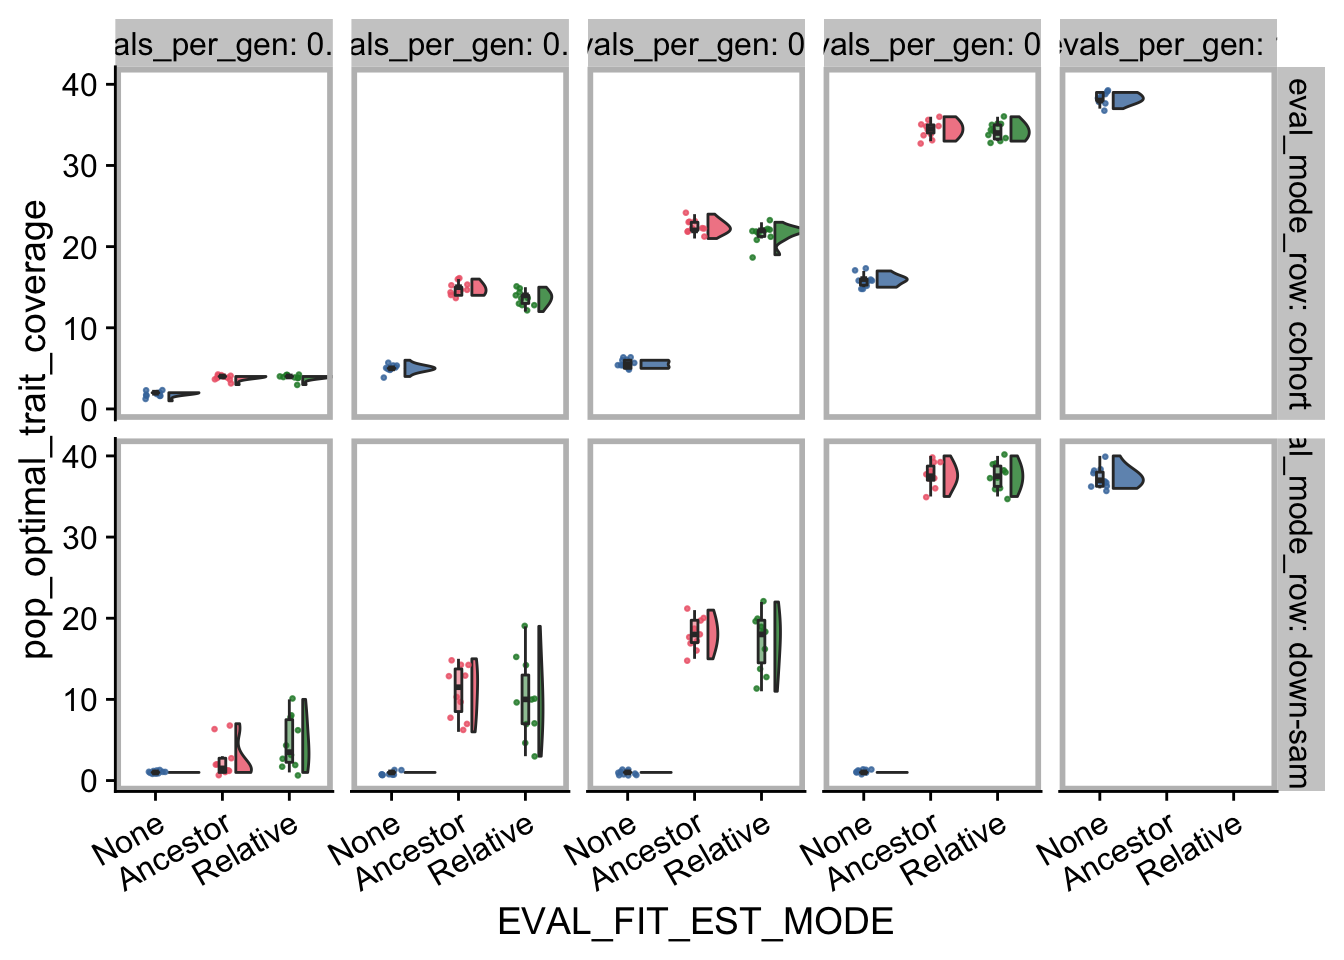
\includegraphics{phylogeny-informed-estimation-supplemental_files/figure-latex/unnamed-chunk-10-1.pdf}

\hypertarget{statistical-analysis}{%
\subsubsection{Statistical analysis}\label{statistical-analysis}}

First, we create a table of summary values for satisfactory trait coverage in the final generation.

\begin{Shaded}
\begin{Highlighting}[]
\NormalTok{con\_obj\_summary\_data }\SpecialCharTok{\%\textgreater{}\%}
  \FunctionTok{filter}\NormalTok{(EVAL\_MODE }\SpecialCharTok{!=} \StringTok{"full"}\NormalTok{) }\SpecialCharTok{\%\textgreater{}\%}
  \FunctionTok{group\_by}\NormalTok{(EVAL\_MODE, evals\_per\_gen, EVAL\_FIT\_EST\_MODE) }\SpecialCharTok{\%\textgreater{}\%}
  \FunctionTok{summarize}\NormalTok{(}
    \AttributeTok{cov\_median =} \FunctionTok{median}\NormalTok{(pop\_optimal\_trait\_coverage),}
    \AttributeTok{cov\_mean =} \FunctionTok{mean}\NormalTok{(pop\_optimal\_trait\_coverage),}
    \AttributeTok{n =} \FunctionTok{n}\NormalTok{()}
\NormalTok{  ) }\SpecialCharTok{\%\textgreater{}\%}
  \FunctionTok{kable}\NormalTok{()}
\end{Highlighting}
\end{Shaded}

\begin{verbatim}
## `summarise()` has grouped output by 'EVAL_MODE', 'evals_per_gen'. You can
## override using the `.groups` argument.
\end{verbatim}

\begin{tabular}{l|l|l|r|r|r}
\hline
EVAL\_MODE & evals\_per\_gen & EVAL\_FIT\_EST\_MODE & cov\_median & cov\_mean & n\\
\hline
cohort & 0.01 & None & 2.0 & 1.9 & 10\\
\hline
cohort & 0.01 & Ancestor & 4.0 & 3.9 & 10\\
\hline
cohort & 0.01 & Relative & 4.0 & 3.9 & 10\\
\hline
cohort & 0.05 & None & 5.0 & 5.0 & 10\\
\hline
cohort & 0.05 & Ancestor & 15.0 & 14.8 & 10\\
\hline
cohort & 0.05 & Relative & 14.0 & 13.7 & 10\\
\hline
cohort & 0.1 & None & 5.5 & 5.5 & 10\\
\hline
cohort & 0.1 & Ancestor & 22.0 & 22.4 & 10\\
\hline
cohort & 0.1 & Relative & 22.0 & 21.6 & 10\\
\hline
cohort & 0.5 & None & 16.0 & 15.9 & 10\\
\hline
cohort & 0.5 & Ancestor & 34.5 & 34.5 & 10\\
\hline
cohort & 0.5 & Relative & 34.0 & 34.2 & 10\\
\hline
down-sample & 0.01 & None & 1.0 & 1.0 & 10\\
\hline
down-sample & 0.01 & Ancestor & 1.5 & 2.5 & 10\\
\hline
down-sample & 0.01 & Relative & 3.5 & 4.7 & 10\\
\hline
down-sample & 0.05 & None & 1.0 & 1.0 & 10\\
\hline
down-sample & 0.05 & Ancestor & 11.5 & 11.0 & 10\\
\hline
down-sample & 0.05 & Relative & 10.0 & 10.0 & 10\\
\hline
down-sample & 0.1 & None & 1.0 & 1.0 & 10\\
\hline
down-sample & 0.1 & Ancestor & 18.0 & 18.1 & 10\\
\hline
down-sample & 0.1 & Relative & 18.0 & 17.1 & 10\\
\hline
down-sample & 0.5 & None & 1.0 & 1.0 & 10\\
\hline
down-sample & 0.5 & Ancestor & 37.5 & 37.6 & 10\\
\hline
down-sample & 0.5 & Relative & 37.5 & 37.5 & 10\\
\hline
\end{tabular}

Next, we perform a Kruskal-Wallis test to determine which comparisons contain statistically significant differences among treatments.

\begin{Shaded}
\begin{Highlighting}[]
\NormalTok{con\_obj\_kw\_test }\OtherTok{\textless{}{-}}\NormalTok{ con\_obj\_summary\_data }\SpecialCharTok{\%\textgreater{}\%}
  \FunctionTok{filter}\NormalTok{(EVAL\_MODE }\SpecialCharTok{!=} \StringTok{"full"}\NormalTok{) }\SpecialCharTok{\%\textgreater{}\%}
  \FunctionTok{group\_by}\NormalTok{(EVAL\_MODE, evals\_per\_gen) }\SpecialCharTok{\%\textgreater{}\%}
  \FunctionTok{kruskal\_test}\NormalTok{(pop\_optimal\_trait\_coverage }\SpecialCharTok{\textasciitilde{}}\NormalTok{ EVAL\_FIT\_EST\_MODE) }\SpecialCharTok{\%\textgreater{}\%}
  \FunctionTok{unite}\NormalTok{(}
    \StringTok{"comparison\_group"}\NormalTok{,}
\NormalTok{    EVAL\_MODE,}
\NormalTok{    evals\_per\_gen,}
    \AttributeTok{sep =} \StringTok{"\_"}\NormalTok{,}
    \AttributeTok{remove =} \ConstantTok{FALSE}
\NormalTok{  )}

\FunctionTok{kable}\NormalTok{(con\_obj\_kw\_test)}
\end{Highlighting}
\end{Shaded}

\begin{tabular}{l|l|l|l|r|r|r|r|l}
\hline
comparison\_group & EVAL\_MODE & evals\_per\_gen & .y. & n & statistic & df & p & method\\
\hline
cohort\_0.01 & cohort & 0.01 & pop\_optimal\_trait\_coverage & 30 & 25.55066 & 2 & 2.80e-06 & Kruskal-Wallis\\
\hline
cohort\_0.05 & cohort & 0.05 & pop\_optimal\_trait\_coverage & 30 & 22.72918 & 2 & 1.16e-05 & Kruskal-Wallis\\
\hline
cohort\_0.1 & cohort & 0.1 & pop\_optimal\_trait\_coverage & 30 & 21.76615 & 2 & 1.88e-05 & Kruskal-Wallis\\
\hline
cohort\_0.5 & cohort & 0.5 & pop\_optimal\_trait\_coverage & 30 & 20.05082 & 2 & 4.43e-05 & Kruskal-Wallis\\
\hline
down-sample\_0.01 & down-sample & 0.01 & pop\_optimal\_trait\_coverage & 30 & 15.17863 & 2 & 5.06e-04 & Kruskal-Wallis\\
\hline
down-sample\_0.05 & down-sample & 0.05 & pop\_optimal\_trait\_coverage & 30 & 20.38430 & 2 & 3.75e-05 & Kruskal-Wallis\\
\hline
down-sample\_0.1 & down-sample & 0.1 & pop\_optimal\_trait\_coverage & 30 & 20.29663 & 2 & 3.91e-05 & Kruskal-Wallis\\
\hline
down-sample\_0.5 & down-sample & 0.5 & pop\_optimal\_trait\_coverage & 30 & 20.31895 & 2 & 3.87e-05 & Kruskal-Wallis\\
\hline
\end{tabular}

Finally, we perform a pairwise Wilcoxon rank-sum test (using a Holm-Bonferroni correction for multiple comparisons).
Note that only results from signific

\begin{Shaded}
\begin{Highlighting}[]
\NormalTok{sig\_kw\_groups }\OtherTok{\textless{}{-}} \FunctionTok{filter}\NormalTok{(con\_obj\_kw\_test, p }\SpecialCharTok{\textless{}} \FloatTok{0.05}\NormalTok{)}\SpecialCharTok{$}\NormalTok{comparison\_group}

\NormalTok{con\_obj\_stats }\OtherTok{\textless{}{-}}\NormalTok{ con\_obj\_summary\_data }\SpecialCharTok{\%\textgreater{}\%}
  \FunctionTok{unite}\NormalTok{(}
    \StringTok{"comparison\_group"}\NormalTok{,}
\NormalTok{    EVAL\_MODE,}
\NormalTok{    evals\_per\_gen,}
    \AttributeTok{sep =} \StringTok{"\_"}\NormalTok{,}
    \AttributeTok{remove =} \ConstantTok{FALSE}
\NormalTok{  ) }\SpecialCharTok{\%\textgreater{}\%}
  \FunctionTok{filter}\NormalTok{(EVAL\_MODE }\SpecialCharTok{!=} \StringTok{"full"} \SpecialCharTok{\&}\NormalTok{ comparison\_group }\SpecialCharTok{\%in\%}\NormalTok{ sig\_kw\_groups) }\SpecialCharTok{\%\textgreater{}\%}
  \FunctionTok{group\_by}\NormalTok{(EVAL\_MODE, evals\_per\_gen) }\SpecialCharTok{\%\textgreater{}\%}
  \FunctionTok{pairwise\_wilcox\_test}\NormalTok{(pop\_optimal\_trait\_coverage }\SpecialCharTok{\textasciitilde{}}\NormalTok{ EVAL\_FIT\_EST\_MODE) }\SpecialCharTok{\%\textgreater{}\%}
  \FunctionTok{adjust\_pvalue}\NormalTok{(}\AttributeTok{method =} \StringTok{"holm"}\NormalTok{) }\SpecialCharTok{\%\textgreater{}\%}
  \FunctionTok{add\_significance}\NormalTok{(}\StringTok{"p.adj"}\NormalTok{)}

\FunctionTok{kable}\NormalTok{(con\_obj\_stats)}
\end{Highlighting}
\end{Shaded}

\begin{tabular}{l|l|l|l|l|r|r|r|r|r|l}
\hline
EVAL\_MODE & evals\_per\_gen & .y. & group1 & group2 & n1 & n2 & statistic & p & p.adj & p.adj.signif\\
\hline
cohort & 0.01 & pop\_optimal\_trait\_coverage & None & Ancestor & 10 & 10 & 0.0 & 3.58e-05 & 0.0008592 & ***\\
\hline
cohort & 0.01 & pop\_optimal\_trait\_coverage & None & Relative & 10 & 10 & 0.0 & 3.58e-05 & 0.0008592 & ***\\
\hline
cohort & 0.01 & pop\_optimal\_trait\_coverage & Ancestor & Relative & 10 & 10 & 50.0 & 1.00e+00 & 1.0000000 & ns\\
\hline
cohort & 0.05 & pop\_optimal\_trait\_coverage & None & Ancestor & 10 & 10 & 0.0 & 9.66e-05 & 0.0015456 & **\\
\hline
cohort & 0.05 & pop\_optimal\_trait\_coverage & None & Relative & 10 & 10 & 0.0 & 1.00e-04 & 0.0015456 & **\\
\hline
cohort & 0.05 & pop\_optimal\_trait\_coverage & Ancestor & Relative & 10 & 10 & 80.0 & 1.90e-02 & 0.1520000 & ns\\
\hline
cohort & 0.1 & pop\_optimal\_trait\_coverage & None & Ancestor & 10 & 10 & 0.0 & 1.25e-04 & 0.0016250 & **\\
\hline
cohort & 0.1 & pop\_optimal\_trait\_coverage & None & Relative & 10 & 10 & 0.0 & 1.16e-04 & 0.0016240 & **\\
\hline
cohort & 0.1 & pop\_optimal\_trait\_coverage & Ancestor & Relative & 10 & 10 & 70.5 & 9.60e-02 & 0.5760000 & ns\\
\hline
cohort & 0.5 & pop\_optimal\_trait\_coverage & None & Ancestor & 10 & 10 & 0.0 & 1.49e-04 & 0.0017760 & **\\
\hline
cohort & 0.5 & pop\_optimal\_trait\_coverage & None & Relative & 10 & 10 & 0.0 & 1.48e-04 & 0.0017760 & **\\
\hline
cohort & 0.5 & pop\_optimal\_trait\_coverage & Ancestor & Relative & 10 & 10 & 58.0 & 5.56e-01 & 1.0000000 & ns\\
\hline
down-sample & 0.01 & pop\_optimal\_trait\_coverage & None & Ancestor & 10 & 10 & 25.0 & 1.50e-02 & 0.1350000 & ns\\
\hline
down-sample & 0.01 & pop\_optimal\_trait\_coverage & None & Relative & 10 & 10 & 5.0 & 2.27e-04 & 0.0022700 & **\\
\hline
down-sample & 0.01 & pop\_optimal\_trait\_coverage & Ancestor & Relative & 10 & 10 & 24.0 & 4.90e-02 & 0.3430000 & ns\\
\hline
down-sample & 0.05 & pop\_optimal\_trait\_coverage & None & Ancestor & 10 & 10 & 0.0 & 6.25e-05 & 0.0013442 & **\\
\hline
down-sample & 0.05 & pop\_optimal\_trait\_coverage & None & Relative & 10 & 10 & 0.0 & 6.16e-05 & 0.0013442 & **\\
\hline
down-sample & 0.05 & pop\_optimal\_trait\_coverage & Ancestor & Relative & 10 & 10 & 57.5 & 5.92e-01 & 1.0000000 & ns\\
\hline
down-sample & 0.1 & pop\_optimal\_trait\_coverage & None & Ancestor & 10 & 10 & 0.0 & 6.25e-05 & 0.0013442 & **\\
\hline
down-sample & 0.1 & pop\_optimal\_trait\_coverage & None & Relative & 10 & 10 & 0.0 & 6.29e-05 & 0.0013442 & **\\
\hline
down-sample & 0.1 & pop\_optimal\_trait\_coverage & Ancestor & Relative & 10 & 10 & 56.0 & 6.75e-01 & 1.0000000 & ns\\
\hline
down-sample & 0.5 & pop\_optimal\_trait\_coverage & None & Ancestor & 10 & 10 & 0.0 & 6.11e-05 & 0.0013442 & **\\
\hline
down-sample & 0.5 & pop\_optimal\_trait\_coverage & None & Relative & 10 & 10 & 0.0 & 6.20e-05 & 0.0013442 & **\\
\hline
down-sample & 0.5 & pop\_optimal\_trait\_coverage & Ancestor & Relative & 10 & 10 & 52.0 & 9.08e-01 & 1.0000000 & ns\\
\hline
\end{tabular}

\begin{Shaded}
\begin{Highlighting}[]
\CommentTok{\# con\_obj\_stats \%\textgreater{}\%}
\CommentTok{\#   filter(p.adj \textless{}= 0.05) \%\textgreater{}\%}
\CommentTok{\#   arrange(}
\CommentTok{\#     desc(p.adj)}
\CommentTok{\#   ) \%\textgreater{}\%}
\CommentTok{\#   kable()}
\end{Highlighting}
\end{Shaded}

\hypertarget{population-wide-satisfactory-trait-coverage-over-time}{%
\subsection{Population-wide satisfactory trait coverage (over time)}\label{population-wide-satisfactory-trait-coverage-over-time}}

\begin{Shaded}
\begin{Highlighting}[]
\NormalTok{contradictory\_obj\_pop\_cov\_ts }\OtherTok{\textless{}{-}} \FunctionTok{ggplot}\NormalTok{(}
\NormalTok{    con\_obj\_ts\_data,}
    \FunctionTok{aes}\NormalTok{(}
      \AttributeTok{x =}\NormalTok{ ts\_step,}
      \AttributeTok{y =}\NormalTok{ pop\_optimal\_trait\_coverage,}
      \AttributeTok{fill =}\NormalTok{ EVAL\_FIT\_EST\_MODE,}
      \AttributeTok{color =}\NormalTok{ EVAL\_FIT\_EST\_MODE}
\NormalTok{    )}
\NormalTok{  ) }\SpecialCharTok{+}
  \FunctionTok{stat\_summary}\NormalTok{(}
    \AttributeTok{geom =} \StringTok{"line"}\NormalTok{,}
    \AttributeTok{fun =}\NormalTok{ mean}
\NormalTok{  ) }\SpecialCharTok{+}
  \FunctionTok{stat\_summary}\NormalTok{(}
    \AttributeTok{geom =} \StringTok{"ribbon"}\NormalTok{,}
    \AttributeTok{fun.data =} \StringTok{"mean\_cl\_boot"}\NormalTok{,}
    \AttributeTok{fun.args =} \FunctionTok{list}\NormalTok{(}\AttributeTok{conf.int =} \FloatTok{0.95}\NormalTok{),}
    \AttributeTok{alpha =} \FloatTok{0.2}\NormalTok{,}
    \AttributeTok{linetype =} \DecValTok{0}
\NormalTok{  ) }\SpecialCharTok{+}
  \FunctionTok{scale\_fill\_bright}\NormalTok{() }\SpecialCharTok{+}
  \FunctionTok{scale\_color\_bright}\NormalTok{() }\SpecialCharTok{+}
  \FunctionTok{facet\_wrap}\NormalTok{(}
\NormalTok{    EVAL\_MODE }\SpecialCharTok{\textasciitilde{}}\NormalTok{ evals\_per\_gen,}
    \AttributeTok{ncol =} \DecValTok{1}\NormalTok{,}
    \AttributeTok{labeller =}\NormalTok{ label\_both}
\NormalTok{  ) }\SpecialCharTok{+}
  \FunctionTok{theme}\NormalTok{(}
    \AttributeTok{legend.position =} \StringTok{"bottom"}
\NormalTok{  )}

\FunctionTok{ggsave}\NormalTok{(}
  \AttributeTok{filename =} \FunctionTok{paste0}\NormalTok{(plot\_directory, }\StringTok{"contra{-}obj{-}ts.pdf"}\NormalTok{),}
  \AttributeTok{plot =}\NormalTok{ contradictory\_obj\_pop\_cov\_ts }\SpecialCharTok{+} \FunctionTok{labs}\NormalTok{(}\AttributeTok{title=}\StringTok{"Contradictory objectives"}\NormalTok{),}
  \AttributeTok{width =} \DecValTok{10}\NormalTok{,}
  \AttributeTok{height =} \DecValTok{15}
\NormalTok{)}
\end{Highlighting}
\end{Shaded}

\begin{Shaded}
\begin{Highlighting}[]
\NormalTok{contradictory\_obj\_pop\_cov\_ts}
\end{Highlighting}
\end{Shaded}

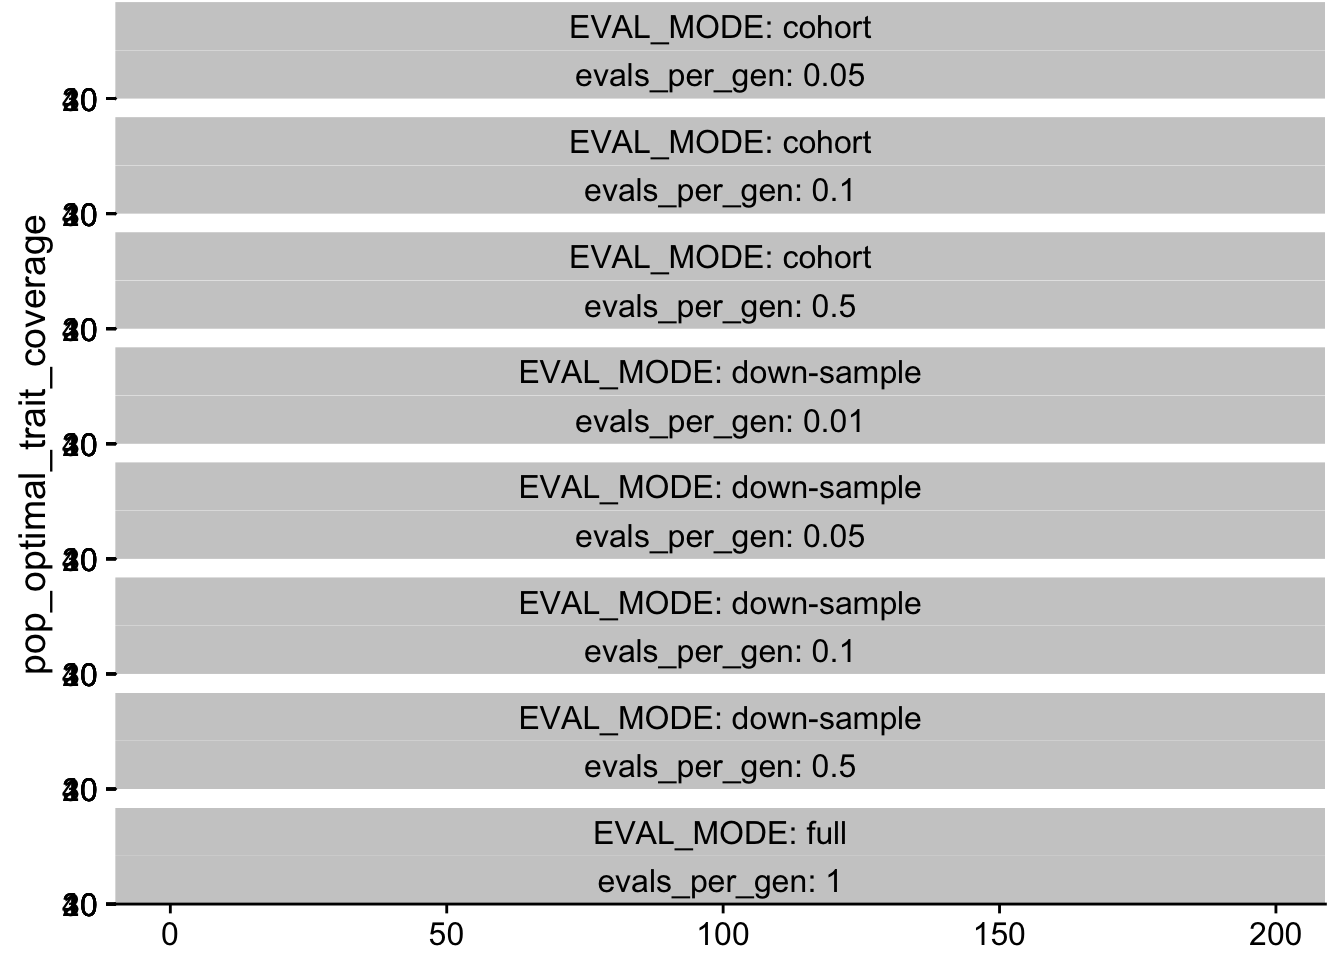
\includegraphics{phylogeny-informed-estimation-supplemental_files/figure-latex/unnamed-chunk-15-1.pdf}

\hypertarget{phylogeny-estimate-source-distributions}{%
\subsection{Phylogeny estimate source distributions}\label{phylogeny-estimate-source-distributions}}

\begin{Shaded}
\begin{Highlighting}[]
\NormalTok{est\_source\_data }\SpecialCharTok{\%\textgreater{}\%}
  \FunctionTok{filter}\NormalTok{(DIAGNOSTIC }\SpecialCharTok{==} \StringTok{"contradictory{-}objectives"}\NormalTok{) }\SpecialCharTok{\%\textgreater{}\%}
  \FunctionTok{filter}\NormalTok{(EVAL\_MODE }\SpecialCharTok{!=} \StringTok{"full"} \SpecialCharTok{\&}\NormalTok{ EVAL\_FIT\_EST\_MODE }\SpecialCharTok{!=} \StringTok{"None"}\NormalTok{) }\SpecialCharTok{\%\textgreater{}\%}
  \FunctionTok{ggplot}\NormalTok{(}
      \FunctionTok{aes}\NormalTok{(}
        \AttributeTok{x =}\NormalTok{ EVAL\_FIT\_EST\_MODE,}
        \AttributeTok{y =}\NormalTok{ prop\_self\_lookups}
\NormalTok{      )}
\NormalTok{    ) }\SpecialCharTok{+}
    \FunctionTok{geom\_boxplot}\NormalTok{() }\SpecialCharTok{+}
    \FunctionTok{geom\_point}\NormalTok{() }\SpecialCharTok{+}
    \FunctionTok{facet\_grid}\NormalTok{(}
      \AttributeTok{cols =} \FunctionTok{vars}\NormalTok{(evals\_per\_gen),}
      \AttributeTok{rows =} \FunctionTok{vars}\NormalTok{(EVAL\_MODE),}
      \AttributeTok{labeller =}\NormalTok{ label\_both}
\NormalTok{    ) }\SpecialCharTok{+}
    \FunctionTok{scale\_y\_continuous}\NormalTok{(}\StringTok{"Proportion of self lookups"}\NormalTok{) }\SpecialCharTok{+}
    \FunctionTok{scale\_x\_discrete}\NormalTok{(}\StringTok{"Evaluations per generation"}\NormalTok{) }\SpecialCharTok{+}
    \FunctionTok{theme\_bw}\NormalTok{() }\SpecialCharTok{+}
    \FunctionTok{theme}\NormalTok{(}\AttributeTok{legend.position =} \StringTok{"none"}\NormalTok{)}
\end{Highlighting}
\end{Shaded}

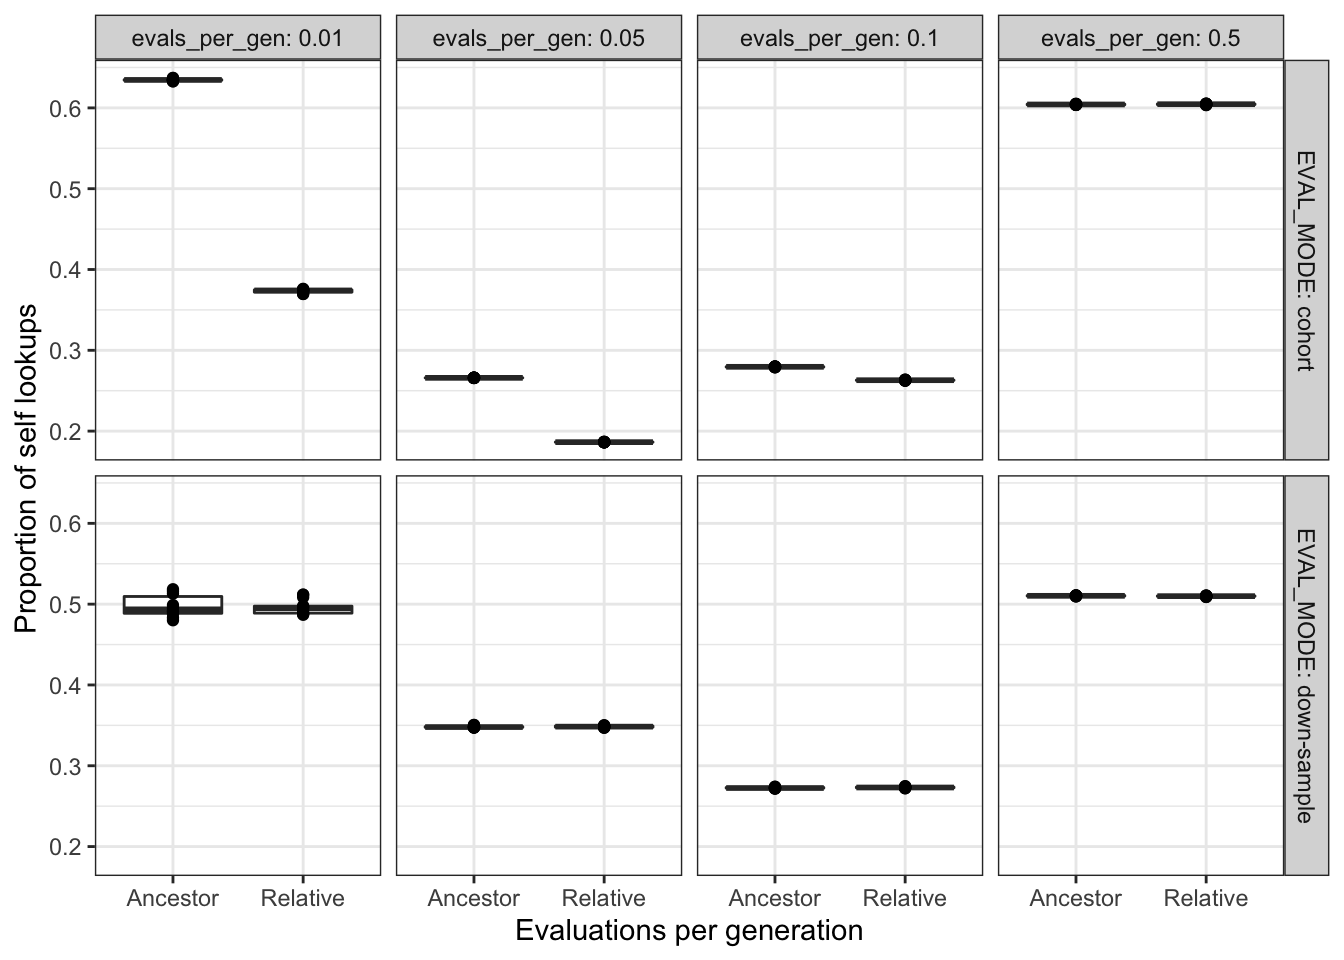
\includegraphics{phylogeny-informed-estimation-supplemental_files/figure-latex/unnamed-chunk-16-1.pdf}

\begin{Shaded}
\begin{Highlighting}[]
\FunctionTok{ggsave}\NormalTok{(}
   \AttributeTok{filename=}\FunctionTok{paste0}\NormalTok{(plot\_directory, }\StringTok{"contra{-}obj{-}self{-}lookups.pdf"}\NormalTok{)}
\NormalTok{)}
\end{Highlighting}
\end{Shaded}

\begin{verbatim}
## Saving 6.5 x 4.5 in image
\end{verbatim}

\begin{Shaded}
\begin{Highlighting}[]
\NormalTok{est\_source\_data }\SpecialCharTok{\%\textgreater{}\%}
  \FunctionTok{filter}\NormalTok{(DIAGNOSTIC }\SpecialCharTok{==} \StringTok{"contradictory{-}objectives"}\NormalTok{) }\SpecialCharTok{\%\textgreater{}\%}
  \FunctionTok{filter}\NormalTok{(EVAL\_MODE }\SpecialCharTok{!=} \StringTok{"full"} \SpecialCharTok{\&}\NormalTok{ EVAL\_FIT\_EST\_MODE }\SpecialCharTok{!=} \StringTok{"None"}\NormalTok{) }\SpecialCharTok{\%\textgreater{}\%}
  \FunctionTok{ggplot}\NormalTok{(}
      \FunctionTok{aes}\NormalTok{(}
        \AttributeTok{x =}\NormalTok{ EVAL\_FIT\_EST\_MODE,}
        \AttributeTok{y =}\NormalTok{ prop\_ancestor\_lookups}
\NormalTok{      )}
\NormalTok{    ) }\SpecialCharTok{+}
    \FunctionTok{geom\_boxplot}\NormalTok{() }\SpecialCharTok{+}
    \FunctionTok{geom\_point}\NormalTok{() }\SpecialCharTok{+}
    \FunctionTok{facet\_grid}\NormalTok{(}
      \AttributeTok{cols =} \FunctionTok{vars}\NormalTok{(evals\_per\_gen),}
      \AttributeTok{rows =} \FunctionTok{vars}\NormalTok{(EVAL\_MODE),}
      \AttributeTok{labeller =}\NormalTok{ label\_both}
\NormalTok{    ) }\SpecialCharTok{+}
    \FunctionTok{scale\_y\_continuous}\NormalTok{(}\StringTok{"Proportion of ancestor lookups"}\NormalTok{) }\SpecialCharTok{+}
    \FunctionTok{scale\_x\_discrete}\NormalTok{(}\StringTok{"Evaluations per generation"}\NormalTok{) }\SpecialCharTok{+}
    \FunctionTok{theme\_bw}\NormalTok{() }\SpecialCharTok{+}
    \FunctionTok{theme}\NormalTok{(}\AttributeTok{legend.position =} \StringTok{"none"}\NormalTok{)}
\end{Highlighting}
\end{Shaded}

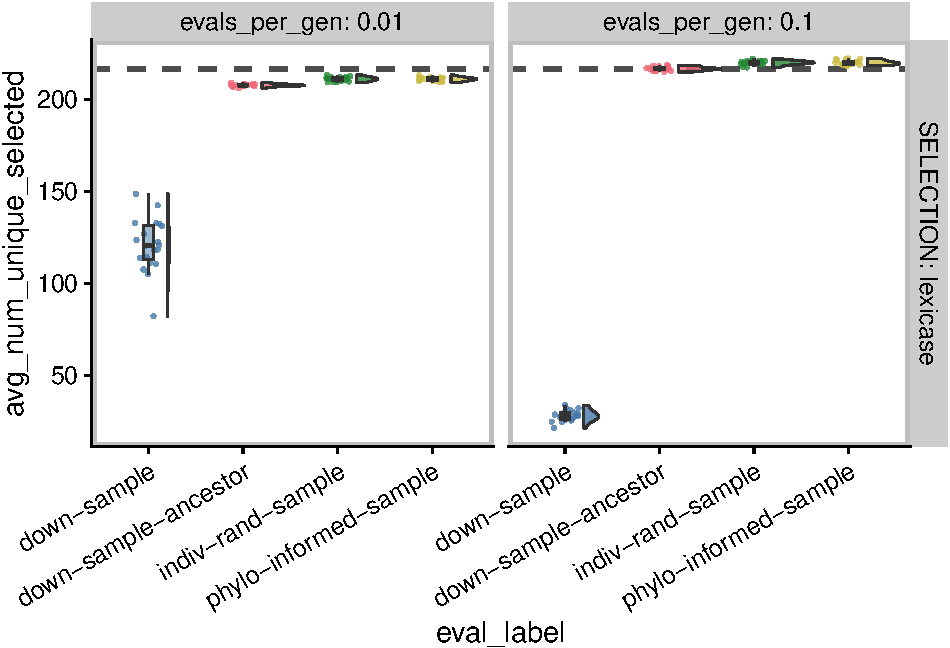
\includegraphics{phylogeny-informed-estimation-supplemental_files/figure-latex/unnamed-chunk-17-1.pdf}

\begin{Shaded}
\begin{Highlighting}[]
\FunctionTok{ggsave}\NormalTok{(}
   \AttributeTok{filename=}\FunctionTok{paste0}\NormalTok{(plot\_directory, }\StringTok{"contra{-}obj{-}ancestor{-}lookups.pdf"}\NormalTok{)}
\NormalTok{)}
\end{Highlighting}
\end{Shaded}

\begin{verbatim}
## Saving 6.5 x 4.5 in image
\end{verbatim}

\begin{Shaded}
\begin{Highlighting}[]
\NormalTok{est\_source\_data }\SpecialCharTok{\%\textgreater{}\%}
  \FunctionTok{filter}\NormalTok{(DIAGNOSTIC }\SpecialCharTok{==} \StringTok{"contradictory{-}objectives"}\NormalTok{) }\SpecialCharTok{\%\textgreater{}\%}
  \FunctionTok{filter}\NormalTok{(EVAL\_MODE }\SpecialCharTok{!=} \StringTok{"full"} \SpecialCharTok{\&}\NormalTok{ EVAL\_FIT\_EST\_MODE }\SpecialCharTok{!=} \StringTok{"None"}\NormalTok{) }\SpecialCharTok{\%\textgreater{}\%}
  \FunctionTok{ggplot}\NormalTok{(}
      \FunctionTok{aes}\NormalTok{(}
        \AttributeTok{x =}\NormalTok{ EVAL\_FIT\_EST\_MODE,}
        \AttributeTok{y =}\NormalTok{ prop\_descendant\_lookups}
\NormalTok{      )}
\NormalTok{    ) }\SpecialCharTok{+}
    \FunctionTok{geom\_boxplot}\NormalTok{() }\SpecialCharTok{+}
    \FunctionTok{geom\_point}\NormalTok{() }\SpecialCharTok{+}
    \FunctionTok{facet\_grid}\NormalTok{(}
      \AttributeTok{cols =} \FunctionTok{vars}\NormalTok{(evals\_per\_gen),}
      \AttributeTok{rows =} \FunctionTok{vars}\NormalTok{(EVAL\_MODE),}
      \AttributeTok{labeller =}\NormalTok{ label\_both}
\NormalTok{    ) }\SpecialCharTok{+}
    \FunctionTok{scale\_y\_continuous}\NormalTok{(}\StringTok{"Proportion of descendant lookups"}\NormalTok{) }\SpecialCharTok{+}
    \FunctionTok{scale\_x\_discrete}\NormalTok{(}\StringTok{"Evaluations per generation"}\NormalTok{) }\SpecialCharTok{+}
    \FunctionTok{theme\_bw}\NormalTok{() }\SpecialCharTok{+}
    \FunctionTok{theme}\NormalTok{(}\AttributeTok{legend.position =} \StringTok{"none"}\NormalTok{)}
\end{Highlighting}
\end{Shaded}

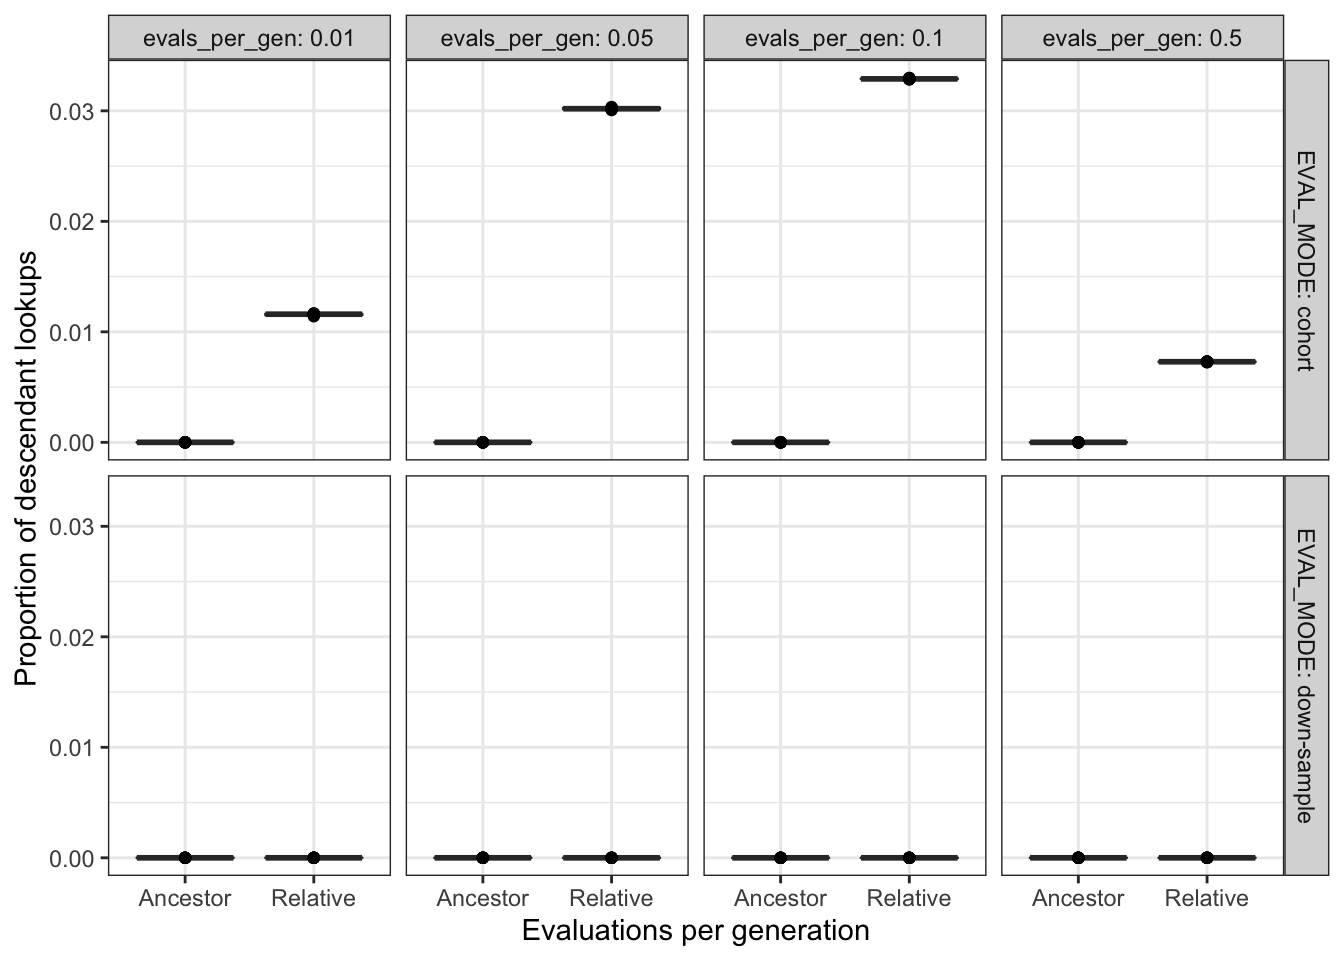
\includegraphics{phylogeny-informed-estimation-supplemental_files/figure-latex/unnamed-chunk-18-1.pdf}

\begin{Shaded}
\begin{Highlighting}[]
\FunctionTok{ggsave}\NormalTok{(}
   \AttributeTok{filename=}\FunctionTok{paste0}\NormalTok{(plot\_directory, }\StringTok{"contra{-}obj{-}descendant{-}lookups.pdf"}\NormalTok{)}
\NormalTok{)}
\end{Highlighting}
\end{Shaded}

\begin{verbatim}
## Saving 6.5 x 4.5 in image
\end{verbatim}

\begin{Shaded}
\begin{Highlighting}[]
\NormalTok{est\_source\_data }\SpecialCharTok{\%\textgreater{}\%}
  \FunctionTok{filter}\NormalTok{(DIAGNOSTIC }\SpecialCharTok{==} \StringTok{"contradictory{-}objectives"}\NormalTok{) }\SpecialCharTok{\%\textgreater{}\%}
  \FunctionTok{filter}\NormalTok{(EVAL\_MODE }\SpecialCharTok{!=} \StringTok{"full"} \SpecialCharTok{\&}\NormalTok{ EVAL\_FIT\_EST\_MODE }\SpecialCharTok{!=} \StringTok{"None"}\NormalTok{) }\SpecialCharTok{\%\textgreater{}\%}
  \FunctionTok{ggplot}\NormalTok{(}
      \FunctionTok{aes}\NormalTok{(}
        \AttributeTok{x =}\NormalTok{ EVAL\_FIT\_EST\_MODE,}
        \AttributeTok{y =}\NormalTok{ prop\_other\_lookups}
\NormalTok{      )}
\NormalTok{    ) }\SpecialCharTok{+}
    \FunctionTok{geom\_boxplot}\NormalTok{() }\SpecialCharTok{+}
    \FunctionTok{geom\_point}\NormalTok{() }\SpecialCharTok{+}
    \FunctionTok{facet\_grid}\NormalTok{(}
      \AttributeTok{cols =} \FunctionTok{vars}\NormalTok{(evals\_per\_gen),}
      \AttributeTok{rows =} \FunctionTok{vars}\NormalTok{(EVAL\_MODE),}
      \AttributeTok{labeller =}\NormalTok{ label\_both}
\NormalTok{    ) }\SpecialCharTok{+}
    \FunctionTok{scale\_y\_continuous}\NormalTok{(}\StringTok{"Proportion of other lookups"}\NormalTok{) }\SpecialCharTok{+}
    \FunctionTok{scale\_x\_discrete}\NormalTok{(}\StringTok{"Evaluations per generation"}\NormalTok{) }\SpecialCharTok{+}
    \FunctionTok{theme\_bw}\NormalTok{() }\SpecialCharTok{+}
    \FunctionTok{theme}\NormalTok{(}\AttributeTok{legend.position =} \StringTok{"none"}\NormalTok{)}
\end{Highlighting}
\end{Shaded}

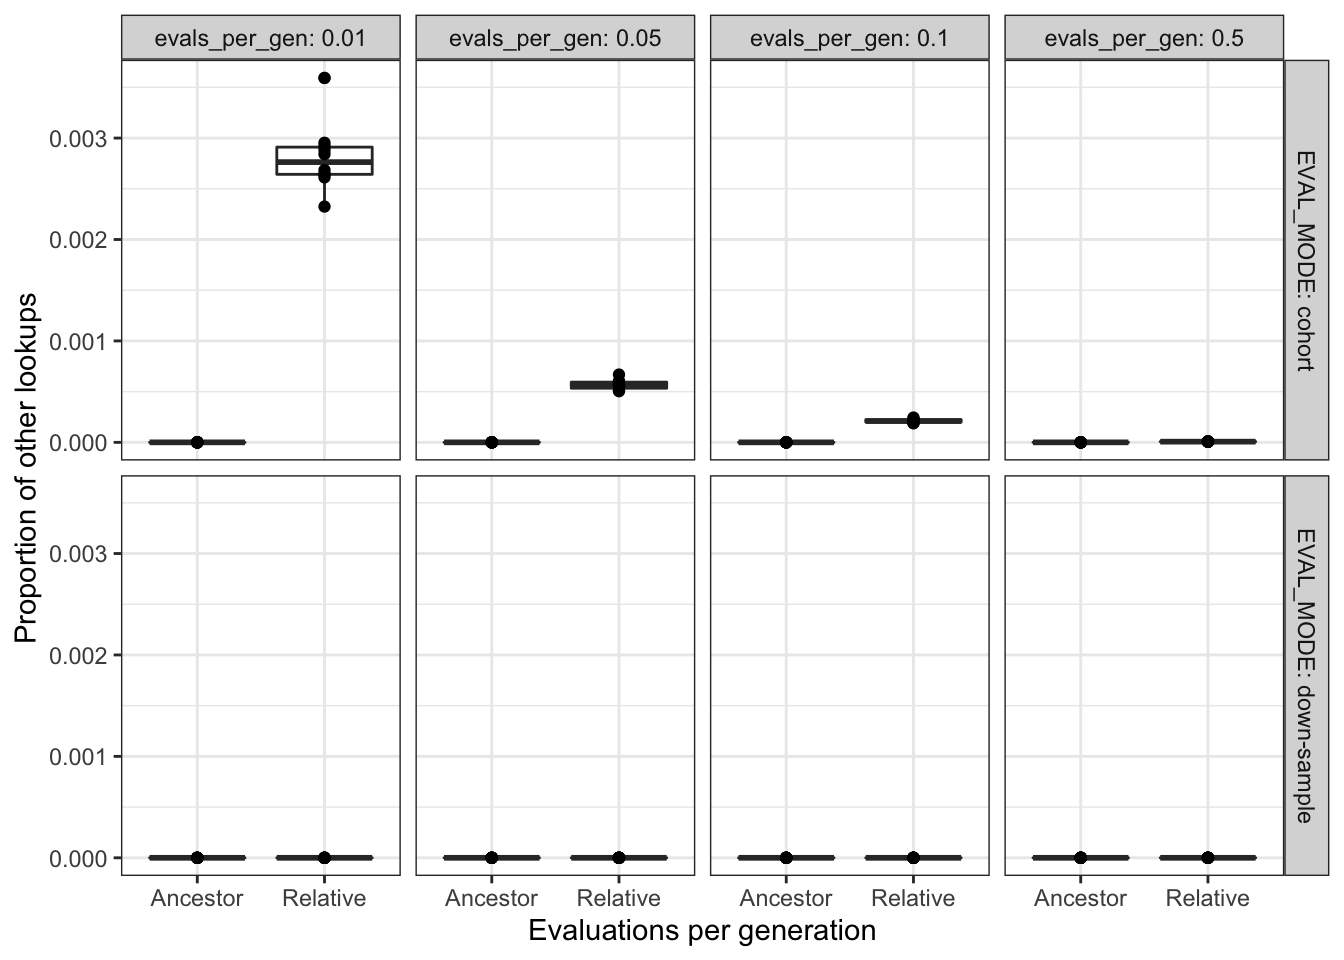
\includegraphics{phylogeny-informed-estimation-supplemental_files/figure-latex/unnamed-chunk-19-1.pdf}

\begin{Shaded}
\begin{Highlighting}[]
\FunctionTok{ggsave}\NormalTok{(}
   \AttributeTok{filename=}\FunctionTok{paste0}\NormalTok{(plot\_directory, }\StringTok{"contra{-}obj{-}other{-}lookups.pdf"}\NormalTok{)}
\NormalTok{)}
\end{Highlighting}
\end{Shaded}

\begin{verbatim}
## Saving 6.5 x 4.5 in image
\end{verbatim}

\begin{Shaded}
\begin{Highlighting}[]
\NormalTok{est\_source\_data }\SpecialCharTok{\%\textgreater{}\%}
  \FunctionTok{filter}\NormalTok{(DIAGNOSTIC }\SpecialCharTok{==} \StringTok{"contradictory{-}objectives"}\NormalTok{) }\SpecialCharTok{\%\textgreater{}\%}
  \FunctionTok{filter}\NormalTok{(EVAL\_MODE }\SpecialCharTok{!=} \StringTok{"full"} \SpecialCharTok{\&}\NormalTok{ EVAL\_FIT\_EST\_MODE }\SpecialCharTok{!=} \StringTok{"None"}\NormalTok{) }\SpecialCharTok{\%\textgreater{}\%}
  \FunctionTok{ggplot}\NormalTok{(}
      \FunctionTok{aes}\NormalTok{(}
        \AttributeTok{x =}\NormalTok{ EVAL\_FIT\_EST\_MODE,}
        \AttributeTok{y =}\NormalTok{ prop\_outside\_lookups}
\NormalTok{      )}
\NormalTok{    ) }\SpecialCharTok{+}
    \FunctionTok{geom\_boxplot}\NormalTok{() }\SpecialCharTok{+}
    \FunctionTok{geom\_point}\NormalTok{() }\SpecialCharTok{+}
    \FunctionTok{facet\_grid}\NormalTok{(}
      \AttributeTok{cols =} \FunctionTok{vars}\NormalTok{(evals\_per\_gen),}
      \AttributeTok{rows =} \FunctionTok{vars}\NormalTok{(EVAL\_MODE),}
      \AttributeTok{labeller =}\NormalTok{ label\_both}
\NormalTok{    ) }\SpecialCharTok{+}
    \FunctionTok{scale\_y\_continuous}\NormalTok{(}\StringTok{"Proportion of outside lookups"}\NormalTok{) }\SpecialCharTok{+}
    \FunctionTok{scale\_x\_discrete}\NormalTok{(}\StringTok{"Evaluations per generation"}\NormalTok{) }\SpecialCharTok{+}
    \FunctionTok{theme\_bw}\NormalTok{() }\SpecialCharTok{+}
    \FunctionTok{theme}\NormalTok{(}\AttributeTok{legend.position =} \StringTok{"none"}\NormalTok{)}
\end{Highlighting}
\end{Shaded}

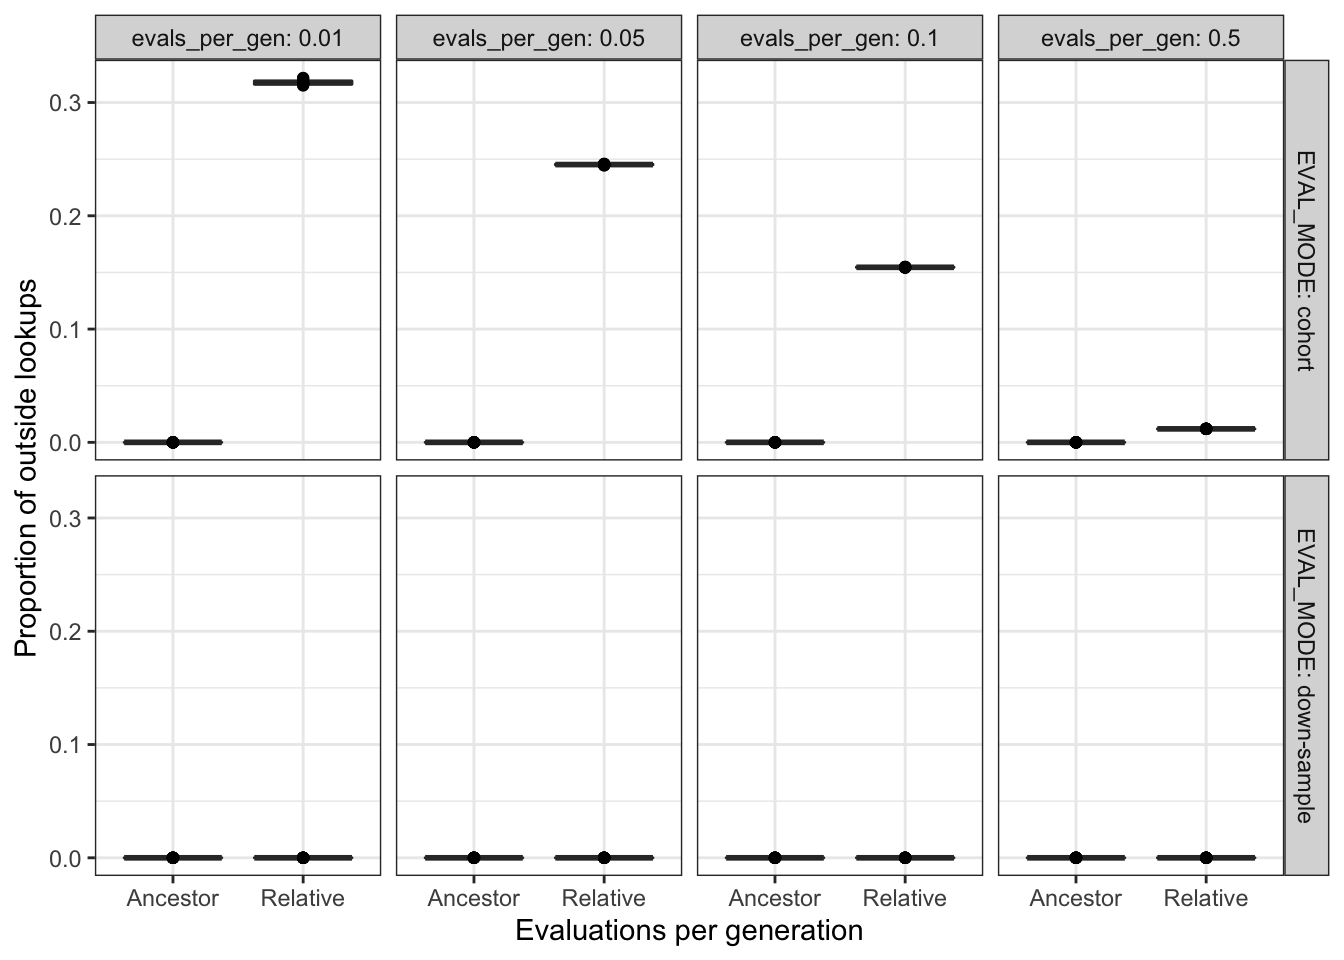
\includegraphics{phylogeny-informed-estimation-supplemental_files/figure-latex/unnamed-chunk-20-1.pdf}

\begin{Shaded}
\begin{Highlighting}[]
\FunctionTok{ggsave}\NormalTok{(}
   \AttributeTok{filename=}\FunctionTok{paste0}\NormalTok{(plot\_directory, }\StringTok{"contra{-}obj{-}outside{-}lookups.pdf"}\NormalTok{)}
\NormalTok{)}
\end{Highlighting}
\end{Shaded}

\begin{verbatim}
## Saving 6.5 x 4.5 in image
\end{verbatim}

\hypertarget{multi-path-exploration-diagnostic}{%
\section{Multi-path exploration diagnostic}\label{multi-path-exploration-diagnostic}}

\hypertarget{maximum-aggregate-score-final}{%
\subsection{Maximum aggregate score (final)}\label{maximum-aggregate-score-final}}

\begin{Shaded}
\begin{Highlighting}[]
\NormalTok{explore\_final\_score\_plt }\OtherTok{\textless{}{-}} \FunctionTok{ggplot}\NormalTok{(}
\NormalTok{    explore\_summary\_data,}
    \FunctionTok{aes}\NormalTok{(}
      \AttributeTok{x =}\NormalTok{ EVAL\_FIT\_EST\_MODE,}
      \AttributeTok{y =}\NormalTok{ max\_agg\_score,}
      \AttributeTok{fill =}\NormalTok{ EVAL\_FIT\_EST\_MODE}
\NormalTok{    )}
\NormalTok{  ) }\SpecialCharTok{+}
  \FunctionTok{geom\_flat\_violin}\NormalTok{(}
    \AttributeTok{position =} \FunctionTok{position\_nudge}\NormalTok{(}\AttributeTok{x =}\NormalTok{ .}\DecValTok{2}\NormalTok{, }\AttributeTok{y =} \DecValTok{0}\NormalTok{),}
    \AttributeTok{alpha =}\NormalTok{ .}\DecValTok{8}\NormalTok{,}
    \AttributeTok{adjust=}\FloatTok{1.5}
\NormalTok{  ) }\SpecialCharTok{+}
  \FunctionTok{geom\_point}\NormalTok{(}
    \AttributeTok{mapping=}\FunctionTok{aes}\NormalTok{(}\AttributeTok{color=}\NormalTok{EVAL\_FIT\_EST\_MODE),}
    \AttributeTok{position =} \FunctionTok{position\_jitter}\NormalTok{(}\AttributeTok{width =}\NormalTok{ .}\DecValTok{15}\NormalTok{),}
    \AttributeTok{size =}\NormalTok{ .}\DecValTok{5}\NormalTok{,}
    \AttributeTok{alpha =} \FloatTok{0.8}
\NormalTok{  ) }\SpecialCharTok{+}
  \FunctionTok{geom\_boxplot}\NormalTok{(}
    \AttributeTok{width =}\NormalTok{ .}\DecValTok{1}\NormalTok{,}
    \AttributeTok{outlier.shape =} \ConstantTok{NA}\NormalTok{,}
    \AttributeTok{alpha =} \FloatTok{0.5}
\NormalTok{  ) }\SpecialCharTok{+}
  \FunctionTok{scale\_y\_continuous}\NormalTok{(}
    \CommentTok{\# limits = c({-}0.5, 100)}
\NormalTok{  ) }\SpecialCharTok{+}
  \FunctionTok{scale\_fill\_bright}\NormalTok{() }\SpecialCharTok{+}
  \FunctionTok{scale\_color\_bright}\NormalTok{() }\SpecialCharTok{+}
  \FunctionTok{facet\_grid}\NormalTok{(}
\NormalTok{    eval\_mode\_row}\SpecialCharTok{\textasciitilde{}}\NormalTok{evals\_per\_gen,}
    \CommentTok{\# nrow=2,}
    \AttributeTok{labeller=}\NormalTok{label\_both}
\NormalTok{  ) }\SpecialCharTok{+}
  \FunctionTok{theme}\NormalTok{(}
    \AttributeTok{legend.position =} \StringTok{"none"}\NormalTok{,}
    \AttributeTok{axis.text.x =} \FunctionTok{element\_text}\NormalTok{(}
      \AttributeTok{angle =} \DecValTok{30}\NormalTok{,}
      \AttributeTok{hjust =} \DecValTok{1}
\NormalTok{    ),}
    \AttributeTok{panel.border =} \FunctionTok{element\_rect}\NormalTok{(}\AttributeTok{color=}\StringTok{"gray"}\NormalTok{, }\AttributeTok{size=}\DecValTok{2}\NormalTok{)}
\NormalTok{  )}
\FunctionTok{ggsave}\NormalTok{(}
  \AttributeTok{filename =} \FunctionTok{paste0}\NormalTok{(plot\_directory, }\StringTok{"explore{-}final.pdf"}\NormalTok{),}
  \AttributeTok{plot =}\NormalTok{ explore\_final\_score\_plt }\SpecialCharTok{+} \FunctionTok{labs}\NormalTok{(}\AttributeTok{title=}\StringTok{"Multi{-}path exploration"}\NormalTok{),}
  \AttributeTok{width =} \DecValTok{15}\NormalTok{,}
  \AttributeTok{height =} \DecValTok{10}
\NormalTok{)}
\end{Highlighting}
\end{Shaded}

\hypertarget{statistical-analysis-1}{%
\subsubsection{Statistical analysis}\label{statistical-analysis-1}}

\begin{Shaded}
\begin{Highlighting}[]
\NormalTok{explore\_summary\_data }\SpecialCharTok{\%\textgreater{}\%}
  \FunctionTok{filter}\NormalTok{(EVAL\_MODE }\SpecialCharTok{!=} \StringTok{"full"}\NormalTok{) }\SpecialCharTok{\%\textgreater{}\%}
  \FunctionTok{group\_by}\NormalTok{(EVAL\_MODE, evals\_per\_gen, EVAL\_FIT\_EST\_MODE) }\SpecialCharTok{\%\textgreater{}\%}
  \FunctionTok{summarize}\NormalTok{(}
    \AttributeTok{score\_median =} \FunctionTok{median}\NormalTok{(max\_agg\_score),}
    \AttributeTok{score\_mean =} \FunctionTok{mean}\NormalTok{(max\_agg\_score),}
    \AttributeTok{n =} \FunctionTok{n}\NormalTok{()}
\NormalTok{  ) }\SpecialCharTok{\%\textgreater{}\%}
  \FunctionTok{kable}\NormalTok{()}
\end{Highlighting}
\end{Shaded}

\begin{verbatim}
## `summarise()` has grouped output by 'EVAL_MODE', 'evals_per_gen'. You can
## override using the `.groups` argument.
\end{verbatim}

\begin{tabular}{l|l|l|r|r|r}
\hline
EVAL\_MODE & evals\_per\_gen & EVAL\_FIT\_EST\_MODE & score\_median & score\_mean & n\\
\hline
cohort & 0.01 & None & 1971.7450 & 1900.3130 & 10\\
\hline
cohort & 0.01 & Ancestor & 2316.5800 & 1971.5663 & 10\\
\hline
cohort & 0.01 & Relative & 2182.5700 & 2006.6843 & 10\\
\hline
cohort & 0.05 & None & 2401.0150 & 2373.2040 & 10\\
\hline
cohort & 0.05 & Ancestor & 2858.6950 & 2747.0960 & 10\\
\hline
cohort & 0.05 & Relative & 3471.8500 & 3389.0910 & 10\\
\hline
cohort & 0.1 & None & 3075.5150 & 3076.6120 & 10\\
\hline
cohort & 0.1 & Ancestor & 4508.1150 & 4383.9440 & 10\\
\hline
cohort & 0.1 & Relative & 5144.5350 & 5163.0130 & 10\\
\hline
cohort & 0.5 & None & 8187.5000 & 8198.1150 & 10\\
\hline
cohort & 0.5 & Ancestor & 8591.7150 & 8708.0110 & 10\\
\hline
cohort & 0.5 & Relative & 8684.2050 & 8652.1500 & 10\\
\hline
down-sample & 0.01 & None & 580.4215 & 532.1152 & 10\\
\hline
down-sample & 0.01 & Ancestor & 434.8545 & 430.0114 & 10\\
\hline
down-sample & 0.01 & Relative & 449.3640 & 465.0957 & 10\\
\hline
down-sample & 0.05 & None & 396.0890 & 445.1163 & 10\\
\hline
down-sample & 0.05 & Ancestor & 2007.3700 & 1982.4690 & 10\\
\hline
down-sample & 0.05 & Relative & 1777.9000 & 1762.3250 & 10\\
\hline
down-sample & 0.1 & None & 692.7270 & 690.7322 & 10\\
\hline
down-sample & 0.1 & Ancestor & 2423.2200 & 2451.7950 & 10\\
\hline
down-sample & 0.1 & Relative & 2529.6100 & 2542.1340 & 10\\
\hline
down-sample & 0.5 & None & 1499.9800 & 1658.0837 & 10\\
\hline
down-sample & 0.5 & Ancestor & 6976.5950 & 6972.2630 & 10\\
\hline
down-sample & 0.5 & Relative & 7309.9450 & 7120.4160 & 10\\
\hline
\end{tabular}

\begin{Shaded}
\begin{Highlighting}[]
\NormalTok{explore\_kw\_test }\OtherTok{\textless{}{-}}\NormalTok{ explore\_summary\_data }\SpecialCharTok{\%\textgreater{}\%}
  \FunctionTok{filter}\NormalTok{(EVAL\_MODE }\SpecialCharTok{!=} \StringTok{"full"}\NormalTok{) }\SpecialCharTok{\%\textgreater{}\%}
  \FunctionTok{group\_by}\NormalTok{(EVAL\_MODE, evals\_per\_gen) }\SpecialCharTok{\%\textgreater{}\%}
  \FunctionTok{kruskal\_test}\NormalTok{(max\_agg\_score }\SpecialCharTok{\textasciitilde{}}\NormalTok{ EVAL\_FIT\_EST\_MODE) }\SpecialCharTok{\%\textgreater{}\%}
  \FunctionTok{mutate}\NormalTok{(}
    \AttributeTok{sig =}\NormalTok{ (p }\SpecialCharTok{\textless{}=} \FloatTok{0.05}\NormalTok{)}
\NormalTok{  ) }\SpecialCharTok{\%\textgreater{}\%}
  \FunctionTok{unite}\NormalTok{(}
    \StringTok{"comparison\_group"}\NormalTok{,}
\NormalTok{    EVAL\_MODE,}
\NormalTok{    evals\_per\_gen,}
    \AttributeTok{sep =} \StringTok{"\_"}\NormalTok{,}
    \AttributeTok{remove =} \ConstantTok{FALSE}
\NormalTok{  )}

\FunctionTok{kable}\NormalTok{(explore\_kw\_test)}
\end{Highlighting}
\end{Shaded}

\begin{tabular}{l|l|l|l|r|r|r|r|l|l}
\hline
comparison\_group & EVAL\_MODE & evals\_per\_gen & .y. & n & statistic & df & p & method & sig\\
\hline
cohort\_0.01 & cohort & 0.01 & max\_agg\_score & 30 & 0.7045161 & 2 & 7.03e-01 & Kruskal-Wallis & FALSE\\
\hline
cohort\_0.05 & cohort & 0.05 & max\_agg\_score & 30 & 15.5380645 & 2 & 4.23e-04 & Kruskal-Wallis & TRUE\\
\hline
cohort\_0.1 & cohort & 0.1 & max\_agg\_score & 30 & 25.5509677 & 2 & 2.80e-06 & Kruskal-Wallis & TRUE\\
\hline
cohort\_0.5 & cohort & 0.5 & max\_agg\_score & 30 & 5.0348387 & 2 & 8.07e-02 & Kruskal-Wallis & FALSE\\
\hline
down-sample\_0.01 & down-sample & 0.01 & max\_agg\_score & 30 & 2.6090323 & 2 & 2.71e-01 & Kruskal-Wallis & FALSE\\
\hline
down-sample\_0.05 & down-sample & 0.05 & max\_agg\_score & 30 & 22.3380645 & 2 & 1.41e-05 & Kruskal-Wallis & TRUE\\
\hline
down-sample\_0.1 & down-sample & 0.1 & max\_agg\_score & 30 & 19.3780645 & 2 & 6.20e-05 & Kruskal-Wallis & TRUE\\
\hline
down-sample\_0.5 & down-sample & 0.5 & max\_agg\_score & 30 & 19.4047630 & 2 & 6.11e-05 & Kruskal-Wallis & TRUE\\
\hline
\end{tabular}

\begin{Shaded}
\begin{Highlighting}[]
\NormalTok{expl\_sig\_kw\_groups }\OtherTok{\textless{}{-}} \FunctionTok{filter}\NormalTok{(explore\_kw\_test, p }\SpecialCharTok{\textless{}} \FloatTok{0.05}\NormalTok{)}\SpecialCharTok{$}\NormalTok{comparison\_group}

\NormalTok{explore\_stats }\OtherTok{\textless{}{-}}\NormalTok{ explore\_summary\_data }\SpecialCharTok{\%\textgreater{}\%}
  \FunctionTok{unite}\NormalTok{(}
    \StringTok{"comparison\_group"}\NormalTok{,}
\NormalTok{    EVAL\_MODE,}
\NormalTok{    evals\_per\_gen,}
    \AttributeTok{sep =} \StringTok{"\_"}\NormalTok{,}
    \AttributeTok{remove =} \ConstantTok{FALSE}
\NormalTok{  ) }\SpecialCharTok{\%\textgreater{}\%}
  \FunctionTok{filter}\NormalTok{(EVAL\_MODE }\SpecialCharTok{!=} \StringTok{"full"} \SpecialCharTok{\&}\NormalTok{ comparison\_group }\SpecialCharTok{\%in\%}\NormalTok{ expl\_sig\_kw\_groups) }\SpecialCharTok{\%\textgreater{}\%}
  \FunctionTok{group\_by}\NormalTok{(EVAL\_MODE, evals\_per\_gen) }\SpecialCharTok{\%\textgreater{}\%}
  \FunctionTok{pairwise\_wilcox\_test}\NormalTok{(max\_agg\_score }\SpecialCharTok{\textasciitilde{}}\NormalTok{ EVAL\_FIT\_EST\_MODE) }\SpecialCharTok{\%\textgreater{}\%}
  \FunctionTok{adjust\_pvalue}\NormalTok{(}\AttributeTok{method =} \StringTok{"holm"}\NormalTok{) }\SpecialCharTok{\%\textgreater{}\%}
  \FunctionTok{add\_significance}\NormalTok{(}\StringTok{"p.adj"}\NormalTok{)}

\FunctionTok{kable}\NormalTok{(explore\_stats)}
\end{Highlighting}
\end{Shaded}

\begin{tabular}{l|l|l|l|l|r|r|r|r|r|l}
\hline
EVAL\_MODE & evals\_per\_gen & .y. & group1 & group2 & n1 & n2 & statistic & p & p.adj & p.adj.signif\\
\hline
cohort & 0.05 & max\_agg\_score & None & Ancestor & 10 & 10 & 27 & 8.90e-02 & 0.2670000 & ns\\
\hline
cohort & 0.05 & max\_agg\_score & None & Relative & 10 & 10 & 4 & 1.30e-04 & 0.0010400 & **\\
\hline
cohort & 0.05 & max\_agg\_score & Ancestor & Relative & 10 & 10 & 12 & 3.00e-03 & 0.0150000 & *\\
\hline
cohort & 0.1 & max\_agg\_score & None & Ancestor & 10 & 10 & 0 & 1.08e-05 & 0.0001620 & ***\\
\hline
cohort & 0.1 & max\_agg\_score & None & Relative & 10 & 10 & 0 & 1.08e-05 & 0.0001620 & ***\\
\hline
cohort & 0.1 & max\_agg\_score & Ancestor & Relative & 10 & 10 & 1 & 2.17e-05 & 0.0001953 & ***\\
\hline
down-sample & 0.05 & max\_agg\_score & None & Ancestor & 10 & 10 & 0 & 1.08e-05 & 0.0001620 & ***\\
\hline
down-sample & 0.05 & max\_agg\_score & None & Relative & 10 & 10 & 0 & 1.08e-05 & 0.0001620 & ***\\
\hline
down-sample & 0.05 & max\_agg\_score & Ancestor & Relative & 10 & 10 & 84 & 9.00e-03 & 0.0360000 & *\\
\hline
down-sample & 0.1 & max\_agg\_score & None & Ancestor & 10 & 10 & 0 & 1.08e-05 & 0.0001620 & ***\\
\hline
down-sample & 0.1 & max\_agg\_score & None & Relative & 10 & 10 & 0 & 1.08e-05 & 0.0001620 & ***\\
\hline
down-sample & 0.1 & max\_agg\_score & Ancestor & Relative & 10 & 10 & 47 & 8.53e-01 & 1.0000000 & ns\\
\hline
down-sample & 0.5 & max\_agg\_score & None & Ancestor & 10 & 10 & 0 & 1.81e-04 & 0.0012670 & **\\
\hline
down-sample & 0.5 & max\_agg\_score & None & Relative & 10 & 10 & 0 & 1.81e-04 & 0.0012670 & **\\
\hline
down-sample & 0.5 & max\_agg\_score & Ancestor & Relative & 10 & 10 & 46 & 7.96e-01 & 1.0000000 & ns\\
\hline
\end{tabular}

\begin{Shaded}
\begin{Highlighting}[]
\CommentTok{\# explore\_stats \%\textgreater{}\%}
\CommentTok{\#   filter(p.adj \textless{}= 0.05) \%\textgreater{}\%}
\CommentTok{\#   arrange(}
\CommentTok{\#     desc(p.adj)}
\CommentTok{\#   ) \%\textgreater{}\%}
\CommentTok{\#   kable()}
\end{Highlighting}
\end{Shaded}

\hypertarget{maximum-aggregate-score-over-time}{%
\subsection{Maximum aggregate score (over time)}\label{maximum-aggregate-score-over-time}}

\begin{Shaded}
\begin{Highlighting}[]
\NormalTok{explore\_score\_ts }\OtherTok{\textless{}{-}} \FunctionTok{ggplot}\NormalTok{(}
\NormalTok{    explore\_ts\_data,}
    \FunctionTok{aes}\NormalTok{(}
      \AttributeTok{x =}\NormalTok{ ts\_step,}
      \AttributeTok{y =}\NormalTok{ max\_agg\_score,}
      \AttributeTok{fill =}\NormalTok{ EVAL\_FIT\_EST\_MODE,}
      \AttributeTok{color =}\NormalTok{ EVAL\_FIT\_EST\_MODE}
\NormalTok{    )}
\NormalTok{  ) }\SpecialCharTok{+}
  \FunctionTok{stat\_summary}\NormalTok{(}
    \AttributeTok{geom =} \StringTok{"line"}\NormalTok{,}
    \AttributeTok{fun =}\NormalTok{ mean}
\NormalTok{  ) }\SpecialCharTok{+}
  \FunctionTok{stat\_summary}\NormalTok{(}
    \AttributeTok{geom =} \StringTok{"ribbon"}\NormalTok{,}
    \AttributeTok{fun.data =} \StringTok{"mean\_cl\_boot"}\NormalTok{,}
    \AttributeTok{fun.args =} \FunctionTok{list}\NormalTok{(}\AttributeTok{conf.int =} \FloatTok{0.95}\NormalTok{),}
    \AttributeTok{alpha =} \FloatTok{0.2}\NormalTok{,}
    \AttributeTok{linetype =} \DecValTok{0}
\NormalTok{  ) }\SpecialCharTok{+}
  \FunctionTok{scale\_fill\_bright}\NormalTok{() }\SpecialCharTok{+}
  \FunctionTok{scale\_color\_bright}\NormalTok{() }\SpecialCharTok{+}
  \FunctionTok{facet\_wrap}\NormalTok{(}
\NormalTok{    EVAL\_MODE }\SpecialCharTok{\textasciitilde{}}\NormalTok{ evals\_per\_gen,}
    \AttributeTok{ncol =} \DecValTok{1}\NormalTok{,}
    \AttributeTok{labeller =}\NormalTok{ label\_both}
\NormalTok{  ) }\SpecialCharTok{+}
  \FunctionTok{theme}\NormalTok{(}
    \AttributeTok{legend.position =} \StringTok{"bottom"}
\NormalTok{  )}

\FunctionTok{ggsave}\NormalTok{(}
  \AttributeTok{filename =} \FunctionTok{paste0}\NormalTok{(plot\_directory, }\StringTok{"explore{-}ts.pdf"}\NormalTok{),}
  \AttributeTok{plot =}\NormalTok{ explore\_score\_ts }\SpecialCharTok{+} \FunctionTok{labs}\NormalTok{(}\AttributeTok{title=}\StringTok{"Multi{-}path exploration"}\NormalTok{),}
  \AttributeTok{width =} \DecValTok{10}\NormalTok{,}
  \AttributeTok{height =} \DecValTok{15}
\NormalTok{)}
\end{Highlighting}
\end{Shaded}

\begin{Shaded}
\begin{Highlighting}[]
\NormalTok{explore\_score\_ts}
\end{Highlighting}
\end{Shaded}

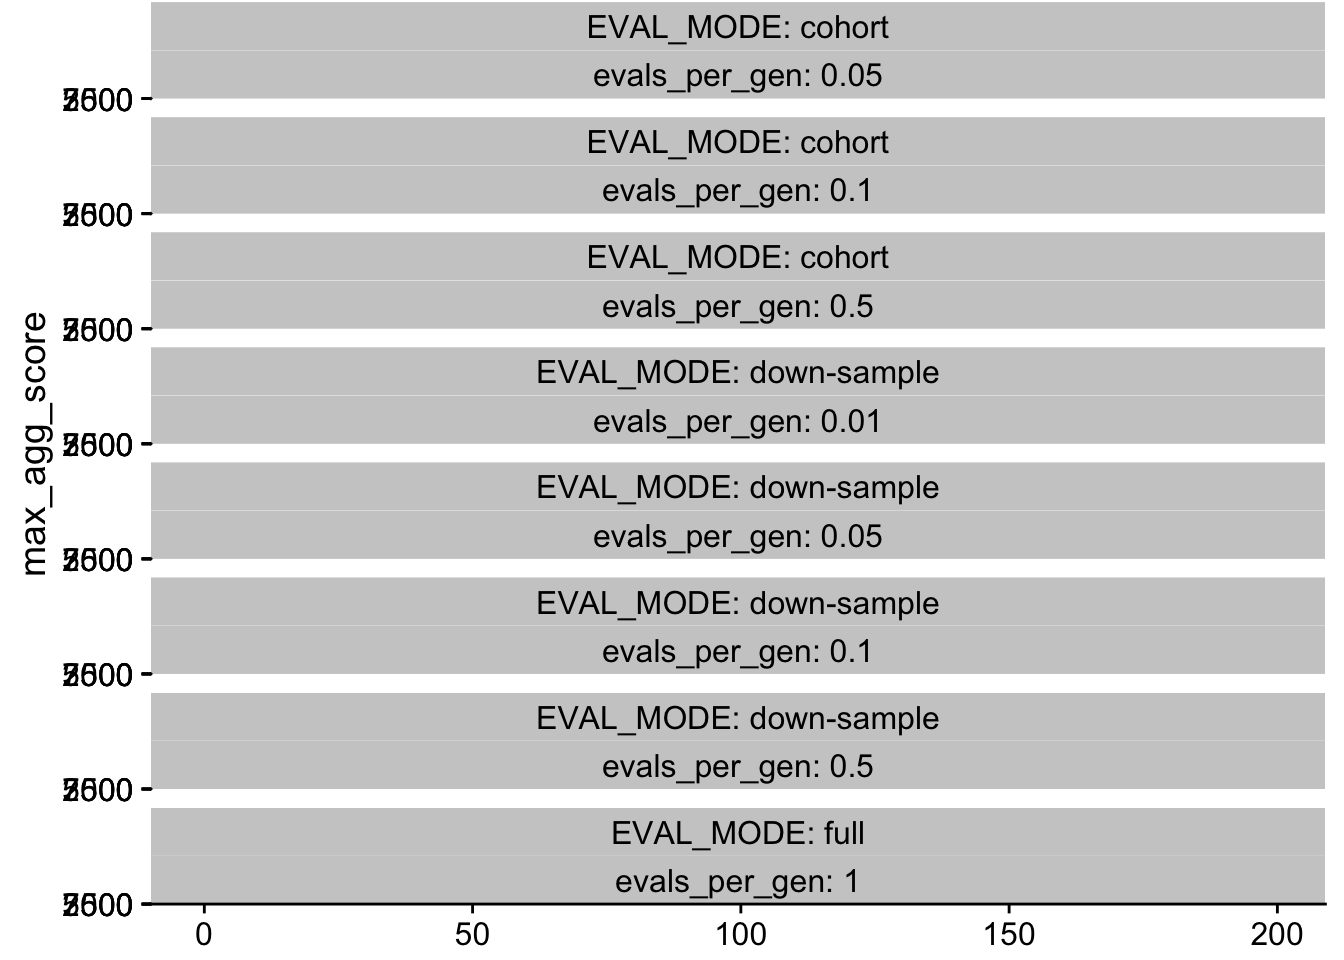
\includegraphics{phylogeny-informed-estimation-supplemental_files/figure-latex/unnamed-chunk-26-1.pdf}

\hypertarget{phylogeny-estimate-source-distributions-1}{%
\subsection{Phylogeny estimate source distributions}\label{phylogeny-estimate-source-distributions-1}}

\begin{Shaded}
\begin{Highlighting}[]
\NormalTok{est\_source\_data }\SpecialCharTok{\%\textgreater{}\%}
  \FunctionTok{filter}\NormalTok{(DIAGNOSTIC }\SpecialCharTok{==} \StringTok{"multipath{-}exploration"}\NormalTok{) }\SpecialCharTok{\%\textgreater{}\%}
  \FunctionTok{filter}\NormalTok{(EVAL\_MODE }\SpecialCharTok{!=} \StringTok{"full"} \SpecialCharTok{\&}\NormalTok{ EVAL\_FIT\_EST\_MODE }\SpecialCharTok{!=} \StringTok{"None"}\NormalTok{) }\SpecialCharTok{\%\textgreater{}\%}
  \FunctionTok{ggplot}\NormalTok{(}
      \FunctionTok{aes}\NormalTok{(}
        \AttributeTok{x =}\NormalTok{ EVAL\_FIT\_EST\_MODE,}
        \AttributeTok{y =}\NormalTok{ prop\_self\_lookups}
\NormalTok{      )}
\NormalTok{    ) }\SpecialCharTok{+}
    \FunctionTok{geom\_boxplot}\NormalTok{() }\SpecialCharTok{+}
    \FunctionTok{geom\_point}\NormalTok{() }\SpecialCharTok{+}
    \FunctionTok{facet\_grid}\NormalTok{(}
      \AttributeTok{cols =} \FunctionTok{vars}\NormalTok{(evals\_per\_gen),}
      \AttributeTok{rows =} \FunctionTok{vars}\NormalTok{(EVAL\_MODE),}
      \AttributeTok{labeller =}\NormalTok{ label\_both}
\NormalTok{    ) }\SpecialCharTok{+}
    \FunctionTok{scale\_y\_continuous}\NormalTok{(}\StringTok{"Proportion of self lookups"}\NormalTok{) }\SpecialCharTok{+}
    \FunctionTok{scale\_x\_discrete}\NormalTok{(}\StringTok{"Evaluations per generation"}\NormalTok{) }\SpecialCharTok{+}
    \FunctionTok{theme\_bw}\NormalTok{() }\SpecialCharTok{+}
    \FunctionTok{theme}\NormalTok{(}\AttributeTok{legend.position =} \StringTok{"none"}\NormalTok{)}
\end{Highlighting}
\end{Shaded}

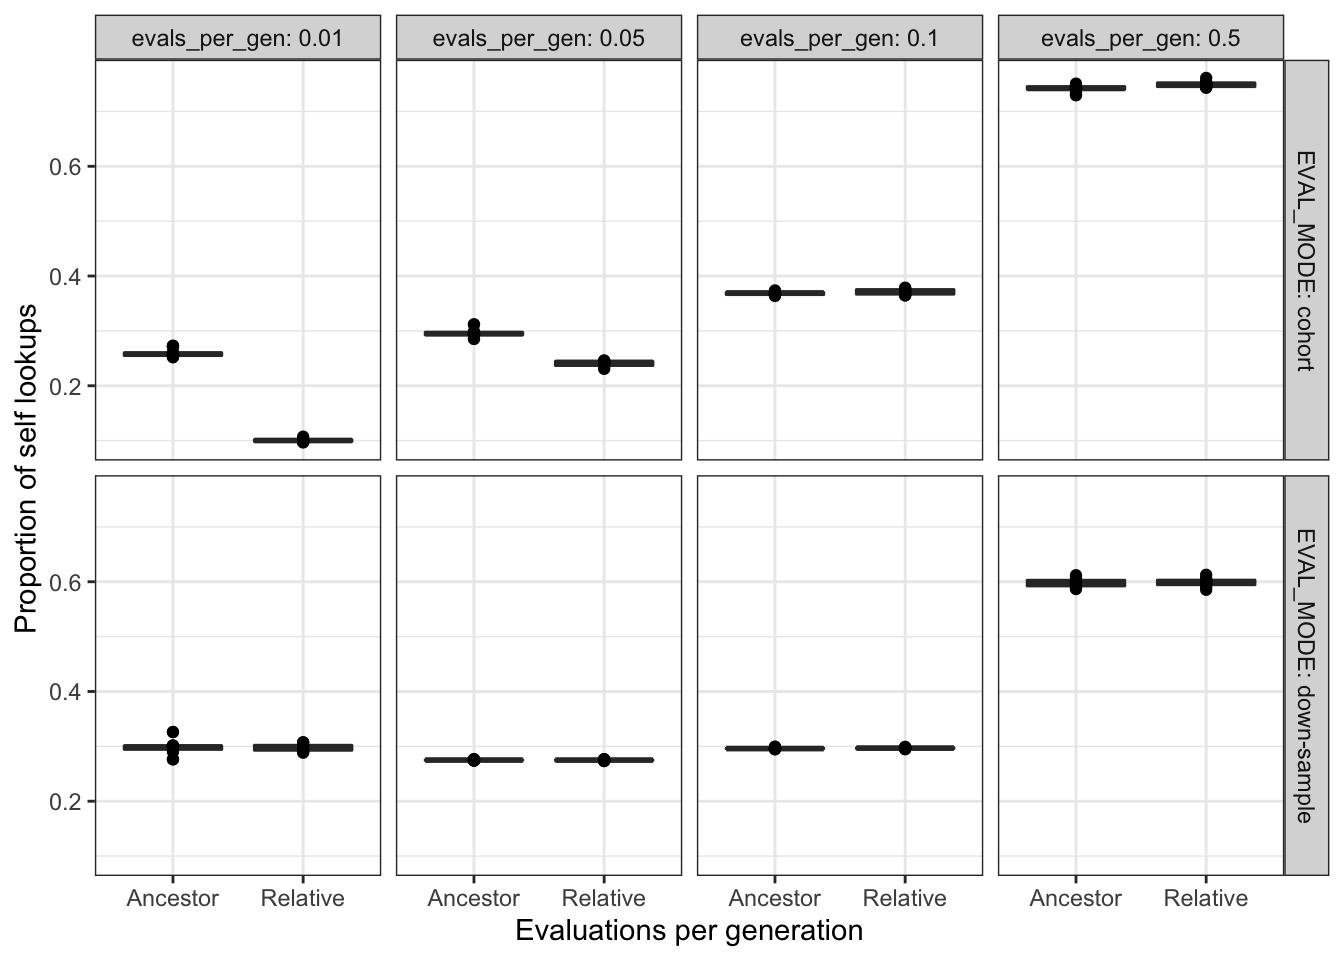
\includegraphics{phylogeny-informed-estimation-supplemental_files/figure-latex/unnamed-chunk-27-1.pdf}

\begin{Shaded}
\begin{Highlighting}[]
\FunctionTok{ggsave}\NormalTok{(}
   \AttributeTok{filename=}\FunctionTok{paste0}\NormalTok{(plot\_directory, }\StringTok{"explore{-}self{-}lookups.pdf"}\NormalTok{)}
\NormalTok{)}
\end{Highlighting}
\end{Shaded}

\begin{verbatim}
## Saving 6.5 x 4.5 in image
\end{verbatim}

\begin{Shaded}
\begin{Highlighting}[]
\NormalTok{est\_source\_data }\SpecialCharTok{\%\textgreater{}\%}
  \FunctionTok{filter}\NormalTok{(DIAGNOSTIC }\SpecialCharTok{==} \StringTok{"multipath{-}exploration"}\NormalTok{) }\SpecialCharTok{\%\textgreater{}\%}
  \FunctionTok{filter}\NormalTok{(EVAL\_MODE }\SpecialCharTok{!=} \StringTok{"full"} \SpecialCharTok{\&}\NormalTok{ EVAL\_FIT\_EST\_MODE }\SpecialCharTok{!=} \StringTok{"None"}\NormalTok{) }\SpecialCharTok{\%\textgreater{}\%}
  \FunctionTok{ggplot}\NormalTok{(}
      \FunctionTok{aes}\NormalTok{(}
        \AttributeTok{x =}\NormalTok{ EVAL\_FIT\_EST\_MODE,}
        \AttributeTok{y =}\NormalTok{ prop\_ancestor\_lookups}
\NormalTok{      )}
\NormalTok{    ) }\SpecialCharTok{+}
    \FunctionTok{geom\_boxplot}\NormalTok{() }\SpecialCharTok{+}
    \FunctionTok{geom\_point}\NormalTok{() }\SpecialCharTok{+}
    \FunctionTok{facet\_grid}\NormalTok{(}
      \AttributeTok{cols =} \FunctionTok{vars}\NormalTok{(evals\_per\_gen),}
      \AttributeTok{rows =} \FunctionTok{vars}\NormalTok{(EVAL\_MODE),}
      \AttributeTok{labeller =}\NormalTok{ label\_both}
\NormalTok{    ) }\SpecialCharTok{+}
    \FunctionTok{scale\_y\_continuous}\NormalTok{(}\StringTok{"Proportion of ancestor lookups"}\NormalTok{) }\SpecialCharTok{+}
    \FunctionTok{scale\_x\_discrete}\NormalTok{(}\StringTok{"Evaluations per generation"}\NormalTok{) }\SpecialCharTok{+}
    \FunctionTok{theme\_bw}\NormalTok{() }\SpecialCharTok{+}
    \FunctionTok{theme}\NormalTok{(}\AttributeTok{legend.position =} \StringTok{"none"}\NormalTok{)}
\end{Highlighting}
\end{Shaded}

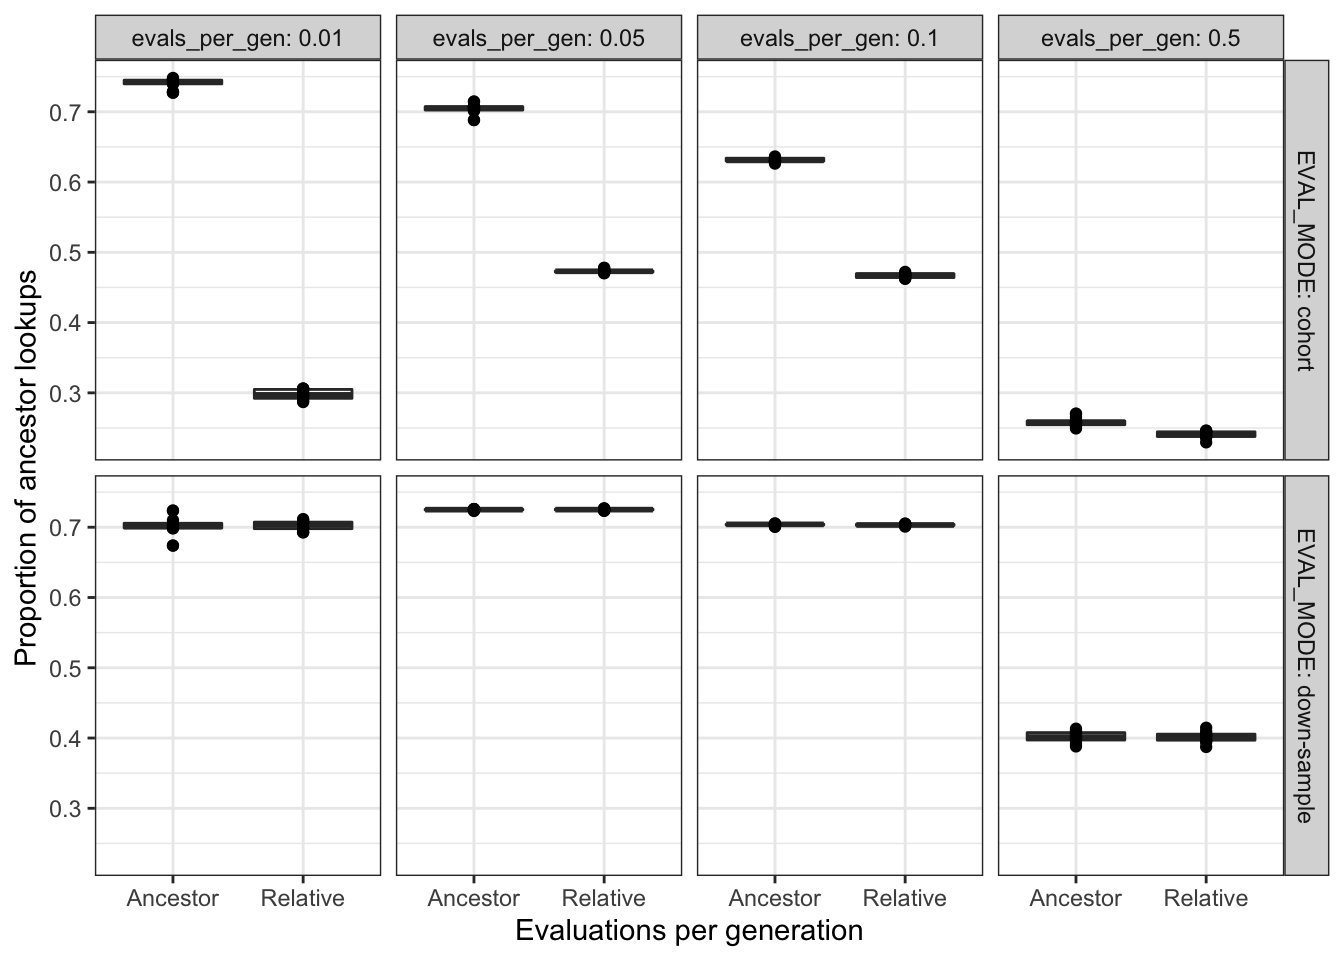
\includegraphics{phylogeny-informed-estimation-supplemental_files/figure-latex/unnamed-chunk-28-1.pdf}

\begin{Shaded}
\begin{Highlighting}[]
\FunctionTok{ggsave}\NormalTok{(}
   \AttributeTok{filename=}\FunctionTok{paste0}\NormalTok{(plot\_directory, }\StringTok{"explore{-}ancestor{-}lookups.pdf"}\NormalTok{)}
\NormalTok{)}
\end{Highlighting}
\end{Shaded}

\begin{verbatim}
## Saving 6.5 x 4.5 in image
\end{verbatim}

\begin{Shaded}
\begin{Highlighting}[]
\NormalTok{est\_source\_data }\SpecialCharTok{\%\textgreater{}\%}
  \FunctionTok{filter}\NormalTok{(DIAGNOSTIC }\SpecialCharTok{==} \StringTok{"multipath{-}exploration"}\NormalTok{) }\SpecialCharTok{\%\textgreater{}\%}
  \FunctionTok{filter}\NormalTok{(EVAL\_MODE }\SpecialCharTok{!=} \StringTok{"full"} \SpecialCharTok{\&}\NormalTok{ EVAL\_FIT\_EST\_MODE }\SpecialCharTok{!=} \StringTok{"None"}\NormalTok{) }\SpecialCharTok{\%\textgreater{}\%}
  \FunctionTok{ggplot}\NormalTok{(}
      \FunctionTok{aes}\NormalTok{(}
        \AttributeTok{x =}\NormalTok{ EVAL\_FIT\_EST\_MODE,}
        \AttributeTok{y =}\NormalTok{ prop\_descendant\_lookups}
\NormalTok{      )}
\NormalTok{    ) }\SpecialCharTok{+}
    \FunctionTok{geom\_boxplot}\NormalTok{() }\SpecialCharTok{+}
    \FunctionTok{geom\_point}\NormalTok{() }\SpecialCharTok{+}
    \FunctionTok{facet\_grid}\NormalTok{(}
      \AttributeTok{cols =} \FunctionTok{vars}\NormalTok{(evals\_per\_gen),}
      \AttributeTok{rows =} \FunctionTok{vars}\NormalTok{(EVAL\_MODE),}
      \AttributeTok{labeller =}\NormalTok{ label\_both}
\NormalTok{    ) }\SpecialCharTok{+}
    \FunctionTok{scale\_y\_continuous}\NormalTok{(}\StringTok{"Proportion of descendant lookups"}\NormalTok{) }\SpecialCharTok{+}
    \FunctionTok{scale\_x\_discrete}\NormalTok{(}\StringTok{"Evaluations per generation"}\NormalTok{) }\SpecialCharTok{+}
    \FunctionTok{theme\_bw}\NormalTok{() }\SpecialCharTok{+}
    \FunctionTok{theme}\NormalTok{(}\AttributeTok{legend.position =} \StringTok{"none"}\NormalTok{)}
\end{Highlighting}
\end{Shaded}

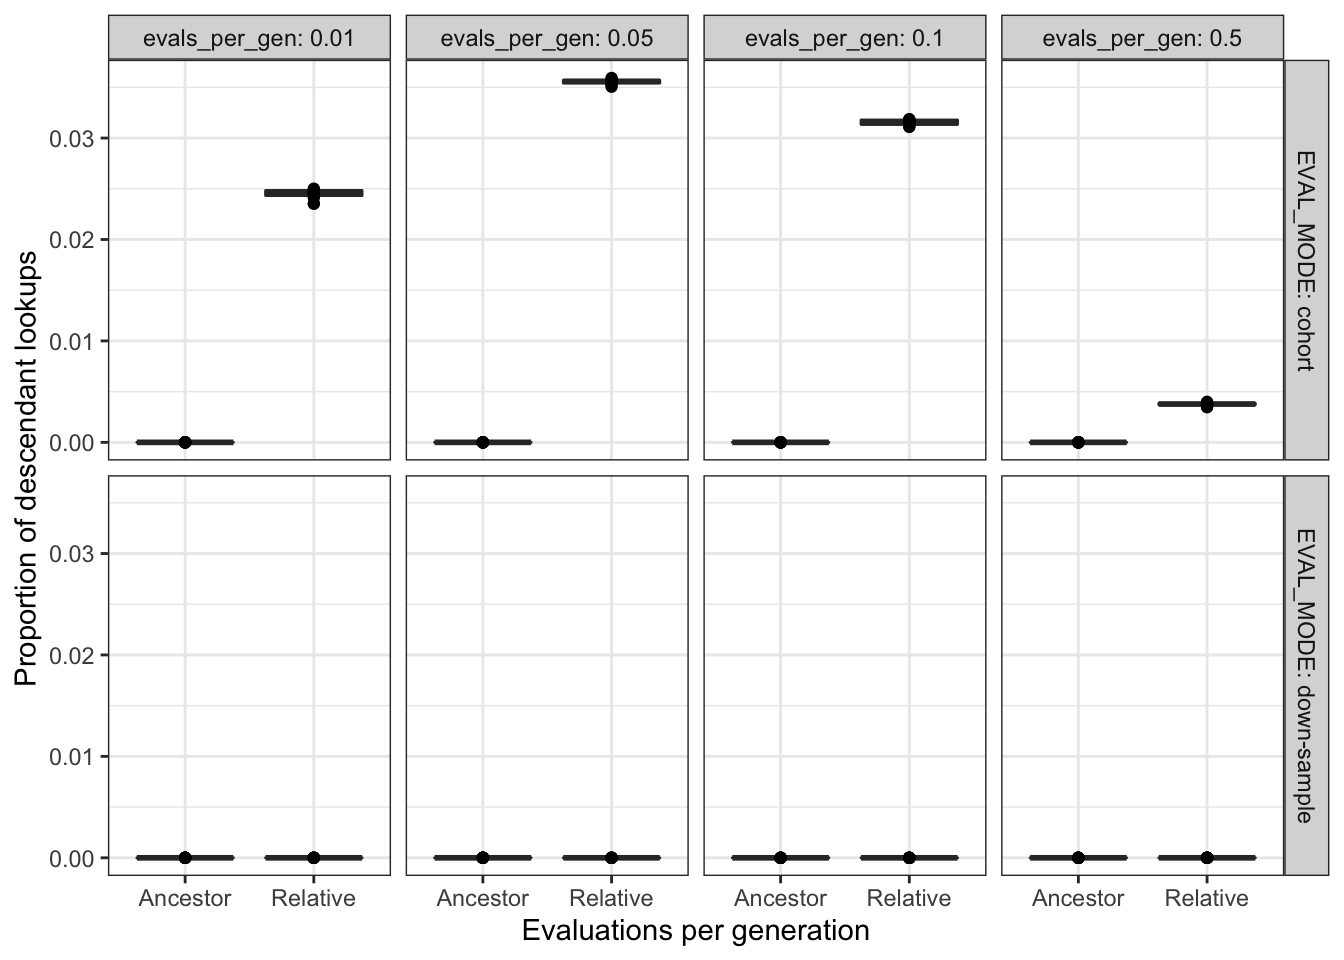
\includegraphics{phylogeny-informed-estimation-supplemental_files/figure-latex/unnamed-chunk-29-1.pdf}

\begin{Shaded}
\begin{Highlighting}[]
\FunctionTok{ggsave}\NormalTok{(}
   \AttributeTok{filename=}\FunctionTok{paste0}\NormalTok{(plot\_directory, }\StringTok{"explore{-}descendant{-}lookups.pdf"}\NormalTok{)}
\NormalTok{)}
\end{Highlighting}
\end{Shaded}

\begin{verbatim}
## Saving 6.5 x 4.5 in image
\end{verbatim}

\begin{Shaded}
\begin{Highlighting}[]
\NormalTok{est\_source\_data }\SpecialCharTok{\%\textgreater{}\%}
  \FunctionTok{filter}\NormalTok{(DIAGNOSTIC }\SpecialCharTok{==} \StringTok{"multipath{-}exploration"}\NormalTok{) }\SpecialCharTok{\%\textgreater{}\%}
  \FunctionTok{filter}\NormalTok{(EVAL\_MODE }\SpecialCharTok{!=} \StringTok{"full"} \SpecialCharTok{\&}\NormalTok{ EVAL\_FIT\_EST\_MODE }\SpecialCharTok{!=} \StringTok{"None"}\NormalTok{) }\SpecialCharTok{\%\textgreater{}\%}
  \FunctionTok{ggplot}\NormalTok{(}
      \FunctionTok{aes}\NormalTok{(}
        \AttributeTok{x =}\NormalTok{ EVAL\_FIT\_EST\_MODE,}
        \AttributeTok{y =}\NormalTok{ prop\_other\_lookups}
\NormalTok{      )}
\NormalTok{    ) }\SpecialCharTok{+}
    \FunctionTok{geom\_boxplot}\NormalTok{() }\SpecialCharTok{+}
    \FunctionTok{geom\_point}\NormalTok{() }\SpecialCharTok{+}
    \FunctionTok{facet\_grid}\NormalTok{(}
      \AttributeTok{cols =} \FunctionTok{vars}\NormalTok{(evals\_per\_gen),}
      \AttributeTok{rows =} \FunctionTok{vars}\NormalTok{(EVAL\_MODE),}
      \AttributeTok{labeller =}\NormalTok{ label\_both}
\NormalTok{    ) }\SpecialCharTok{+}
    \FunctionTok{scale\_y\_continuous}\NormalTok{(}\StringTok{"Proportion of other lookups"}\NormalTok{) }\SpecialCharTok{+}
    \FunctionTok{scale\_x\_discrete}\NormalTok{(}\StringTok{"Evaluations per generation"}\NormalTok{) }\SpecialCharTok{+}
    \FunctionTok{theme\_bw}\NormalTok{() }\SpecialCharTok{+}
    \FunctionTok{theme}\NormalTok{(}\AttributeTok{legend.position =} \StringTok{"none"}\NormalTok{)}
\end{Highlighting}
\end{Shaded}

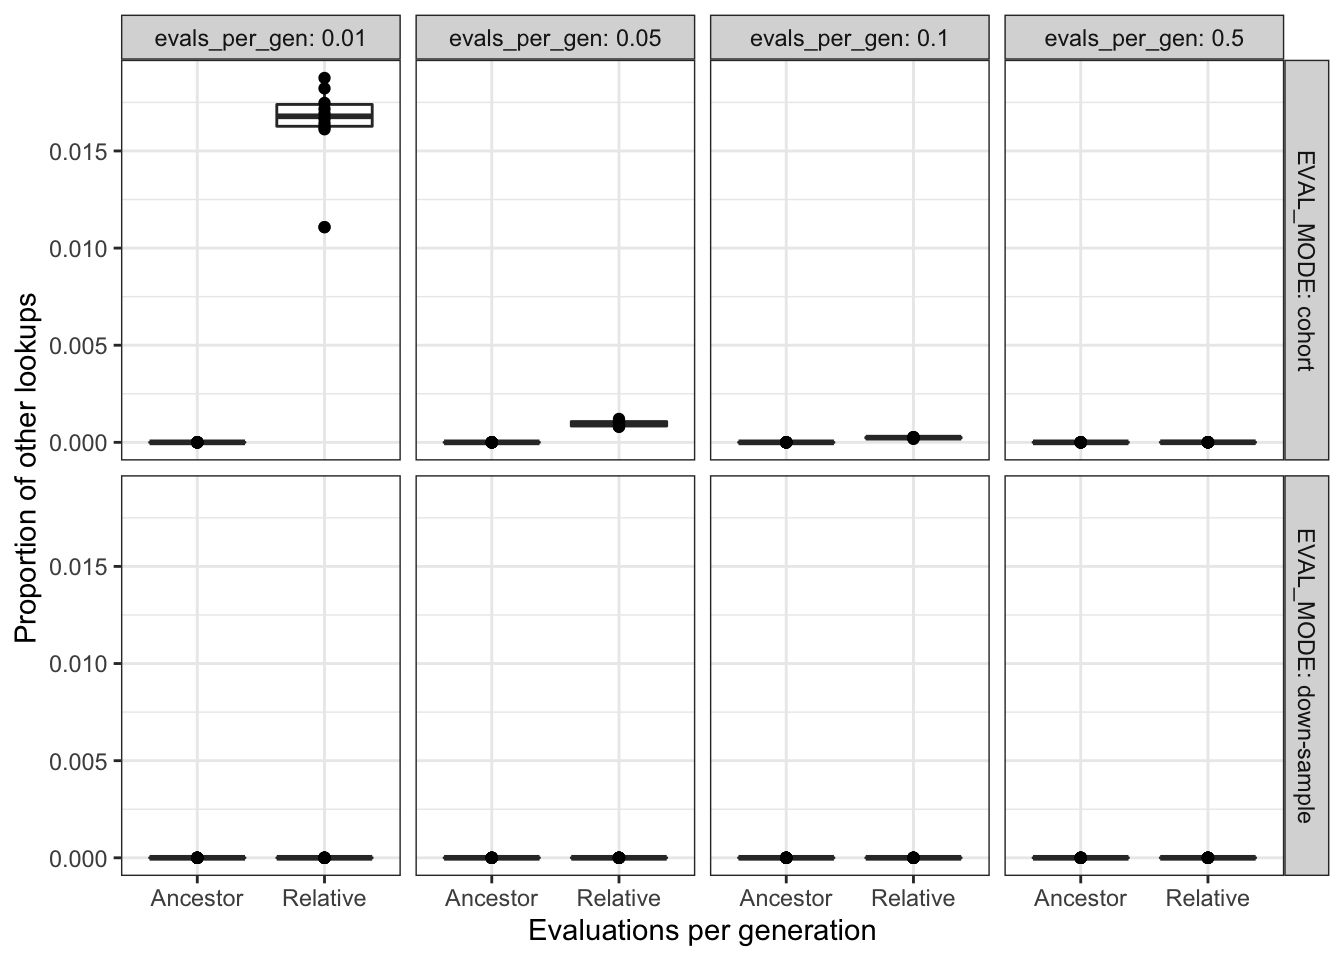
\includegraphics{phylogeny-informed-estimation-supplemental_files/figure-latex/unnamed-chunk-30-1.pdf}

\begin{Shaded}
\begin{Highlighting}[]
\FunctionTok{ggsave}\NormalTok{(}
   \AttributeTok{filename=}\FunctionTok{paste0}\NormalTok{(plot\_directory, }\StringTok{"explore{-}other{-}lookups.pdf"}\NormalTok{)}
\NormalTok{)}
\end{Highlighting}
\end{Shaded}

\begin{verbatim}
## Saving 6.5 x 4.5 in image
\end{verbatim}

\begin{Shaded}
\begin{Highlighting}[]
\NormalTok{est\_source\_data }\SpecialCharTok{\%\textgreater{}\%}
  \FunctionTok{filter}\NormalTok{(DIAGNOSTIC }\SpecialCharTok{==} \StringTok{"multipath{-}exploration"}\NormalTok{) }\SpecialCharTok{\%\textgreater{}\%}
  \FunctionTok{filter}\NormalTok{(EVAL\_MODE }\SpecialCharTok{!=} \StringTok{"full"} \SpecialCharTok{\&}\NormalTok{ EVAL\_FIT\_EST\_MODE }\SpecialCharTok{!=} \StringTok{"None"}\NormalTok{) }\SpecialCharTok{\%\textgreater{}\%}
  \FunctionTok{ggplot}\NormalTok{(}
      \FunctionTok{aes}\NormalTok{(}
        \AttributeTok{x =}\NormalTok{ EVAL\_FIT\_EST\_MODE,}
        \AttributeTok{y =}\NormalTok{ prop\_outside\_lookups}
\NormalTok{      )}
\NormalTok{    ) }\SpecialCharTok{+}
    \FunctionTok{geom\_boxplot}\NormalTok{() }\SpecialCharTok{+}
    \FunctionTok{geom\_point}\NormalTok{() }\SpecialCharTok{+}
    \FunctionTok{facet\_grid}\NormalTok{(}
      \AttributeTok{cols =} \FunctionTok{vars}\NormalTok{(evals\_per\_gen),}
      \AttributeTok{rows =} \FunctionTok{vars}\NormalTok{(EVAL\_MODE),}
      \AttributeTok{labeller =}\NormalTok{ label\_both}
\NormalTok{    ) }\SpecialCharTok{+}
    \FunctionTok{scale\_y\_continuous}\NormalTok{(}\StringTok{"Proportion of outside lookups"}\NormalTok{) }\SpecialCharTok{+}
    \FunctionTok{scale\_x\_discrete}\NormalTok{(}\StringTok{"Evaluations per generation"}\NormalTok{) }\SpecialCharTok{+}
    \FunctionTok{theme\_bw}\NormalTok{() }\SpecialCharTok{+}
    \FunctionTok{theme}\NormalTok{(}\AttributeTok{legend.position =} \StringTok{"none"}\NormalTok{)}
\end{Highlighting}
\end{Shaded}

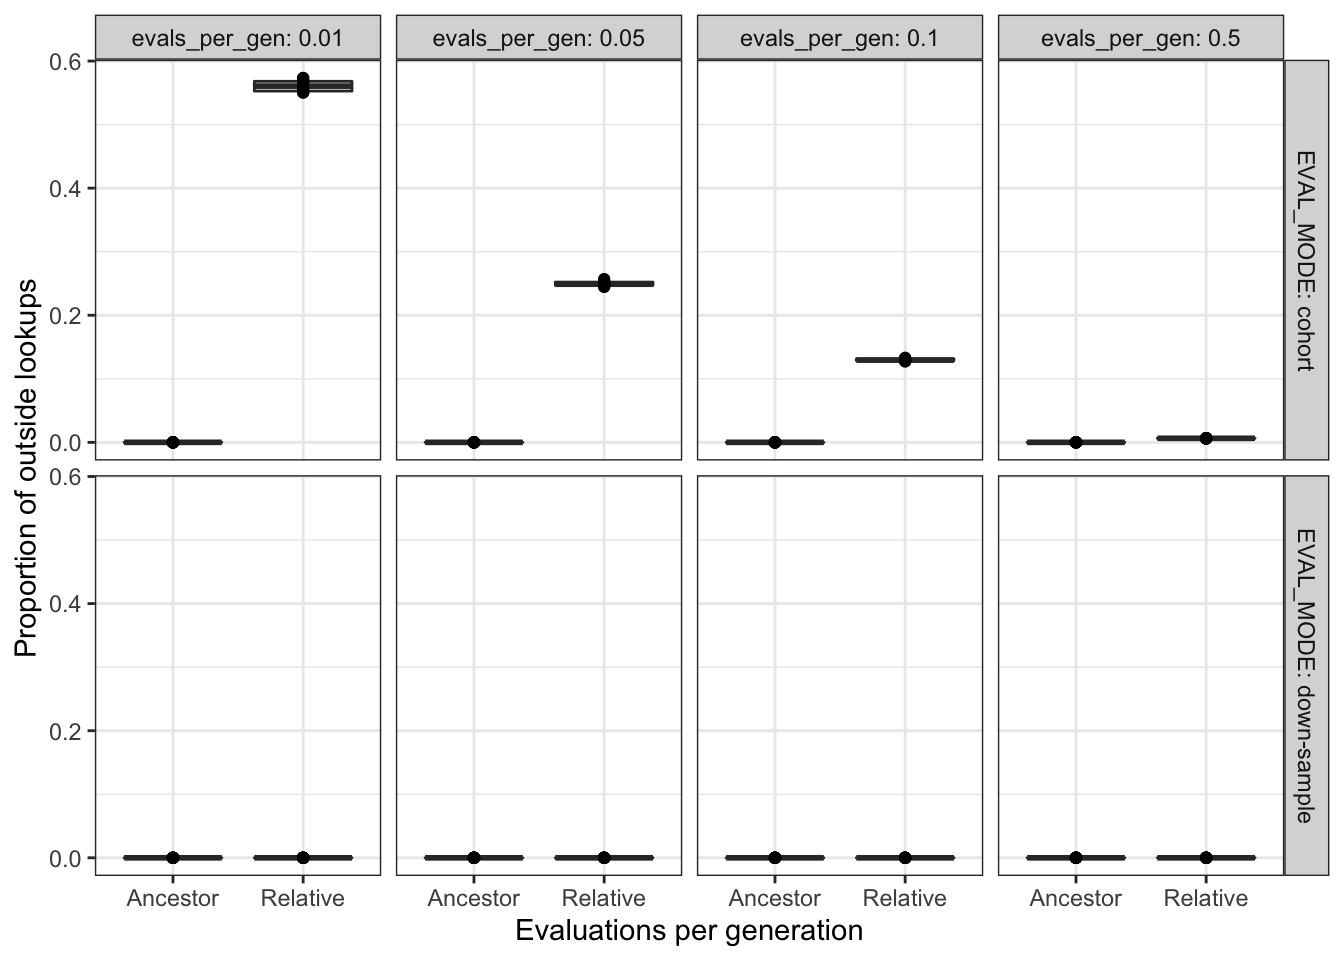
\includegraphics{phylogeny-informed-estimation-supplemental_files/figure-latex/unnamed-chunk-31-1.pdf}

\begin{Shaded}
\begin{Highlighting}[]
\FunctionTok{ggsave}\NormalTok{(}
   \AttributeTok{filename=}\FunctionTok{paste0}\NormalTok{(plot\_directory, }\StringTok{"explore{-}outside{-}lookups.pdf"}\NormalTok{)}
\NormalTok{)}
\end{Highlighting}
\end{Shaded}

\begin{verbatim}
## Saving 6.5 x 4.5 in image
\end{verbatim}

\hypertarget{manuscript-figures}{%
\section{Manuscript figures}\label{manuscript-figures}}

\begin{Shaded}
\begin{Highlighting}[]
\NormalTok{full\_median\_size }\OtherTok{=} \FloatTok{1.5}

\NormalTok{subsample\_labeller }\OtherTok{\textless{}{-}} \ControlFlowTok{function}\NormalTok{(subsample\_level) \{}
  \FunctionTok{return}\NormalTok{(}\FunctionTok{paste}\NormalTok{(}\StringTok{"Subsample level:"}\NormalTok{, subsample\_level))}
\NormalTok{\}}
\end{Highlighting}
\end{Shaded}

\hypertarget{contradictory-objectives}{%
\subsection{Contradictory objectives}\label{contradictory-objectives}}

Build plot panels (1 cohort, 1 down-sample)

\begin{Shaded}
\begin{Highlighting}[]
\NormalTok{build\_con\_obj\_plot }\OtherTok{\textless{}{-}} \ControlFlowTok{function}\NormalTok{(eval\_mode) \{}

\NormalTok{  full\_median }\OtherTok{\textless{}{-}} \FunctionTok{median}\NormalTok{(}
    \FunctionTok{filter}\NormalTok{(}
\NormalTok{      con\_obj\_summary\_data,}
\NormalTok{      eval\_mode\_row }\SpecialCharTok{==}\NormalTok{ eval\_mode }\SpecialCharTok{\&}\NormalTok{ EVAL\_MODE }\SpecialCharTok{==} \StringTok{"full"}
\NormalTok{    )}\SpecialCharTok{$}\NormalTok{pop\_optimal\_trait\_coverage}
\NormalTok{  )}

\NormalTok{  p }\OtherTok{\textless{}{-}}\NormalTok{ con\_obj\_summary\_data }\SpecialCharTok{\%\textgreater{}\%}
    \FunctionTok{filter}\NormalTok{(eval\_mode\_row }\SpecialCharTok{==}\NormalTok{ eval\_mode }\SpecialCharTok{\&}\NormalTok{ EVAL\_MODE }\SpecialCharTok{!=} \StringTok{"full"}\NormalTok{) }\SpecialCharTok{\%\textgreater{}\%}
    \FunctionTok{ggplot}\NormalTok{(}
      \FunctionTok{aes}\NormalTok{(}
        \AttributeTok{x =}\NormalTok{ EVAL\_FIT\_EST\_MODE,}
        \AttributeTok{y =}\NormalTok{ pop\_optimal\_trait\_coverage,}
        \AttributeTok{fill =}\NormalTok{ EVAL\_FIT\_EST\_MODE}
\NormalTok{      )}
\NormalTok{    ) }\SpecialCharTok{+}
    \FunctionTok{geom\_hline}\NormalTok{(}
      \AttributeTok{yintercept =}\NormalTok{ full\_median,}
      \AttributeTok{size =}\NormalTok{ full\_median\_size,}
      \AttributeTok{alpha =} \FloatTok{0.7}\NormalTok{,}
      \AttributeTok{color =} \StringTok{"black"}
\NormalTok{    ) }\SpecialCharTok{+}
    \FunctionTok{geom\_flat\_violin}\NormalTok{(}
      \AttributeTok{position =} \FunctionTok{position\_nudge}\NormalTok{(}\AttributeTok{x =}\NormalTok{ .}\DecValTok{2}\NormalTok{, }\AttributeTok{y =} \DecValTok{0}\NormalTok{),}
      \AttributeTok{alpha =}\NormalTok{ .}\DecValTok{8}\NormalTok{,}
      \AttributeTok{adjust=}\FloatTok{1.5}
\NormalTok{    ) }\SpecialCharTok{+}
    \FunctionTok{geom\_point}\NormalTok{(}
      \AttributeTok{mapping=}\FunctionTok{aes}\NormalTok{(}\AttributeTok{color=}\NormalTok{EVAL\_FIT\_EST\_MODE),}
      \AttributeTok{position =} \FunctionTok{position\_jitter}\NormalTok{(}\AttributeTok{width =}\NormalTok{ .}\DecValTok{15}\NormalTok{),}
      \AttributeTok{size =}\NormalTok{ .}\DecValTok{5}\NormalTok{,}
      \AttributeTok{alpha =} \FloatTok{0.8}
\NormalTok{    ) }\SpecialCharTok{+}
    \FunctionTok{geom\_boxplot}\NormalTok{(}
      \AttributeTok{width =}\NormalTok{ .}\DecValTok{1}\NormalTok{,}
      \AttributeTok{outlier.shape =} \ConstantTok{NA}\NormalTok{,}
      \AttributeTok{alpha =} \FloatTok{0.5}
\NormalTok{    ) }\SpecialCharTok{+}
    \FunctionTok{scale\_y\_continuous}\NormalTok{(}
      \AttributeTok{limits =} \FunctionTok{c}\NormalTok{(}\SpecialCharTok{{-}}\FloatTok{0.5}\NormalTok{, }\DecValTok{50}\NormalTok{)}
\NormalTok{    ) }\SpecialCharTok{+}
    \FunctionTok{scale\_fill\_bright}\NormalTok{() }\SpecialCharTok{+}
    \FunctionTok{scale\_color\_bright}\NormalTok{() }\SpecialCharTok{+}
    \FunctionTok{facet\_wrap}\NormalTok{(}
    \SpecialCharTok{\textasciitilde{}}\NormalTok{ evals\_per\_gen,}
    \AttributeTok{nrow =} \DecValTok{1}\NormalTok{,}
    \AttributeTok{labeller =} \FunctionTok{as\_labeller}\NormalTok{(}
\NormalTok{      subsample\_labeller}
\NormalTok{    )}
\NormalTok{    ) }\SpecialCharTok{+}
    \FunctionTok{labs}\NormalTok{(}
      \AttributeTok{x =} \StringTok{"Estimation mode"}\NormalTok{,}
      \AttributeTok{y =} \StringTok{"Satisfactory trait coverage"}
\NormalTok{    ) }\SpecialCharTok{+}
    \FunctionTok{theme}\NormalTok{(}
      \AttributeTok{legend.position =} \StringTok{"none"}\NormalTok{,}
      \AttributeTok{axis.text.x =} \FunctionTok{element\_text}\NormalTok{(}
        \AttributeTok{angle =} \DecValTok{30}\NormalTok{,}
        \AttributeTok{hjust =} \DecValTok{1}
\NormalTok{      ),}
      \AttributeTok{panel.border =} \FunctionTok{element\_rect}\NormalTok{(}\AttributeTok{color=}\StringTok{"gray"}\NormalTok{, }\AttributeTok{size=}\DecValTok{2}\NormalTok{)}
\NormalTok{    )}

  \FunctionTok{return}\NormalTok{(p)}
\NormalTok{\}}

\NormalTok{con\_obj\_ds\_plot }\OtherTok{\textless{}{-}} \FunctionTok{build\_con\_obj\_plot}\NormalTok{(}\StringTok{"down{-}sample"}\NormalTok{)}
\NormalTok{con\_obj\_cohort\_plot }\OtherTok{\textless{}{-}} \FunctionTok{build\_con\_obj\_plot}\NormalTok{(}\StringTok{"cohort"}\NormalTok{)}
\end{Highlighting}
\end{Shaded}

Combine panels into single plot.

\begin{Shaded}
\begin{Highlighting}[]
\CommentTok{\# Joint title: https://wilkelab.org/cowplot/articles/plot\_grid.html}
\NormalTok{con\_obj\_title }\OtherTok{\textless{}{-}} \FunctionTok{ggdraw}\NormalTok{() }\SpecialCharTok{+}
  \FunctionTok{draw\_label}\NormalTok{(}
    \StringTok{"Contradictory objectives diagnostic"}\NormalTok{,}
    \AttributeTok{fontface =} \StringTok{\textquotesingle{}bold\textquotesingle{}}\NormalTok{,}
    \AttributeTok{x =} \DecValTok{0}\NormalTok{,}
    \AttributeTok{hjust =} \DecValTok{0}
\NormalTok{  ) }\SpecialCharTok{+}
  \FunctionTok{theme}\NormalTok{(}
    \CommentTok{\# add margin on the left of the drawing canvas,}
    \CommentTok{\# so title is aligned with left edge of first plot}
    \AttributeTok{plot.margin =} \FunctionTok{margin}\NormalTok{(}\DecValTok{0}\NormalTok{, }\DecValTok{0}\NormalTok{, }\DecValTok{0}\NormalTok{, }\DecValTok{7}\NormalTok{)}
\NormalTok{  )}

\NormalTok{con\_obj\_grid }\OtherTok{\textless{}{-}} \FunctionTok{plot\_grid}\NormalTok{(}
\NormalTok{  con\_obj\_title,}
\NormalTok{  con\_obj\_ds\_plot }\SpecialCharTok{+}
    \FunctionTok{labs}\NormalTok{(}
      \AttributeTok{title =} \StringTok{"Down{-}sampled lexicase"}
\NormalTok{    ) }\SpecialCharTok{+}
    \FunctionTok{theme}\NormalTok{(}\AttributeTok{axis.title.x =} \FunctionTok{element\_blank}\NormalTok{()),}
\NormalTok{  con\_obj\_cohort\_plot }\SpecialCharTok{+}
    \FunctionTok{labs}\NormalTok{(}
      \AttributeTok{title =} \StringTok{"Cohort lexicase"}
\NormalTok{    ),}
  \AttributeTok{nrow =} \DecValTok{3}\NormalTok{,}
  \AttributeTok{ncol =} \DecValTok{1}\NormalTok{,}
  \CommentTok{\# align = "h",}
  \AttributeTok{labels =} \FunctionTok{c}\NormalTok{(}\StringTok{""}\NormalTok{, }\StringTok{"a"}\NormalTok{, }\StringTok{"b"}\NormalTok{),}
  \AttributeTok{rel\_heights =} \FunctionTok{c}\NormalTok{(}\FloatTok{0.075}\NormalTok{, }\DecValTok{1}\NormalTok{, }\DecValTok{1}\NormalTok{)}
\NormalTok{)}
\NormalTok{con\_obj\_grid}
\end{Highlighting}
\end{Shaded}

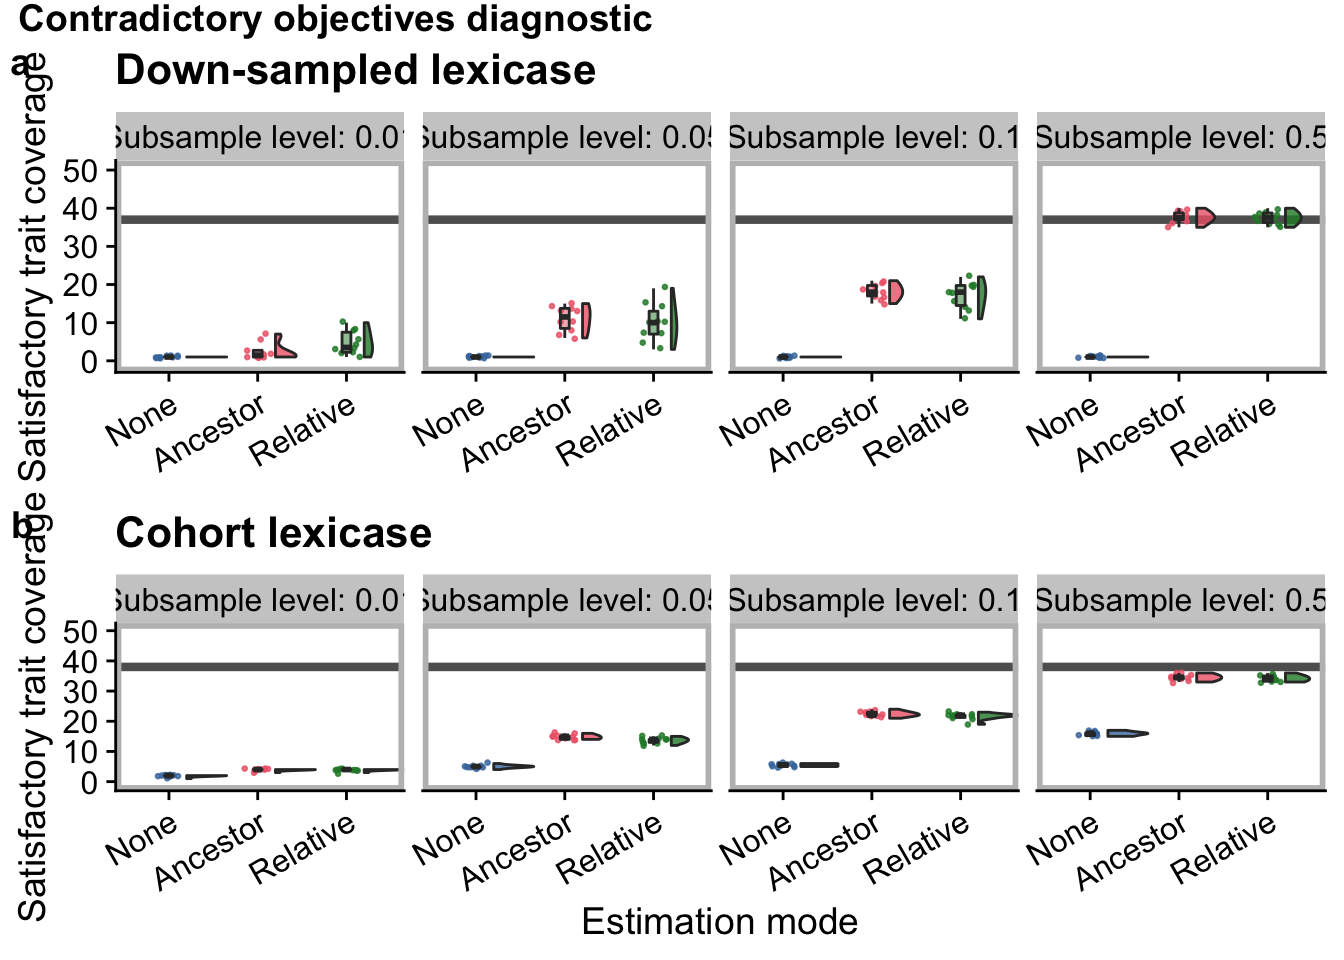
\includegraphics{phylogeny-informed-estimation-supplemental_files/figure-latex/unnamed-chunk-34-1.pdf}

\begin{Shaded}
\begin{Highlighting}[]
\FunctionTok{save\_plot}\NormalTok{(}
  \AttributeTok{filename =} \FunctionTok{paste0}\NormalTok{(plot\_directory, }\StringTok{"2023{-}05{-}10{-}diagnostics{-}con{-}obj{-}final{-}fig.pdf"}\NormalTok{),}
  \AttributeTok{plot =}\NormalTok{ con\_obj\_grid,}
  \AttributeTok{base\_width =} \DecValTok{10}\NormalTok{,}
  \AttributeTok{base\_height =} \DecValTok{8}\NormalTok{,}
  \AttributeTok{dpi =} \DecValTok{600}
\NormalTok{)}
\end{Highlighting}
\end{Shaded}

\hypertarget{multi-path-exploration}{%
\subsection{Multi-path exploration}\label{multi-path-exploration}}

\begin{Shaded}
\begin{Highlighting}[]
\NormalTok{build\_explore\_plot }\OtherTok{\textless{}{-}} \ControlFlowTok{function}\NormalTok{(eval\_mode) \{}

\NormalTok{  full\_median }\OtherTok{\textless{}{-}} \FunctionTok{median}\NormalTok{(}
    \FunctionTok{filter}\NormalTok{(}
\NormalTok{      explore\_summary\_data,}
\NormalTok{      eval\_mode\_row }\SpecialCharTok{==}\NormalTok{ eval\_mode }\SpecialCharTok{\&}\NormalTok{ EVAL\_MODE }\SpecialCharTok{==} \StringTok{"full"}
\NormalTok{    )}\SpecialCharTok{$}\NormalTok{max\_agg\_score}
\NormalTok{  )}

\NormalTok{  p }\OtherTok{\textless{}{-}}\NormalTok{ explore\_summary\_data }\SpecialCharTok{\%\textgreater{}\%}
    \FunctionTok{filter}\NormalTok{(eval\_mode\_row }\SpecialCharTok{==}\NormalTok{ eval\_mode }\SpecialCharTok{\&}\NormalTok{ EVAL\_MODE }\SpecialCharTok{!=} \StringTok{"full"}\NormalTok{) }\SpecialCharTok{\%\textgreater{}\%}
    \FunctionTok{ggplot}\NormalTok{(}
      \FunctionTok{aes}\NormalTok{(}
        \AttributeTok{x =}\NormalTok{ EVAL\_FIT\_EST\_MODE,}
        \AttributeTok{y =}\NormalTok{ max\_agg\_score,}
        \AttributeTok{fill =}\NormalTok{ EVAL\_FIT\_EST\_MODE}
\NormalTok{      )}
\NormalTok{    ) }\SpecialCharTok{+}
    \FunctionTok{geom\_hline}\NormalTok{(}
      \AttributeTok{yintercept =}\NormalTok{ full\_median,}
      \AttributeTok{size =}\NormalTok{ full\_median\_size,}
      \AttributeTok{alpha =} \FloatTok{0.7}\NormalTok{,}
      \AttributeTok{color =} \StringTok{"black"}
\NormalTok{    ) }\SpecialCharTok{+}
    \FunctionTok{geom\_flat\_violin}\NormalTok{(}
      \AttributeTok{position =} \FunctionTok{position\_nudge}\NormalTok{(}\AttributeTok{x =}\NormalTok{ .}\DecValTok{2}\NormalTok{, }\AttributeTok{y =} \DecValTok{0}\NormalTok{),}
      \AttributeTok{alpha =}\NormalTok{ .}\DecValTok{8}\NormalTok{,}
      \AttributeTok{adjust=}\FloatTok{1.5}
\NormalTok{    ) }\SpecialCharTok{+}
    \FunctionTok{geom\_point}\NormalTok{(}
      \AttributeTok{mapping=}\FunctionTok{aes}\NormalTok{(}\AttributeTok{color=}\NormalTok{EVAL\_FIT\_EST\_MODE),}
      \AttributeTok{position =} \FunctionTok{position\_jitter}\NormalTok{(}\AttributeTok{width =}\NormalTok{ .}\DecValTok{15}\NormalTok{),}
      \AttributeTok{size =}\NormalTok{ .}\DecValTok{5}\NormalTok{,}
      \AttributeTok{alpha =} \FloatTok{0.8}
\NormalTok{    ) }\SpecialCharTok{+}
    \FunctionTok{geom\_boxplot}\NormalTok{(}
      \AttributeTok{width =}\NormalTok{ .}\DecValTok{1}\NormalTok{,}
      \AttributeTok{outlier.shape =} \ConstantTok{NA}\NormalTok{,}
      \AttributeTok{alpha =} \FloatTok{0.5}
\NormalTok{    ) }\SpecialCharTok{+}
    \FunctionTok{scale\_y\_continuous}\NormalTok{(}
      \AttributeTok{limits =} \FunctionTok{c}\NormalTok{(}\SpecialCharTok{{-}}\FloatTok{0.5}\NormalTok{, }\DecValTok{10005}\NormalTok{)}
\NormalTok{    ) }\SpecialCharTok{+}
    \FunctionTok{scale\_fill\_bright}\NormalTok{() }\SpecialCharTok{+}
    \FunctionTok{scale\_color\_bright}\NormalTok{() }\SpecialCharTok{+}
    \FunctionTok{facet\_wrap}\NormalTok{(}
    \SpecialCharTok{\textasciitilde{}}\NormalTok{ evals\_per\_gen,}
    \AttributeTok{nrow =} \DecValTok{1}\NormalTok{,}
    \AttributeTok{labeller =} \FunctionTok{as\_labeller}\NormalTok{(}
\NormalTok{      subsample\_labeller}
\NormalTok{    )}
\NormalTok{    ) }\SpecialCharTok{+}
    \FunctionTok{labs}\NormalTok{(}
      \AttributeTok{x =} \StringTok{"Estimation mode"}\NormalTok{,}
      \AttributeTok{y =} \StringTok{"Max aggregate score"}
\NormalTok{    ) }\SpecialCharTok{+}
    \FunctionTok{theme}\NormalTok{(}
      \AttributeTok{legend.position =} \StringTok{"none"}\NormalTok{,}
      \AttributeTok{axis.text.x =} \FunctionTok{element\_text}\NormalTok{(}
        \AttributeTok{angle =} \DecValTok{30}\NormalTok{,}
        \AttributeTok{hjust =} \DecValTok{1}
\NormalTok{      ),}
      \AttributeTok{panel.border =} \FunctionTok{element\_rect}\NormalTok{(}\AttributeTok{color=}\StringTok{"gray"}\NormalTok{, }\AttributeTok{size=}\DecValTok{2}\NormalTok{)}
\NormalTok{    )}

  \FunctionTok{return}\NormalTok{(p)}
\NormalTok{\}}

\NormalTok{explore\_ds\_plot }\OtherTok{\textless{}{-}} \FunctionTok{build\_explore\_plot}\NormalTok{(}\StringTok{"down{-}sample"}\NormalTok{)}
\NormalTok{explore\_cohort\_plot }\OtherTok{\textless{}{-}} \FunctionTok{build\_explore\_plot}\NormalTok{(}\StringTok{"cohort"}\NormalTok{)}

\NormalTok{explore\_ds\_plot}
\end{Highlighting}
\end{Shaded}

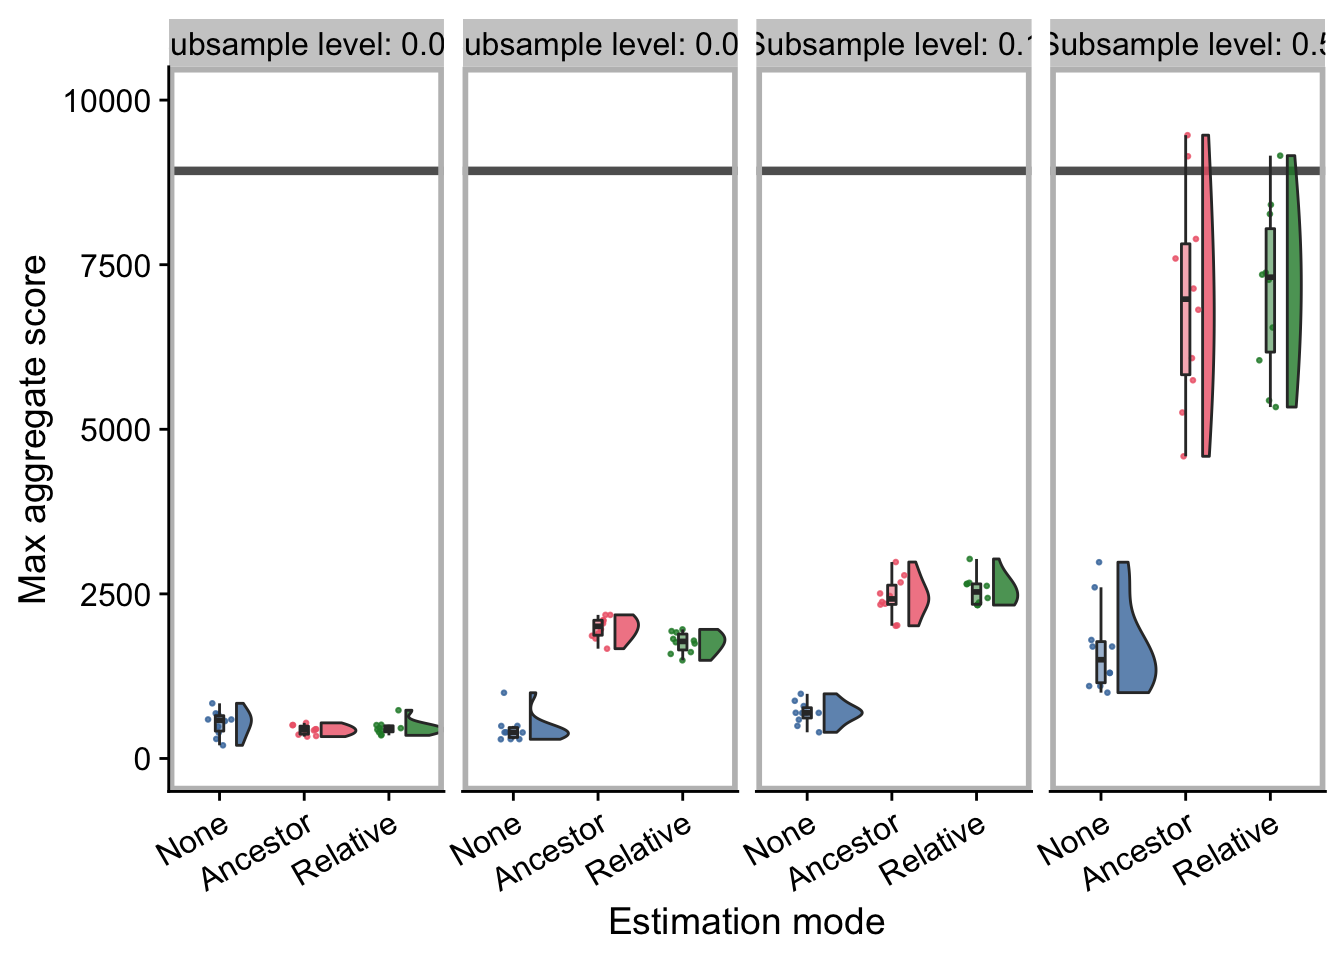
\includegraphics{phylogeny-informed-estimation-supplemental_files/figure-latex/unnamed-chunk-36-1.pdf}

\begin{Shaded}
\begin{Highlighting}[]
\NormalTok{explore\_cohort\_plot}
\end{Highlighting}
\end{Shaded}

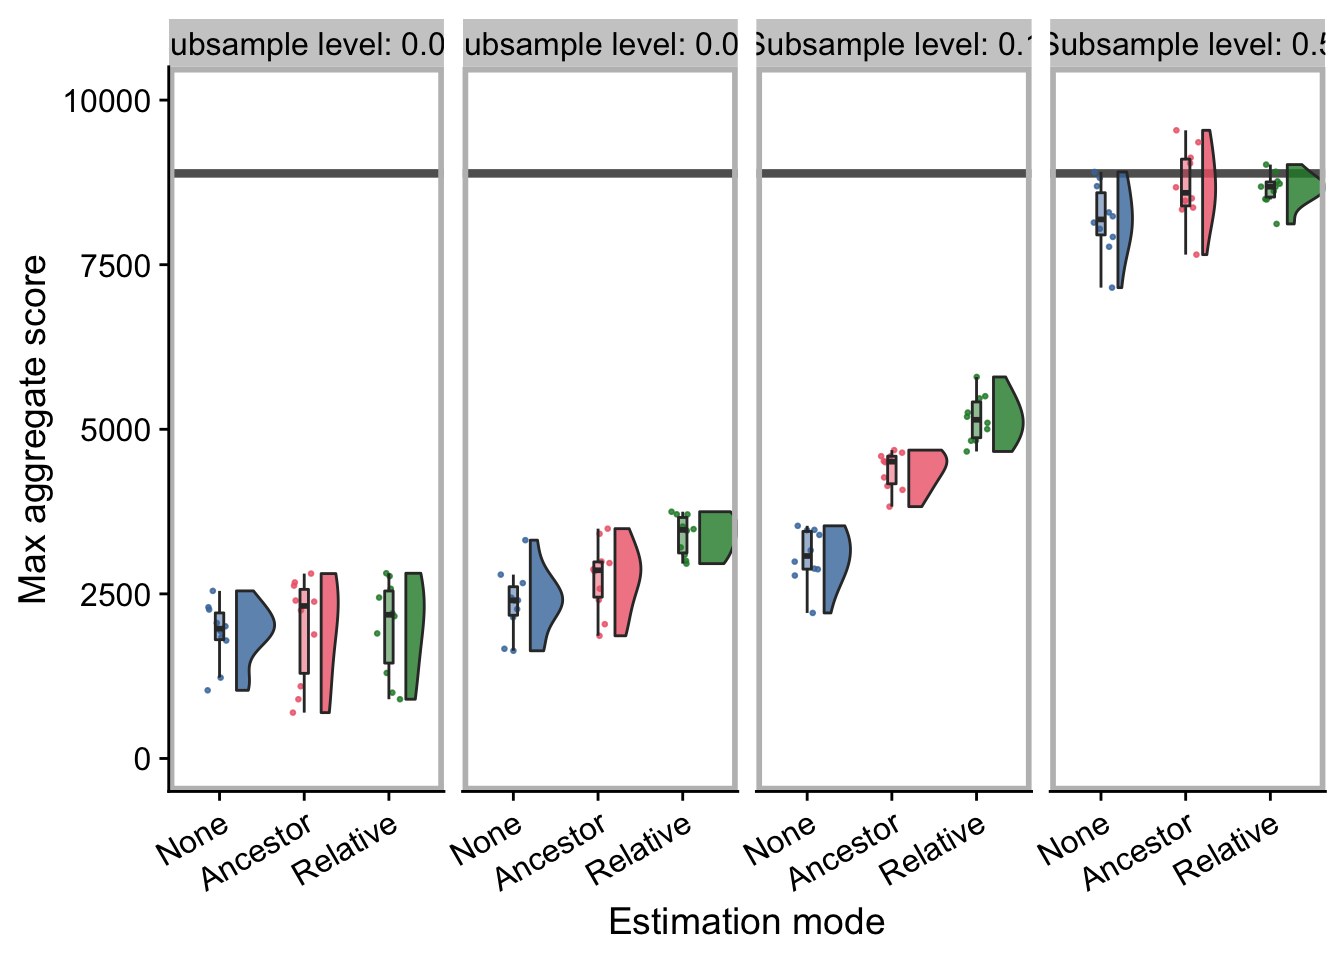
\includegraphics{phylogeny-informed-estimation-supplemental_files/figure-latex/unnamed-chunk-36-2.pdf}

Combine panels into single plot.

\begin{Shaded}
\begin{Highlighting}[]
\CommentTok{\# Joint title: https://wilkelab.org/cowplot/articles/plot\_grid.html}
\NormalTok{explore\_title }\OtherTok{\textless{}{-}} \FunctionTok{ggdraw}\NormalTok{() }\SpecialCharTok{+}
  \FunctionTok{draw\_label}\NormalTok{(}
    \StringTok{"Multi{-}path exploration diagnostic"}\NormalTok{,}
    \AttributeTok{fontface =} \StringTok{\textquotesingle{}bold\textquotesingle{}}\NormalTok{,}
    \AttributeTok{x =} \DecValTok{0}\NormalTok{,}
    \AttributeTok{hjust =} \DecValTok{0}
\NormalTok{  ) }\SpecialCharTok{+}
  \FunctionTok{theme}\NormalTok{(}
    \CommentTok{\# add margin on the left of the drawing canvas,}
    \CommentTok{\# so title is aligned with left edge of first plot}
    \AttributeTok{plot.margin =} \FunctionTok{margin}\NormalTok{(}\DecValTok{0}\NormalTok{, }\DecValTok{0}\NormalTok{, }\DecValTok{0}\NormalTok{, }\DecValTok{7}\NormalTok{)}
\NormalTok{  )}

\NormalTok{explore\_grid }\OtherTok{\textless{}{-}} \FunctionTok{plot\_grid}\NormalTok{(}
\NormalTok{  explore\_title,}
\NormalTok{  explore\_ds\_plot }\SpecialCharTok{+}
    \FunctionTok{labs}\NormalTok{(}
      \AttributeTok{title =} \StringTok{"Down{-}sampled lexicase"}
\NormalTok{    ) }\SpecialCharTok{+}
    \FunctionTok{theme}\NormalTok{(}\AttributeTok{axis.title.x =} \FunctionTok{element\_blank}\NormalTok{()),}
\NormalTok{  explore\_cohort\_plot }\SpecialCharTok{+}
    \FunctionTok{labs}\NormalTok{(}
      \AttributeTok{title =} \StringTok{"Cohort lexicase"}
\NormalTok{    ),}
  \AttributeTok{nrow =} \DecValTok{3}\NormalTok{,}
  \AttributeTok{ncol =} \DecValTok{1}\NormalTok{,}
  \CommentTok{\# align = "h",}
  \AttributeTok{labels =} \FunctionTok{c}\NormalTok{(}\StringTok{""}\NormalTok{, }\StringTok{"a"}\NormalTok{, }\StringTok{"b"}\NormalTok{),}
  \AttributeTok{rel\_heights =} \FunctionTok{c}\NormalTok{(}\FloatTok{0.075}\NormalTok{, }\DecValTok{1}\NormalTok{, }\DecValTok{1}\NormalTok{)}
\NormalTok{)}
\NormalTok{explore\_grid}
\end{Highlighting}
\end{Shaded}

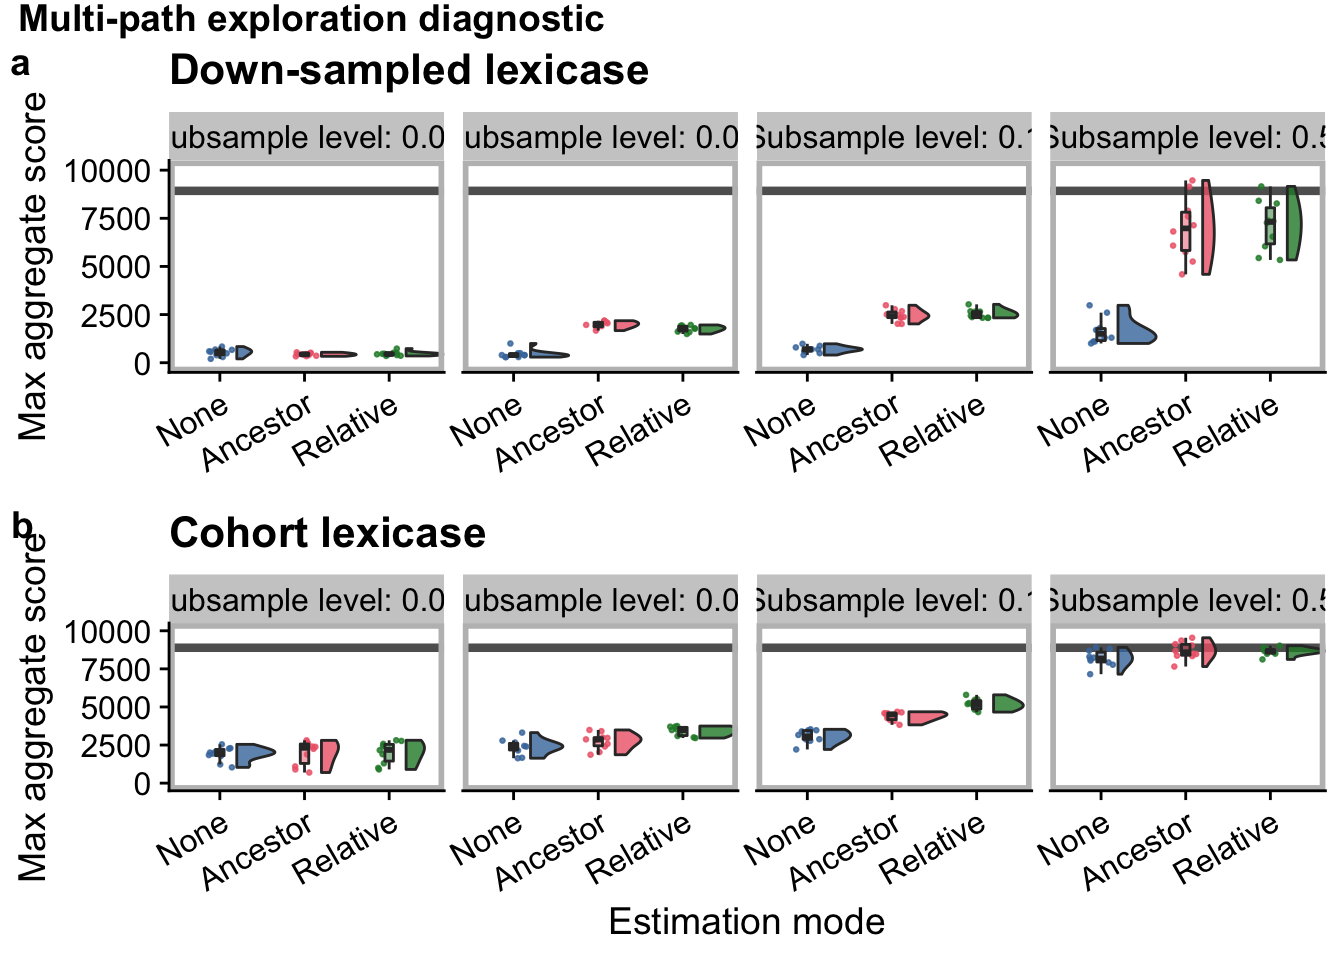
\includegraphics{phylogeny-informed-estimation-supplemental_files/figure-latex/unnamed-chunk-37-1.pdf}

\begin{Shaded}
\begin{Highlighting}[]
\FunctionTok{save\_plot}\NormalTok{(}
  \AttributeTok{filename =} \FunctionTok{paste0}\NormalTok{(plot\_directory, }\StringTok{"2023{-}05{-}10{-}diagnostics{-}explore{-}final{-}fig.pdf"}\NormalTok{),}
  \AttributeTok{plot =}\NormalTok{ explore\_grid,}
  \AttributeTok{base\_width =} \DecValTok{10}\NormalTok{,}
  \AttributeTok{base\_height =} \DecValTok{8}\NormalTok{,}
  \AttributeTok{dpi =} \DecValTok{600}
\NormalTok{)}
\end{Highlighting}
\end{Shaded}

\hypertarget{program-synthesis-experiments}{%
\chapter{Program synthesis experiments}\label{program-synthesis-experiments}}

\begin{Shaded}
\begin{Highlighting}[]
\NormalTok{experiment\_slug }\OtherTok{\textless{}{-}} \StringTok{"2023{-}05{-}08{-}psynth"}

\NormalTok{working\_directory }\OtherTok{\textless{}{-}} \FunctionTok{paste0}\NormalTok{(}
  \StringTok{"experiments/"}\NormalTok{,}
\NormalTok{  experiment\_slug,}
  \StringTok{"/analysis/"}
\NormalTok{)}

\ControlFlowTok{if}\NormalTok{ (}\FunctionTok{exists}\NormalTok{(}\StringTok{"bookdown\_wd\_prefix"}\NormalTok{)) \{}
\NormalTok{  working\_directory }\OtherTok{\textless{}{-}} \FunctionTok{paste0}\NormalTok{(}
\NormalTok{    bookdown\_wd\_prefix,}
\NormalTok{    working\_directory}
\NormalTok{  )}
\NormalTok{\}}
\end{Highlighting}
\end{Shaded}

\hypertarget{dependencies-1}{%
\section{Dependencies}\label{dependencies-1}}

\begin{Shaded}
\begin{Highlighting}[]
\FunctionTok{library}\NormalTok{(tidyverse)}
\FunctionTok{library}\NormalTok{(ggplot2)}
\FunctionTok{library}\NormalTok{(cowplot)}
\FunctionTok{library}\NormalTok{(RColorBrewer)}
\FunctionTok{library}\NormalTok{(khroma)}
\FunctionTok{library}\NormalTok{(rstatix)}
\FunctionTok{library}\NormalTok{(knitr)}
\FunctionTok{source}\NormalTok{(}\StringTok{"https://gist.githubusercontent.com/benmarwick/2a1bb0133ff568cbe28d/raw/fb53bd97121f7f9ce947837ef1a4c65a73bffb3f/geom\_flat\_violin.R"}\NormalTok{)}
\end{Highlighting}
\end{Shaded}

\begin{Shaded}
\begin{Highlighting}[]
\FunctionTok{print}\NormalTok{(version)}
\end{Highlighting}
\end{Shaded}

\begin{verbatim}
##                _                           
## platform       aarch64-apple-darwin20      
## arch           aarch64                     
## os             darwin20                    
## system         aarch64, darwin20           
## status                                     
## major          4                           
## minor          2.1                         
## year           2022                        
## month          06                          
## day            23                          
## svn rev        82513                       
## language       R                           
## version.string R version 4.2.1 (2022-06-23)
## nickname       Funny-Looking Kid
\end{verbatim}

\hypertarget{setup-1}{%
\section{Setup}\label{setup-1}}

\begin{Shaded}
\begin{Highlighting}[]
\CommentTok{\# Configure our default graphing theme}
\FunctionTok{theme\_set}\NormalTok{(}\FunctionTok{theme\_cowplot}\NormalTok{())}
\CommentTok{\# Create a directory to store plots}
\NormalTok{plot\_directory }\OtherTok{\textless{}{-}} \FunctionTok{paste0}\NormalTok{(working\_directory, }\StringTok{"plots/"}\NormalTok{)}
\FunctionTok{dir.create}\NormalTok{(plot\_directory, }\AttributeTok{showWarnings=}\ConstantTok{FALSE}\NormalTok{)}
\end{Highlighting}
\end{Shaded}

\hypertarget{load-summary-data}{%
\subsection{Load summary data}\label{load-summary-data}}

\begin{Shaded}
\begin{Highlighting}[]
\NormalTok{summary\_data\_loc }\OtherTok{\textless{}{-}} \FunctionTok{paste0}\NormalTok{(working\_directory, }\StringTok{"data/aggregate.csv"}\NormalTok{)}
\NormalTok{summary\_data }\OtherTok{\textless{}{-}} \FunctionTok{read\_csv}\NormalTok{(summary\_data\_loc)}
\end{Highlighting}
\end{Shaded}

\begin{verbatim}
## Rows: 3120 Columns: 73
## -- Column specification ----------------------------------------------------------------------------------------------------------------------------------------------------------------------------------
## Delimiter: ","
## chr (11): ANCESTOR_FILE_PATH, EVAL_FIT_EST_MODE, EVAL_MODE, POP_INIT_MODE, P...
## dbl (62): EVAL_CPU_CYCLES_PER_TEST, EVAL_MAX_PHYLO_SEARCH_DEPTH, MAX_ACTIVE_...
## 
## i Use `spec()` to retrieve the full column specification for this data.
## i Specify the column types or set `show_col_types = FALSE` to quiet this message.
\end{verbatim}

\begin{Shaded}
\begin{Highlighting}[]
\NormalTok{summary\_data }\OtherTok{\textless{}{-}}\NormalTok{ summary\_data }\SpecialCharTok{\%\textgreater{}\%}
  \FunctionTok{mutate}\NormalTok{(}
    \AttributeTok{eval\_mode\_row =} \FunctionTok{case\_when}\NormalTok{(}
\NormalTok{      EVAL\_MODE }\SpecialCharTok{==} \StringTok{"full"} \SpecialCharTok{\&}\NormalTok{ TEST\_DOWNSAMPLE\_RATE }\SpecialCharTok{==} \StringTok{"1"} \SpecialCharTok{\textasciitilde{}} \StringTok{"down{-}sample"}\NormalTok{,}
\NormalTok{      EVAL\_MODE }\SpecialCharTok{==} \StringTok{"full"} \SpecialCharTok{\&}\NormalTok{ NUM\_COHORTS }\SpecialCharTok{==} \StringTok{"1"} \SpecialCharTok{\textasciitilde{}} \StringTok{"cohort"}\NormalTok{,}
      \AttributeTok{.default =}\NormalTok{ EVAL\_MODE}
\NormalTok{    ),}
    \AttributeTok{evals\_per\_gen =} \FunctionTok{case\_when}\NormalTok{(}
\NormalTok{      EVAL\_MODE }\SpecialCharTok{==} \StringTok{"cohort"} \SpecialCharTok{\textasciitilde{}} \FloatTok{1.0} \SpecialCharTok{/}\NormalTok{ NUM\_COHORTS,}
\NormalTok{      EVAL\_MODE }\SpecialCharTok{==} \StringTok{"down{-}sample"} \SpecialCharTok{\textasciitilde{}}\NormalTok{ TEST\_DOWNSAMPLE\_RATE,}
\NormalTok{      EVAL\_MODE }\SpecialCharTok{==} \StringTok{"full"} \SpecialCharTok{\textasciitilde{}} \FloatTok{1.0}
\NormalTok{    ),}
    \AttributeTok{EVAL\_FIT\_EST\_MODE =} \FunctionTok{case\_when}\NormalTok{(}
\NormalTok{      EVAL\_FIT\_EST\_MODE }\SpecialCharTok{==} \StringTok{"ancestor{-}opt"} \SpecialCharTok{\textasciitilde{}} \StringTok{"ancestor"}\NormalTok{,}
\NormalTok{      EVAL\_FIT\_EST\_MODE }\SpecialCharTok{==} \StringTok{"relative{-}opt"} \SpecialCharTok{\textasciitilde{}} \StringTok{"relative"}\NormalTok{,}
      \AttributeTok{.default =}\NormalTok{ EVAL\_FIT\_EST\_MODE}
\NormalTok{    ),}
    \AttributeTok{.keep =} \StringTok{"all"}
\NormalTok{  ) }\SpecialCharTok{\%\textgreater{}\%}
  \FunctionTok{mutate}\NormalTok{(}
    \AttributeTok{evals\_per\_gen =} \FunctionTok{as.factor}\NormalTok{(evals\_per\_gen),}
    \AttributeTok{PROBLEM =} \FunctionTok{as.factor}\NormalTok{(PROBLEM),}
    \AttributeTok{SELECTION =} \FunctionTok{as.factor}\NormalTok{(SELECTION),}
    \AttributeTok{EVAL\_MODE =} \FunctionTok{as.factor}\NormalTok{(EVAL\_MODE),}
    \AttributeTok{NUM\_COHORTS =} \FunctionTok{as.factor}\NormalTok{(NUM\_COHORTS),}
    \AttributeTok{TEST\_DOWNSAMPLE\_RATE =} \FunctionTok{as.factor}\NormalTok{(TEST\_DOWNSAMPLE\_RATE),}
    \AttributeTok{EVAL\_FIT\_EST\_MODE =} \FunctionTok{factor}\NormalTok{(}
\NormalTok{      EVAL\_FIT\_EST\_MODE,}
      \AttributeTok{levels =} \FunctionTok{c}\NormalTok{(}
        \StringTok{"none"}\NormalTok{,}
        \StringTok{"ancestor"}\NormalTok{,}
        \StringTok{"relative"}
\NormalTok{      ),}
      \AttributeTok{labels =} \FunctionTok{c}\NormalTok{(}
        \StringTok{"None"}\NormalTok{,}
        \StringTok{"Ancestor"}\NormalTok{,}
        \StringTok{"Relative"}
\NormalTok{      )}
\NormalTok{    ),}
    \AttributeTok{.keep =} \StringTok{"all"}
\NormalTok{  )}

\NormalTok{solution\_counts }\OtherTok{\textless{}{-}}\NormalTok{ summary\_data }\SpecialCharTok{\%\textgreater{}\%}
  \FunctionTok{group\_by}\NormalTok{(}
\NormalTok{    PROBLEM,}
\NormalTok{    evals\_per\_gen,}
\NormalTok{    eval\_mode\_row,}
\NormalTok{    EVAL\_FIT\_EST\_MODE,}
\NormalTok{    EVAL\_MODE}
\NormalTok{  ) }\SpecialCharTok{\%\textgreater{}\%}
  \FunctionTok{summarize}\NormalTok{(}
    \AttributeTok{solution\_count =} \FunctionTok{sum}\NormalTok{(found\_solution }\SpecialCharTok{==} \StringTok{"1"}\NormalTok{),}
    \AttributeTok{replicates =} \FunctionTok{n}\NormalTok{(),}
    \AttributeTok{no\_solution\_count =} \FunctionTok{n}\NormalTok{() }\SpecialCharTok{{-}} \FunctionTok{sum}\NormalTok{(found\_solution }\SpecialCharTok{==} \StringTok{"1"}\NormalTok{)}
\NormalTok{  )}
\end{Highlighting}
\end{Shaded}

\begin{verbatim}
## `summarise()` has grouped output by 'PROBLEM', 'evals_per_gen', 'eval_mode_row',
## 'EVAL_FIT_EST_MODE'. You can override using the `.groups` argument.
\end{verbatim}

\begin{Shaded}
\begin{Highlighting}[]
\FunctionTok{print}\NormalTok{(solution\_counts, }\AttributeTok{n=}\DecValTok{140}\NormalTok{)}
\end{Highlighting}
\end{Shaded}

\begin{verbatim}
## # A tibble: 104 x 8
## # Groups:   PROBLEM, evals_per_gen, eval_mode_row, EVAL_FIT_EST_MODE [104]
##     PROBLEM        evals_per_gen eval_~1 EVAL_~2 EVAL_~3 solut~4 repli~5 no_so~6
##     <fct>          <fct>         <chr>   <fct>   <fct>     <int>   <int>   <int>
##   1 fizz-buzz      0.01          cohort  None    cohort        0      30      30
##   2 fizz-buzz      0.01          cohort  Ancest~ cohort        2      30      28
##   3 fizz-buzz      0.01          cohort  Relati~ cohort        3      30      27
##   4 fizz-buzz      0.01          down-s~ None    down-s~       0      30      30
##   5 fizz-buzz      0.01          down-s~ Ancest~ down-s~       0      30      30
##   6 fizz-buzz      0.01          down-s~ Relati~ down-s~       0      30      30
##   7 fizz-buzz      0.05          cohort  None    cohort        5      30      25
##   8 fizz-buzz      0.05          cohort  Ancest~ cohort        3      30      27
##   9 fizz-buzz      0.05          cohort  Relati~ cohort        7      30      23
##  10 fizz-buzz      0.05          down-s~ None    down-s~      20      30      10
##  11 fizz-buzz      0.05          down-s~ Ancest~ down-s~       2      30      28
##  12 fizz-buzz      0.05          down-s~ Relati~ down-s~       2      30      28
##  13 fizz-buzz      0.1           cohort  None    cohort        1      30      29
##  14 fizz-buzz      0.1           cohort  Ancest~ cohort        3      30      27
##  15 fizz-buzz      0.1           cohort  Relati~ cohort        9      30      21
##  16 fizz-buzz      0.1           down-s~ None    down-s~       8      30      22
##  17 fizz-buzz      0.1           down-s~ Ancest~ down-s~       8      30      22
##  18 fizz-buzz      0.1           down-s~ Relati~ down-s~       7      30      23
##  19 fizz-buzz      0.5           cohort  None    cohort        0      30      30
##  20 fizz-buzz      0.5           cohort  Ancest~ cohort        9      30      21
##  21 fizz-buzz      0.5           cohort  Relati~ cohort        6      30      24
##  22 fizz-buzz      0.5           down-s~ None    down-s~       0      30      30
##  23 fizz-buzz      0.5           down-s~ Ancest~ down-s~       7      30      23
##  24 fizz-buzz      0.5           down-s~ Relati~ down-s~       7      30      23
##  25 fizz-buzz      1             cohort  None    full          0      30      30
##  26 fizz-buzz      1             down-s~ None    full          0      30      30
##  27 grade          0.01          cohort  None    cohort       20      30      10
##  28 grade          0.01          cohort  Ancest~ cohort       18      30      12
##  29 grade          0.01          cohort  Relati~ cohort       23      30       7
##  30 grade          0.01          down-s~ None    down-s~       1      30      29
##  31 grade          0.01          down-s~ Ancest~ down-s~      10      30      20
##  32 grade          0.01          down-s~ Relati~ down-s~      11      30      19
##  33 grade          0.05          cohort  None    cohort       18      30      12
##  34 grade          0.05          cohort  Ancest~ cohort       13      30      17
##  35 grade          0.05          cohort  Relati~ cohort       19      30      11
##  36 grade          0.05          down-s~ None    down-s~      22      30       8
##  37 grade          0.05          down-s~ Ancest~ down-s~      12      30      18
##  38 grade          0.05          down-s~ Relati~ down-s~      11      30      19
##  39 grade          0.1           cohort  None    cohort       12      30      18
##  40 grade          0.1           cohort  Ancest~ cohort       20      30      10
##  41 grade          0.1           cohort  Relati~ cohort       15      30      15
##  42 grade          0.1           down-s~ None    down-s~      22      30       8
##  43 grade          0.1           down-s~ Ancest~ down-s~      13      30      17
##  44 grade          0.1           down-s~ Relati~ down-s~      11      30      19
##  45 grade          0.5           cohort  None    cohort        4      30      26
##  46 grade          0.5           cohort  Ancest~ cohort        2      30      28
##  47 grade          0.5           cohort  Relati~ cohort        4      30      26
##  48 grade          0.5           down-s~ None    down-s~       5      30      25
##  49 grade          0.5           down-s~ Ancest~ down-s~       9      30      21
##  50 grade          0.5           down-s~ Relati~ down-s~       4      30      26
##  51 grade          1             cohort  None    full          1      30      29
##  52 grade          1             down-s~ None    full          1      30      29
##  53 median         0.01          cohort  None    cohort        0      30      30
##  54 median         0.01          cohort  Ancest~ cohort       22      30       8
##  55 median         0.01          cohort  Relati~ cohort       27      30       3
##  56 median         0.01          down-s~ None    down-s~       8      30      22
##  57 median         0.01          down-s~ Ancest~ down-s~      13      30      17
##  58 median         0.01          down-s~ Relati~ down-s~      14      30      16
##  59 median         0.05          cohort  None    cohort       12      30      18
##  60 median         0.05          cohort  Ancest~ cohort       23      30       7
##  61 median         0.05          cohort  Relati~ cohort       25      30       5
##  62 median         0.05          down-s~ None    down-s~       4      30      26
##  63 median         0.05          down-s~ Ancest~ down-s~      19      30      11
##  64 median         0.05          down-s~ Relati~ down-s~      23      30       7
##  65 median         0.1           cohort  None    cohort       15      30      15
##  66 median         0.1           cohort  Ancest~ cohort       26      30       4
##  67 median         0.1           cohort  Relati~ cohort       24      30       6
##  68 median         0.1           down-s~ None    down-s~      16      30      14
##  69 median         0.1           down-s~ Ancest~ down-s~      21      30       9
##  70 median         0.1           down-s~ Relati~ down-s~      22      30       8
##  71 median         0.5           cohort  None    cohort        5      30      25
##  72 median         0.5           cohort  Ancest~ cohort       12      30      18
##  73 median         0.5           cohort  Relati~ cohort       13      30      17
##  74 median         0.5           down-s~ None    down-s~       2      30      28
##  75 median         0.5           down-s~ Ancest~ down-s~      15      30      15
##  76 median         0.5           down-s~ Relati~ down-s~      13      30      17
##  77 median         1             cohort  None    full          1      30      29
##  78 median         1             down-s~ None    full          1      30      29
##  79 small-or-large 0.01          cohort  None    cohort        0      30      30
##  80 small-or-large 0.01          cohort  Ancest~ cohort        1      30      29
##  81 small-or-large 0.01          cohort  Relati~ cohort        0      30      30
##  82 small-or-large 0.01          down-s~ None    down-s~       0      30      30
##  83 small-or-large 0.01          down-s~ Ancest~ down-s~       0      30      30
##  84 small-or-large 0.01          down-s~ Relati~ down-s~       0      30      30
##  85 small-or-large 0.05          cohort  None    cohort        0      30      30
##  86 small-or-large 0.05          cohort  Ancest~ cohort        0      30      30
##  87 small-or-large 0.05          cohort  Relati~ cohort        1      30      29
##  88 small-or-large 0.05          down-s~ None    down-s~       0      30      30
##  89 small-or-large 0.05          down-s~ Ancest~ down-s~       0      30      30
##  90 small-or-large 0.05          down-s~ Relati~ down-s~       0      30      30
##  91 small-or-large 0.1           cohort  None    cohort        0      30      30
##  92 small-or-large 0.1           cohort  Ancest~ cohort        0      30      30
##  93 small-or-large 0.1           cohort  Relati~ cohort        0      30      30
##  94 small-or-large 0.1           down-s~ None    down-s~       0      30      30
##  95 small-or-large 0.1           down-s~ Ancest~ down-s~       0      30      30
##  96 small-or-large 0.1           down-s~ Relati~ down-s~       0      30      30
##  97 small-or-large 0.5           cohort  None    cohort        0      30      30
##  98 small-or-large 0.5           cohort  Ancest~ cohort        0      30      30
##  99 small-or-large 0.5           cohort  Relati~ cohort        0      30      30
## 100 small-or-large 0.5           down-s~ None    down-s~       0      30      30
## 101 small-or-large 0.5           down-s~ Ancest~ down-s~       0      30      30
## 102 small-or-large 0.5           down-s~ Relati~ down-s~       0      30      30
## 103 small-or-large 1             cohort  None    full          0      30      30
## 104 small-or-large 1             down-s~ None    full          0      30      30
## # ... with abbreviated variable names 1: eval_mode_row, 2: EVAL_FIT_EST_MODE,
## #   3: EVAL_MODE, 4: solution_count, 5: replicates, 6: no_solution_count
\end{verbatim}

\hypertarget{load-time-series-data}{%
\subsection{Load time series data}\label{load-time-series-data}}

Because runs stop when a solution is found, the over time data aren't completely fair to compare across replicates.

\begin{Shaded}
\begin{Highlighting}[]
\NormalTok{ts\_data\_loc }\OtherTok{\textless{}{-}} \FunctionTok{paste0}\NormalTok{(working\_directory, }\StringTok{"data/time\_series.csv"}\NormalTok{)}
\NormalTok{ts\_data }\OtherTok{\textless{}{-}} \FunctionTok{read\_csv}\NormalTok{(ts\_data\_loc)}
\end{Highlighting}
\end{Shaded}

\begin{verbatim}
## Rows: 262694 Columns: 24
## -- Column specification ----------------------------------------------------------------------------------------------------------------------------------------------------------------------------------
## Delimiter: ","
## chr  (6): EVAL_FIT_EST_MODE, EVAL_MODE, PROBLEM, SELECTION, TESTING_SET_PATH...
## dbl (18): EVAL_MAX_PHYLO_SEARCH_DEPTH, NUM_COHORTS, SEED, TEST_DOWNSAMPLE_RA...
## 
## i Use `spec()` to retrieve the full column specification for this data.
## i Specify the column types or set `show_col_types = FALSE` to quiet this message.
\end{verbatim}

\begin{Shaded}
\begin{Highlighting}[]
\NormalTok{ts\_data }\OtherTok{\textless{}{-}}\NormalTok{ ts\_data }\SpecialCharTok{\%\textgreater{}\%}
  \FunctionTok{mutate}\NormalTok{(}
    \AttributeTok{eval\_mode\_row =} \FunctionTok{case\_when}\NormalTok{(}
\NormalTok{      EVAL\_MODE }\SpecialCharTok{==} \StringTok{"full"} \SpecialCharTok{\&}\NormalTok{ TEST\_DOWNSAMPLE\_RATE }\SpecialCharTok{==} \StringTok{"1"} \SpecialCharTok{\textasciitilde{}} \StringTok{"down{-}sample"}\NormalTok{,}
\NormalTok{      EVAL\_MODE }\SpecialCharTok{==} \StringTok{"full"} \SpecialCharTok{\&}\NormalTok{ NUM\_COHORTS }\SpecialCharTok{==} \StringTok{"1"} \SpecialCharTok{\textasciitilde{}} \StringTok{"cohort"}\NormalTok{,}
      \AttributeTok{.default =}\NormalTok{ EVAL\_MODE}
\NormalTok{    ),}
    \AttributeTok{evals\_per\_gen =} \FunctionTok{case\_when}\NormalTok{(}
\NormalTok{      EVAL\_MODE }\SpecialCharTok{==} \StringTok{"cohort"} \SpecialCharTok{\textasciitilde{}} \FloatTok{1.0} \SpecialCharTok{/}\NormalTok{ NUM\_COHORTS,}
\NormalTok{      EVAL\_MODE }\SpecialCharTok{==} \StringTok{"down{-}sample"} \SpecialCharTok{\textasciitilde{}}\NormalTok{ TEST\_DOWNSAMPLE\_RATE,}
\NormalTok{      EVAL\_MODE }\SpecialCharTok{==} \StringTok{"full"} \SpecialCharTok{\textasciitilde{}} \FloatTok{1.0}
\NormalTok{    ),}
    \AttributeTok{EVAL\_FIT\_EST\_MODE =} \FunctionTok{case\_when}\NormalTok{(}
\NormalTok{      EVAL\_FIT\_EST\_MODE }\SpecialCharTok{==} \StringTok{"ancestor{-}opt"} \SpecialCharTok{\textasciitilde{}} \StringTok{"ancestor"}\NormalTok{,}
\NormalTok{      EVAL\_FIT\_EST\_MODE }\SpecialCharTok{==} \StringTok{"relative{-}opt"} \SpecialCharTok{\textasciitilde{}} \StringTok{"relative"}\NormalTok{,}
      \AttributeTok{.default =}\NormalTok{ EVAL\_FIT\_EST\_MODE}
\NormalTok{    ),}
    \AttributeTok{.keep =} \StringTok{"all"}
\NormalTok{  ) }\SpecialCharTok{\%\textgreater{}\%}
  \FunctionTok{mutate}\NormalTok{(}
    \AttributeTok{evals\_per\_gen =} \FunctionTok{as.factor}\NormalTok{(evals\_per\_gen),}
    \AttributeTok{PROBLEM =} \FunctionTok{as.factor}\NormalTok{(PROBLEM),}
    \AttributeTok{SELECTION =} \FunctionTok{as.factor}\NormalTok{(SELECTION),}
    \AttributeTok{EVAL\_MODE =} \FunctionTok{as.factor}\NormalTok{(EVAL\_MODE),}
    \AttributeTok{NUM\_COHORTS =} \FunctionTok{as.factor}\NormalTok{(NUM\_COHORTS),}
    \AttributeTok{TEST\_DOWNSAMPLE\_RATE =} \FunctionTok{as.factor}\NormalTok{(TEST\_DOWNSAMPLE\_RATE),}
    \AttributeTok{EVAL\_FIT\_EST\_MODE =} \FunctionTok{factor}\NormalTok{(}
\NormalTok{      EVAL\_FIT\_EST\_MODE,}
      \AttributeTok{levels =} \FunctionTok{c}\NormalTok{(}
        \StringTok{"none"}\NormalTok{,}
        \StringTok{"ancestor"}\NormalTok{,}
        \StringTok{"relative"}
\NormalTok{      ),}
      \AttributeTok{labels =} \FunctionTok{c}\NormalTok{(}
        \StringTok{"None"}\NormalTok{,}
        \StringTok{"Ancestor"}\NormalTok{,}
        \StringTok{"Relative"}
\NormalTok{      )}
\NormalTok{    ),}
    \AttributeTok{.keep =} \StringTok{"all"}
\NormalTok{  )}

\NormalTok{avg\_across\_time\_data }\OtherTok{\textless{}{-}}\NormalTok{ ts\_data }\SpecialCharTok{\%\textgreater{}\%}
  \FunctionTok{group\_by}\NormalTok{(}
\NormalTok{    PROBLEM,}
\NormalTok{    evals\_per\_gen,}
\NormalTok{    eval\_mode\_row,}
\NormalTok{    EVAL\_FIT\_EST\_MODE,}
\NormalTok{    EVAL\_MODE,}
\NormalTok{    SEED}
\NormalTok{  ) }\SpecialCharTok{\%\textgreater{}\%}
  \FunctionTok{summarize}\NormalTok{(}
    \AttributeTok{avg\_entropy\_selected\_ids =} \FunctionTok{mean}\NormalTok{(entropy\_selected\_ids),}
    \AttributeTok{avg\_genotype\_pairwise\_distance =} \FunctionTok{mean}\NormalTok{(mean\_genotype\_pairwise\_distance),}
    \AttributeTok{avg\_num\_unique\_selected =} \FunctionTok{mean}\NormalTok{(num\_unique\_selected),}
    \AttributeTok{max\_genotype\_pairwise\_distance =} \FunctionTok{max}\NormalTok{(mean\_genotype\_pairwise\_distance)}
\NormalTok{  )}
\end{Highlighting}
\end{Shaded}

\begin{verbatim}
## `summarise()` has grouped output by 'PROBLEM', 'evals_per_gen', 'eval_mode_row',
## 'EVAL_FIT_EST_MODE', 'EVAL_MODE'. You can override using the `.groups` argument.
\end{verbatim}

\hypertarget{problem-solving-success}{%
\section{Problem-solving success}\label{problem-solving-success}}

\begin{Shaded}
\begin{Highlighting}[]
\NormalTok{plt\_solutions }\OtherTok{\textless{}{-}} \ControlFlowTok{function}\NormalTok{(data, problem) \{}
\NormalTok{  data }\SpecialCharTok{\%\textgreater{}\%}
    \FunctionTok{filter}\NormalTok{(PROBLEM }\SpecialCharTok{==}\NormalTok{ problem) }\SpecialCharTok{\%\textgreater{}\%}
    \FunctionTok{ggplot}\NormalTok{(}
      \FunctionTok{aes}\NormalTok{(}
        \AttributeTok{x =}\NormalTok{ EVAL\_FIT\_EST\_MODE,}
        \AttributeTok{y =}\NormalTok{ solution\_count,}
        \AttributeTok{fill =}\NormalTok{ EVAL\_FIT\_EST\_MODE}
\NormalTok{      )}
\NormalTok{    ) }\SpecialCharTok{+}
    \FunctionTok{geom\_col}\NormalTok{() }\SpecialCharTok{+}
    \FunctionTok{scale\_y\_continuous}\NormalTok{(}
      \AttributeTok{limits =} \FunctionTok{c}\NormalTok{(}\DecValTok{0}\NormalTok{, }\DecValTok{30}\NormalTok{),}
      \AttributeTok{breaks =} \FunctionTok{seq}\NormalTok{(}\DecValTok{0}\NormalTok{, }\DecValTok{30}\NormalTok{),}
      \AttributeTok{labels =} \FunctionTok{seq}\NormalTok{(}\DecValTok{0}\NormalTok{, }\DecValTok{30}\NormalTok{)}
\NormalTok{    ) }\SpecialCharTok{+}
    \FunctionTok{scale\_fill\_bright}\NormalTok{() }\SpecialCharTok{+}
    \FunctionTok{scale\_color\_bright}\NormalTok{() }\SpecialCharTok{+}
    \FunctionTok{facet\_grid}\NormalTok{(}
\NormalTok{       eval\_mode\_row }\SpecialCharTok{\textasciitilde{}}\NormalTok{ evals\_per\_gen}
\NormalTok{    ) }\SpecialCharTok{+}
    \FunctionTok{labs}\NormalTok{(}\AttributeTok{title =}\NormalTok{ problem) }\SpecialCharTok{+}
    \FunctionTok{theme}\NormalTok{(}
      \AttributeTok{legend.position =} \StringTok{"none"}\NormalTok{,}
      \AttributeTok{axis.text.x =} \FunctionTok{element\_text}\NormalTok{(}\AttributeTok{angle =} \DecValTok{45}\NormalTok{, }\AttributeTok{hjust =} \DecValTok{1}\NormalTok{)}
\NormalTok{    )}
  \FunctionTok{ggsave}\NormalTok{(}
    \AttributeTok{filename =} \FunctionTok{paste0}\NormalTok{(plot\_directory, problem, }\StringTok{"{-}final.pdf"}\NormalTok{),}
    \AttributeTok{height =} \DecValTok{15}\NormalTok{,}
    \AttributeTok{width =} \DecValTok{7}
\NormalTok{  )}
\NormalTok{\}}
\CommentTok{\# plt\_solutions(solution\_counts, "small{-}or{-}large")}
\FunctionTok{plt\_solutions}\NormalTok{(solution\_counts, }\StringTok{"median"}\NormalTok{)}
\FunctionTok{plt\_solutions}\NormalTok{(solution\_counts, }\StringTok{"grade"}\NormalTok{)}
\FunctionTok{plt\_solutions}\NormalTok{(solution\_counts, }\StringTok{"fizz{-}buzz"}\NormalTok{)}
\end{Highlighting}
\end{Shaded}

\begin{Shaded}
\begin{Highlighting}[]
\NormalTok{sol\_stats\_data }\OtherTok{\textless{}{-}}\NormalTok{ summary\_data }\SpecialCharTok{\%\textgreater{}\%}
  \FunctionTok{filter}\NormalTok{(EVAL\_MODE }\SpecialCharTok{!=} \StringTok{"full"} \SpecialCharTok{\&}\NormalTok{ EVAL\_MODE }\SpecialCharTok{!=} \StringTok{"cohort{-}full{-}compete"}\NormalTok{) }\SpecialCharTok{\%\textgreater{}\%}
  \CommentTok{\# filter(PROBLEM != "small{-}or{-}large") \%\textgreater{}\%}
  \FunctionTok{group\_by}\NormalTok{(}
\NormalTok{    PROBLEM,}
\NormalTok{    evals\_per\_gen,}
\NormalTok{    EVAL\_FIT\_EST\_MODE,}
\NormalTok{    EVAL\_MODE}
\NormalTok{  ) }\SpecialCharTok{\%\textgreater{}\%}
  \FunctionTok{summarize}\NormalTok{(}
    \AttributeTok{solution\_count =} \FunctionTok{sum}\NormalTok{(found\_solution }\SpecialCharTok{==} \StringTok{"1"}\NormalTok{),}
    \AttributeTok{replicates =} \FunctionTok{n}\NormalTok{(),}
    \AttributeTok{no\_solution\_count =} \FunctionTok{n}\NormalTok{() }\SpecialCharTok{{-}} \FunctionTok{sum}\NormalTok{(found\_solution }\SpecialCharTok{==} \StringTok{"1"}\NormalTok{)}
\NormalTok{  ) }\SpecialCharTok{\%\textgreater{}\%}
  \FunctionTok{unite}\NormalTok{(}
    \StringTok{"grouping"}\NormalTok{,}
\NormalTok{    PROBLEM,}
\NormalTok{    EVAL\_MODE,}
\NormalTok{    evals\_per\_gen,}
    \AttributeTok{sep =} \StringTok{"\_\_"}
\NormalTok{  ) }\SpecialCharTok{\%\textgreater{}\%}
  \FunctionTok{select}\NormalTok{(}
    \SpecialCharTok{!}\NormalTok{replicates,}
\NormalTok{  ) }\SpecialCharTok{\%\textgreater{}\%}
  \FunctionTok{mutate}\NormalTok{(}
    \AttributeTok{grouping =} \FunctionTok{as.factor}\NormalTok{(grouping)}
\NormalTok{  )}
\end{Highlighting}
\end{Shaded}

\begin{verbatim}
## `summarise()` has grouped output by 'PROBLEM', 'evals_per_gen',
## 'EVAL_FIT_EST_MODE'. You can override using the `.groups` argument.
\end{verbatim}

\begin{Shaded}
\begin{Highlighting}[]
\NormalTok{fisher\_results }\OtherTok{\textless{}{-}} \FunctionTok{data.frame}\NormalTok{(}
  \AttributeTok{comparison =} \FunctionTok{character}\NormalTok{(),}
  \AttributeTok{group1 =} \FunctionTok{character}\NormalTok{(),}
  \AttributeTok{group2 =} \FunctionTok{character}\NormalTok{(),}
  \AttributeTok{n =} \FunctionTok{integer}\NormalTok{(),}
  \AttributeTok{p =} \FunctionTok{double}\NormalTok{(),}
  \AttributeTok{p.adj =} \FunctionTok{double}\NormalTok{(),}
  \AttributeTok{p.adj.signif =} \FunctionTok{character}\NormalTok{()}
\NormalTok{)}
\NormalTok{groupings }\OtherTok{\textless{}{-}} \FunctionTok{levels}\NormalTok{(sol\_stats\_data}\SpecialCharTok{$}\NormalTok{grouping)}
\ControlFlowTok{for}\NormalTok{ (g }\ControlFlowTok{in}\NormalTok{ groupings) \{}

\NormalTok{  ft\_results }\OtherTok{\textless{}{-}}\NormalTok{ sol\_stats\_data }\SpecialCharTok{\%\textgreater{}\%}
    \FunctionTok{filter}\NormalTok{(grouping }\SpecialCharTok{==}\NormalTok{ g) }\SpecialCharTok{\%\textgreater{}\%}
    \FunctionTok{select}\NormalTok{(}\SpecialCharTok{!}\NormalTok{grouping) }\SpecialCharTok{\%\textgreater{}\%}
    \FunctionTok{column\_to\_rownames}\NormalTok{(}\AttributeTok{var =} \StringTok{"EVAL\_FIT\_EST\_MODE"}\NormalTok{) }\SpecialCharTok{\%\textgreater{}\%}
    \FunctionTok{pairwise\_fisher\_test}\NormalTok{(}
      \AttributeTok{p.adjust.method =} \StringTok{"holm"}
\NormalTok{    ) }\SpecialCharTok{\%\textgreater{}\%}
    \FunctionTok{add\_significance}\NormalTok{(}\StringTok{"p.adj"}\NormalTok{)}

\NormalTok{  ft\_results }\OtherTok{\textless{}{-}}\NormalTok{ ft\_results }\SpecialCharTok{\%\textgreater{}\%}
    \FunctionTok{mutate}\NormalTok{(}
      \AttributeTok{comparison =} \FunctionTok{rep}\NormalTok{(g, }\FunctionTok{nrow}\NormalTok{(ft\_results)),}
      \AttributeTok{.keep =} \StringTok{"all"}
\NormalTok{    ) }\SpecialCharTok{\%\textgreater{}\%}
    \FunctionTok{relocate}\NormalTok{(comparison)}

\NormalTok{  fisher\_results }\OtherTok{\textless{}{-}} \FunctionTok{rbind}\NormalTok{(}
\NormalTok{    fisher\_results,}
\NormalTok{    ft\_results}
\NormalTok{  )}
\NormalTok{\}}
\FunctionTok{kable}\NormalTok{(fisher\_results)}
\end{Highlighting}
\end{Shaded}

\begin{tabular}{l|l|l|r|r|r|l}
\hline
comparison & group1 & group2 & n & p & p.adj & p.adj.signif\\
\hline
fizz-buzz\_\_cohort\_\_0.01 & None & Ancestor & 60 & 4.92e-01 & 9.84e-01 & ns\\
\hline
fizz-buzz\_\_cohort\_\_0.01 & None & Relative & 60 & 2.37e-01 & 7.11e-01 & ns\\
\hline
fizz-buzz\_\_cohort\_\_0.01 & Ancestor & Relative & 60 & 1.00e+00 & 1.00e+00 & ns\\
\hline
fizz-buzz\_\_cohort\_\_0.05 & None & Ancestor & 60 & 7.06e-01 & 1.00e+00 & ns\\
\hline
fizz-buzz\_\_cohort\_\_0.05 & None & Relative & 60 & 7.48e-01 & 1.00e+00 & ns\\
\hline
fizz-buzz\_\_cohort\_\_0.05 & Ancestor & Relative & 60 & 2.99e-01 & 8.97e-01 & ns\\
\hline
fizz-buzz\_\_cohort\_\_0.1 & None & Ancestor & 60 & 6.12e-01 & 6.12e-01 & ns\\
\hline
fizz-buzz\_\_cohort\_\_0.1 & None & Relative & 60 & 1.22e-02 & 3.66e-02 & *\\
\hline
fizz-buzz\_\_cohort\_\_0.1 & Ancestor & Relative & 60 & 1.04e-01 & 2.08e-01 & ns\\
\hline
fizz-buzz\_\_cohort\_\_0.5 & None & Ancestor & 60 & 1.94e-03 & 5.82e-03 & **\\
\hline
fizz-buzz\_\_cohort\_\_0.5 & None & Relative & 60 & 2.37e-02 & 4.74e-02 & *\\
\hline
fizz-buzz\_\_cohort\_\_0.5 & Ancestor & Relative & 60 & 5.52e-01 & 5.52e-01 & ns\\
\hline
fizz-buzz\_\_down-sample\_\_0.01 & None & Ancestor & 60 & 1.00e+00 & 1.00e+00 & ns\\
\hline
fizz-buzz\_\_down-sample\_\_0.01 & None & Relative & 60 & 1.00e+00 & 1.00e+00 & ns\\
\hline
fizz-buzz\_\_down-sample\_\_0.01 & Ancestor & Relative & 60 & 1.00e+00 & 1.00e+00 & ns\\
\hline
fizz-buzz\_\_down-sample\_\_0.05 & None & Ancestor & 60 & 1.90e-06 & 5.70e-06 & ****\\
\hline
fizz-buzz\_\_down-sample\_\_0.05 & None & Relative & 60 & 1.90e-06 & 5.70e-06 & ****\\
\hline
fizz-buzz\_\_down-sample\_\_0.05 & Ancestor & Relative & 60 & 1.00e+00 & 1.00e+00 & ns\\
\hline
fizz-buzz\_\_down-sample\_\_0.1 & None & Ancestor & 60 & 1.00e+00 & 1.00e+00 & ns\\
\hline
fizz-buzz\_\_down-sample\_\_0.1 & None & Relative & 60 & 1.00e+00 & 1.00e+00 & ns\\
\hline
fizz-buzz\_\_down-sample\_\_0.1 & Ancestor & Relative & 60 & 1.00e+00 & 1.00e+00 & ns\\
\hline
fizz-buzz\_\_down-sample\_\_0.5 & None & Ancestor & 60 & 1.05e-02 & 3.15e-02 & *\\
\hline
fizz-buzz\_\_down-sample\_\_0.5 & None & Relative & 60 & 1.05e-02 & 3.15e-02 & *\\
\hline
fizz-buzz\_\_down-sample\_\_0.5 & Ancestor & Relative & 60 & 1.00e+00 & 1.00e+00 & ns\\
\hline
grade\_\_cohort\_\_0.01 & None & Ancestor & 60 & 7.89e-01 & 1.00e+00 & ns\\
\hline
grade\_\_cohort\_\_0.01 & None & Relative & 60 & 5.67e-01 & 1.00e+00 & ns\\
\hline
grade\_\_cohort\_\_0.01 & Ancestor & Relative & 60 & 2.67e-01 & 8.01e-01 & ns\\
\hline
grade\_\_cohort\_\_0.05 & None & Ancestor & 60 & 3.01e-01 & 6.02e-01 & ns\\
\hline
grade\_\_cohort\_\_0.05 & None & Relative & 60 & 1.00e+00 & 1.00e+00 & ns\\
\hline
grade\_\_cohort\_\_0.05 & Ancestor & Relative & 60 & 1.95e-01 & 5.85e-01 & ns\\
\hline
grade\_\_cohort\_\_0.1 & None & Ancestor & 60 & 6.92e-02 & 2.08e-01 & ns\\
\hline
grade\_\_cohort\_\_0.1 & None & Relative & 60 & 6.04e-01 & 6.04e-01 & ns\\
\hline
grade\_\_cohort\_\_0.1 & Ancestor & Relative & 60 & 2.95e-01 & 5.90e-01 & ns\\
\hline
grade\_\_cohort\_\_0.5 & None & Ancestor & 60 & 6.71e-01 & 1.00e+00 & ns\\
\hline
grade\_\_cohort\_\_0.5 & None & Relative & 60 & 1.00e+00 & 1.00e+00 & ns\\
\hline
grade\_\_cohort\_\_0.5 & Ancestor & Relative & 60 & 6.71e-01 & 1.00e+00 & ns\\
\hline
grade\_\_down-sample\_\_0.01 & None & Ancestor & 60 & 5.58e-03 & 1.12e-02 & *\\
\hline
grade\_\_down-sample\_\_0.01 & None & Relative & 60 & 2.47e-03 & 7.41e-03 & **\\
\hline
grade\_\_down-sample\_\_0.01 & Ancestor & Relative & 60 & 1.00e+00 & 1.00e+00 & ns\\
\hline
grade\_\_down-sample\_\_0.05 & None & Ancestor & 60 & 1.82e-02 & 3.64e-02 & *\\
\hline
grade\_\_down-sample\_\_0.05 & None & Relative & 60 & 8.87e-03 & 2.66e-02 & *\\
\hline
grade\_\_down-sample\_\_0.05 & Ancestor & Relative & 60 & 1.00e+00 & 1.00e+00 & ns\\
\hline
grade\_\_down-sample\_\_0.1 & None & Ancestor & 60 & 3.52e-02 & 7.04e-02 & ns\\
\hline
grade\_\_down-sample\_\_0.1 & None & Relative & 60 & 8.87e-03 & 2.66e-02 & *\\
\hline
grade\_\_down-sample\_\_0.1 & Ancestor & Relative & 60 & 7.92e-01 & 7.92e-01 & ns\\
\hline
grade\_\_down-sample\_\_0.5 & None & Ancestor & 60 & 3.60e-01 & 7.20e-01 & ns\\
\hline
grade\_\_down-sample\_\_0.5 & None & Relative & 60 & 1.00e+00 & 1.00e+00 & ns\\
\hline
grade\_\_down-sample\_\_0.5 & Ancestor & Relative & 60 & 2.09e-01 & 6.27e-01 & ns\\
\hline
median\_\_cohort\_\_0.01 & None & Ancestor & 60 & 0.00e+00 & 0.00e+00 & ****\\
\hline
median\_\_cohort\_\_0.01 & None & Relative & 60 & 0.00e+00 & 0.00e+00 & ****\\
\hline
median\_\_cohort\_\_0.01 & Ancestor & Relative & 60 & 1.81e-01 & 1.81e-01 & ns\\
\hline
median\_\_cohort\_\_0.05 & None & Ancestor & 60 & 8.21e-03 & 1.64e-02 & *\\
\hline
median\_\_cohort\_\_0.05 & None & Relative & 60 & 1.19e-03 & 3.57e-03 & **\\
\hline
median\_\_cohort\_\_0.05 & Ancestor & Relative & 60 & 7.48e-01 & 7.48e-01 & ns\\
\hline
median\_\_cohort\_\_0.1 & None & Ancestor & 60 & 4.79e-03 & 1.44e-02 & *\\
\hline
median\_\_cohort\_\_0.1 & None & Relative & 60 & 2.92e-02 & 5.84e-02 & ns\\
\hline
median\_\_cohort\_\_0.1 & Ancestor & Relative & 60 & 7.31e-01 & 7.31e-01 & ns\\
\hline
median\_\_cohort\_\_0.5 & None & Ancestor & 60 & 8.40e-02 & 1.68e-01 & ns\\
\hline
median\_\_cohort\_\_0.5 & None & Relative & 60 & 4.70e-02 & 1.41e-01 & ns\\
\hline
median\_\_cohort\_\_0.5 & Ancestor & Relative & 60 & 1.00e+00 & 1.00e+00 & ns\\
\hline
median\_\_down-sample\_\_0.01 & None & Ancestor & 60 & 2.79e-01 & 5.58e-01 & ns\\
\hline
median\_\_down-sample\_\_0.01 & None & Relative & 60 & 1.80e-01 & 5.40e-01 & ns\\
\hline
median\_\_down-sample\_\_0.01 & Ancestor & Relative & 60 & 1.00e+00 & 1.00e+00 & ns\\
\hline
median\_\_down-sample\_\_0.05 & None & Ancestor & 60 & 1.39e-04 & 2.78e-04 & ***\\
\hline
median\_\_down-sample\_\_0.05 & None & Relative & 60 & 1.30e-06 & 4.00e-06 & ****\\
\hline
median\_\_down-sample\_\_0.05 & Ancestor & Relative & 60 & 3.99e-01 & 3.99e-01 & ns\\
\hline
median\_\_down-sample\_\_0.1 & None & Ancestor & 60 & 2.88e-01 & 5.76e-01 & ns\\
\hline
median\_\_down-sample\_\_0.1 & None & Relative & 60 & 1.80e-01 & 5.40e-01 & ns\\
\hline
median\_\_down-sample\_\_0.1 & Ancestor & Relative & 60 & 1.00e+00 & 1.00e+00 & ns\\
\hline
median\_\_down-sample\_\_0.5 & None & Ancestor & 60 & 3.72e-04 & 1.12e-03 & **\\
\hline
median\_\_down-sample\_\_0.5 & None & Relative & 60 & 2.13e-03 & 4.26e-03 & **\\
\hline
median\_\_down-sample\_\_0.5 & Ancestor & Relative & 60 & 7.96e-01 & 7.96e-01 & ns\\
\hline
small-or-large\_\_cohort\_\_0.01 & None & Ancestor & 60 & 1.00e+00 & 1.00e+00 & ns\\
\hline
small-or-large\_\_cohort\_\_0.01 & None & Relative & 60 & 1.00e+00 & 1.00e+00 & ns\\
\hline
small-or-large\_\_cohort\_\_0.01 & Ancestor & Relative & 60 & 1.00e+00 & 1.00e+00 & ns\\
\hline
small-or-large\_\_cohort\_\_0.05 & None & Ancestor & 60 & 1.00e+00 & 1.00e+00 & ns\\
\hline
small-or-large\_\_cohort\_\_0.05 & None & Relative & 60 & 1.00e+00 & 1.00e+00 & ns\\
\hline
small-or-large\_\_cohort\_\_0.05 & Ancestor & Relative & 60 & 1.00e+00 & 1.00e+00 & ns\\
\hline
small-or-large\_\_cohort\_\_0.1 & None & Ancestor & 60 & 1.00e+00 & 1.00e+00 & ns\\
\hline
small-or-large\_\_cohort\_\_0.1 & None & Relative & 60 & 1.00e+00 & 1.00e+00 & ns\\
\hline
small-or-large\_\_cohort\_\_0.1 & Ancestor & Relative & 60 & 1.00e+00 & 1.00e+00 & ns\\
\hline
small-or-large\_\_cohort\_\_0.5 & None & Ancestor & 60 & 1.00e+00 & 1.00e+00 & ns\\
\hline
small-or-large\_\_cohort\_\_0.5 & None & Relative & 60 & 1.00e+00 & 1.00e+00 & ns\\
\hline
small-or-large\_\_cohort\_\_0.5 & Ancestor & Relative & 60 & 1.00e+00 & 1.00e+00 & ns\\
\hline
small-or-large\_\_down-sample\_\_0.01 & None & Ancestor & 60 & 1.00e+00 & 1.00e+00 & ns\\
\hline
small-or-large\_\_down-sample\_\_0.01 & None & Relative & 60 & 1.00e+00 & 1.00e+00 & ns\\
\hline
small-or-large\_\_down-sample\_\_0.01 & Ancestor & Relative & 60 & 1.00e+00 & 1.00e+00 & ns\\
\hline
small-or-large\_\_down-sample\_\_0.05 & None & Ancestor & 60 & 1.00e+00 & 1.00e+00 & ns\\
\hline
small-or-large\_\_down-sample\_\_0.05 & None & Relative & 60 & 1.00e+00 & 1.00e+00 & ns\\
\hline
small-or-large\_\_down-sample\_\_0.05 & Ancestor & Relative & 60 & 1.00e+00 & 1.00e+00 & ns\\
\hline
small-or-large\_\_down-sample\_\_0.1 & None & Ancestor & 60 & 1.00e+00 & 1.00e+00 & ns\\
\hline
small-or-large\_\_down-sample\_\_0.1 & None & Relative & 60 & 1.00e+00 & 1.00e+00 & ns\\
\hline
small-or-large\_\_down-sample\_\_0.1 & Ancestor & Relative & 60 & 1.00e+00 & 1.00e+00 & ns\\
\hline
small-or-large\_\_down-sample\_\_0.5 & None & Ancestor & 60 & 1.00e+00 & 1.00e+00 & ns\\
\hline
small-or-large\_\_down-sample\_\_0.5 & None & Relative & 60 & 1.00e+00 & 1.00e+00 & ns\\
\hline
small-or-large\_\_down-sample\_\_0.5 & Ancestor & Relative & 60 & 1.00e+00 & 1.00e+00 & ns\\
\hline
\end{tabular}

\begin{Shaded}
\begin{Highlighting}[]
\CommentTok{\# temp \textless{}{-} sol\_stats\_data \%\textgreater{}\%}
\CommentTok{\#     filter(grouping == "fizz{-}buzz\_\_cohort\_\_0.5") \%\textgreater{}\%}
\CommentTok{\#     select(!grouping) \%\textgreater{}\%}
\CommentTok{\#     column\_to\_rownames(var = "EVAL\_FIT\_EST\_MODE")}

\CommentTok{\# pairwise\_fisher\_test(temp, p.adjust.method = "holm")}
\CommentTok{\# print(}
\CommentTok{\#   solution\_counts \%\textgreater{}\% filter(eval\_mode\_row == "cohort" \& PROBLEM == "fizz{-}buzz"),}
\CommentTok{\#   n = 150}
\CommentTok{\# )}

\CommentTok{\# kable(}
\CommentTok{\#   fisher\_results \%\textgreater{}\%}
\CommentTok{\#     filter(grepl("cohort", comparison) \& grepl("fizz{-}buzz", comparison))}
\CommentTok{\# )}
\end{Highlighting}
\end{Shaded}


  \bibliography{packages.bib,supplemental.bib}

\end{document}
